\documentclass[twosided,openany]{book}
\usepackage{amsmath,amsthm,amssymb,geometry,xcolor,graphicx,hyperref,stackrel}
\usepackage[all]{xy}
\geometry{margin=0.75in}
\setcounter{tocdepth}{1}
\def\D{\Delta}
\def\l{\lambda}
\def\L{\Lambda}
\def\e{\varepsilon}
\newcommand{\jac}[2]{\left(\frac{#1}{#2}\right)}
\def\qedsymbol{\scriptsize\ensuremath\boxtimes}
\newcommand{\T}{^{\mathrm{T}}}
\renewcommand{\vec}{\mathbf}
\newcommand{\Z}{\mathbb{Z}}
\newcommand{\Q}{\mathbb{Q}}
\newcommand{\R}{\mathbb{R}}
\newcommand{\C}{\mathbb{C}}
\newcommand{\A}{\mathbb{A}}
\newcommand{\N}{\mathbb{N}}
\renewcommand{\H}{\mathbb{H}}
\DeclareMathOperator{\tyzzy}{mod}
\def\mod{\tyzzy}
\def\bmod{\mod}
\DeclareMathOperator{\var}{var}
\def\invlim{\varprojlim}
\DeclareMathOperator{\qwsa}{Im}
\def\Im{\qwsa}
\DeclareMathOperator{\gyzzy}{GL}
\DeclareMathOperator{\syzyy}{SL}
\newcommand{\GL}[1]{\gyzzy_{#1}}
\newcommand{\SL}[1]{\syzyy_{#1}}
\DeclareMathOperator{\Disc}{Disc}
\DeclareMathOperator{\Tr}{Tr}
\DeclareMathOperator{\Norm}{Norm}
\DeclareMathOperator{\zspan}{\ensuremath{\Z}-span}
\newcommand{\cO}{\mathcal{O}}
\newcommand{\fP}{\mathfrak{P}}
\newcommand{\fp}{\mathfrak p}
\newcommand{\cK}{\mathcal K}
\newcommand{\cF}{\mathcal F}
\DeclareMathOperator{\vol}{vol}
\DeclareMathOperator{\Var}{Var}
\DeclareMathOperator{\Ker}{Ker}
\DeclareMathOperator{\coker}{coker}
\DeclareMathOperator{\ord}{ord}
\DeclareMathOperator{\Aut}{Aut}
\DeclareMathOperator{\Area}{Area}
\DeclareMathOperator{\Cl}{C\ensuremath{\ell}}
\newcommand{\card}[1]{\#|#1|}
\newcommand{\dfr}[2]{\frac{\mathrm{d} #1}{\mathrm{d} #2}}
\newcommand{\ud}{\,\mathrm{d}}
\DeclareMathOperator{\id}{id}
\newcommand{\inj}{\hookrightarrow}
\newcommand{\surj}{\twoheadrightarrow}
\newcommand{\pgram}{parallelogram}
\newcommand{\ptope}{parallelotope}
\newcommand{\tbc}{\texttt{I have not finished typesetting this section.}}
\newtheorem{thm}{Theorem}[section]
\newtheorem*{lem}{Lemma}
\newtheorem*{ques}{Open Question}
\newtheorem*{cor}{Corollary}
\newtheorem*{prop}{Proposition}
\theoremstyle{definition}
\newtheorem{ex}{Exercise}[chapter]
\newtheorem*{defn}{Definition}
\newtheorem*{claim}{Claim}
\pagestyle{plain}

\begin{document}
\title{SURIM 2012 Lecture Notes}
\author{\href{mailto:adebray@stanford.edu}{Arun Debray}}
\maketitle
\tableofcontents
\chapter{Explorations in Number Theory}
    \section{Class Numbers of Quadratic Forms: June 25, 2012}
	%\documentclass{amsart}
%\usepackage{geometry,microtype,amssymb}%,hyperref}
%\geometry{margin=0.75in}
%\addtolength{\topmargin}{-0.5in}
%\addtolength{\textheight}{0.5in}
%I need to figure out theorems
%\def\D{\Delta}
%\def\qedsymbol{\scriptsize\ensuremath\boxtimes}
%\newcommand{\T}{^{\mathrm{T}}}
%\renewcommand{\vec}{\mathbf}
%\newcommand{\Z}{\mathbb{Z}}
%\DeclareMathOperator{\gyzzy}{GL}
%\DeclareMathOperator{\syzyy}{SL}
%\newcommand{\GL}[1]{\gyzzy_{#1}}
%\newcommand{\SL}[1]{\syzyy_{#1}}
%\newtheorem{lem}{Lemma}
%\newtheorem*{cor}{Corollary}
%\theoremstyle{definition}
%\newtheorem{ex}{Exercise}
%\newtheorem{defn}{Definition}
%\begin{document}
%\title{Class Numbers}
%\author{June 25, 2012} %Yeah, yeah
%\maketitle
Consider binary quadratic forms with entries over $\Z$: $F(x,y) = ax^2+bxy+cy^2$, with $a,b,c\in\Z$.
\begin{defn} The discriminant $\D$ is $\D = b^2-4ac$.\end{defn}
This is just what would happen if you took $y = 1$ and solved for $0$ in the normal way.
\begin{defn} Two quadratic forms $F(x,y)$ and $G(x,y)$ are equivalent, denoted $F\sim G$, if there exists a matrix $A$ such that $\det A = \pm 1$ and $F(x,y) = G(A(x,y))$, with the entries of $A$ in $\Z$.\end{defn}
These are the matrices in $\GL{2}(\Z)$, which is typically the set of matrices over a field with nonzero determinant, but given the criterion for invertibility, the determinant must be $\pm 1$ over $\Z$. In particular, this means one has equivalence classes of equivalent forms.\\
Some equivalences are straightforward: $F(x,y) \sim F(-y,x)$ via $A = \begin{pmatrix}0&1\\-1&0\end{pmatrix}$.\\%Make better!
Similarly, if $A = \begin{pmatrix}1&0\\2&1\end{pmatrix}$, then $u=x$ and $v = 2x+y$, so
$F(u,v) = (a+2b+4c)x^2+(b+4c)xy+cy^2.$\\
This leads to a natural question: how does one tell if two forms are equivalent?\\
It can be easier to think of quadratic forms via their representation as symmetric matrices: the product
\[\begin{pmatrix}x\\y\end{pmatrix}
\begin{pmatrix}a&b/2\\b/2&c\end{pmatrix}
\begin{pmatrix}x&y\end{pmatrix}\]
is equivalent to the form $ax^2+bxy+cy^2$. Then, equivalence means having similar matrices, or that $F = C\T{}\!\!AC$ for some $A\in\GL{2}(\Z)$. This is the same idea, but from a different viewpoint.
\begin{defn}Two quadratic forms $F$ and $G$ are properly equivalent if the change-of-basis matrix $C$ has $\det C = 1$, denoted $F \simeq G$; similarly, if $\det C = -1$, then they are improperly equivalent.\end{defn}
\begin{defn} A quadratic form $F$ represents an integer $m$ if there exist $x_0,y_0\in\Z$ such that $F(x_0,y_0) = m$.\end{defn}
\begin{ex} Show that equivalent forms represent the same numbers.\end{ex}
\begin{proof}[Solution:] Suppose that $F$ represents $m$ by $F(x_0,y_0) = m$ and $G(x,y) = (c_1x+c_2y,c_3x+c_4y)$. Then let $x_0' = c_1x_0+c_2y_0$ and $y_0'=c_3x_0+c_4y_0$, so that $G(x_0',y_0') = F(x_0,y_0)=m$. Thus equivalent forms represent the same numbers.\end{proof}
Notice that the converse is not always true; two nonequivalent forms may share the same discriminant, as in $x^2+5y^2$ versus $2x^2+2xy+3y^2$. However, this is still helpful for determinging whether two forms are equivalent.
\begin{defn} A form $F(x,y) = ax^2+bxy+cy^2$ is primitive if $(a,b,c) = 1$ (where this is the standard greatest common divisor function).\end{defn}
All forms are thus either primitive or the scalar multiple of a primitive form.
\begin{defn} A positive definite form is one for which $\D < 0$ and it takes on positive values. Negative definite forms, semidefinite forms, and indefinite forms can be defined similarly.\end{defn}
\begin{ex} Show that equivalent forms have the same discriminant.\end{ex}
\begin{proof}[Solution:] Suppose $A$ is the matrix of the quadratic form $F(x,y) = ax^2+bxy+cy^2$ and $A = C\T\!BC$ for some $C\in\GL{2}(\Z)$. Then,
\[\det A = \begin{vmatrix}a&b/2\\b/2&c\end{vmatrix} = ac - \frac{b^2}{4} = -\frac{\D_F}{4}.\]
Thus, two forms have the same discriminant if their matrices have the same determinant. Since $A = C\T \!BC$, then
\[\det A = \det\left(C\T\right)\det B\det C = \left(\det C\right)^2\det B = \det B\]
since $\det C = \pm 1$. Thus $-\frac{\D_F}{4} = -\frac{\D_G}{4}$, so $\D_F = \D_G$.
\end{proof}
\begin{defn} A reduced form is a positive definite form $F(x,y) = ax^2+bxy+cy^2$ such that $|b|\le a\le c$ and if $|b|=a$ or $a = c$, then $b>0$.\end{defn}
An easy example is just $x^2+y^2$. Note that the definition must change slightly for non-positive definite forms. The motivation behind these forms is to make it easier to check equivalence thanks to the following exercise.
\begin{ex} Show that every primitive positive definite form is properly equivalent to a reduced form of the same discriminant. (It may also be beneficial to find an algorithm.)\end{ex}
\begin{ex} Show that no two reduced forms are properly equivalent. Hint: Look at which integers they represent.\end{ex} % I really need to find out what these do
\begin{ex}How many reduced positive definite forms exist for a given discriminant $\D$? Hint: Do some exploration and calculation before arriving at an answer or trying to find a proof.
\label{formula}
\end{ex}
\begin{defn} The class number $h(\D)$ of a given discriminant is the number of reduced positive definite quadratic forms that have $\D$ as a discriminant (e.g. $h(-4) = 1$, since $x^2+y^2$ is unique).\end{defn}
It is also worthwhile knowing that $\SL{2}(\Z)$, the group of matrices of unitary determinant, is generated by two matrices, so every matrix in the group is a product of these matrices and their inverses:
\[\SL{2}(\Z) = \left\langle \begin{pmatrix}0&-1\\1&0\end{pmatrix},
\begin{pmatrix}1&1\\0&1\end{pmatrix}\right\rangle\] 
%\end{document}

    \section{Quadratic Reciprocity: June 26, 2012}
	%\documentclass{amsart}%Turn this into one large document at some point
%\usepackage{geometry,microtype,amssymb,enumerate}%,hyperref}
%\geometry{margin=0.75in}
%\def\l{\lambda}
%\def\qedsymbol{\scriptsize\ensuremath\boxtimes}
%\newcommand{\jac}[2]{\left(\frac{#1}{#2}\right)}
%\newcommand{\Z}{\mathbb{Z}}
%\newtheorem{lem}{Lemma}
%\newtheorem*{cor}{Corollary}
%\theoremstyle{definition}
%\newtheorem{ex}{Exercise}
%\newtheorem{defn}{Definition}
%\begin{document}
%\title{Quadratic Reciprocity}
%\author{June 26, 2012} %Yeah, yeah
%\maketitle
\begin{defn} The Legendre symbol for an integer $a$ and an odd prime $q$ is
\[\jac{a}{q} = 
\left\{
\begin{array}{r l}
1 & \text{if }a\text{ is square}\bmod q,\\
0 & \text{if }a\equiv 0 \bmod q,\\
-1 & \text{otherwise.}
\end{array}
\right.%\}
\]
\end{defn}
Note that squares in modular arithmetic act differently than normal: for example, the squares $\mod 7$ are 1, 2, and 4, because $2 = 3^2\mod 7$.\\
One can figure out whether a prime $p$ is a quadratic residue of $q$ (i.e. if $p$ is a square $\bmod q$) using this technique. In particular, $p$ and $q$ satisfy
\[\jac{p}{q}\jac{q}{p} = (-1)^{\left(\frac{p-1}{2}\right)\left(\frac{q-1}{2}\right)}\]
so if at least one of $p$ and $q$ is $1\bmod 4$, then $\jac{p}{q} = \jac{q}{p}$. Thus, in this case, $p$ is a quadratic residue of $q$ iff $q$ is of $p$. However, if $p,q\equiv 3\bmod 4$, exactly one will be a quadratic residue of the other.
\begin{ex}
Show that $\jac{ab}{p} = \jac{a}{p}\jac{b}{p}$.
\end{ex}
From the basic definition, several generalizations folllow. First, the Legendre symbol is defined for $a = 2,-1$.
\[\jac{2}{p} = 
\left\{
\begin{array}{rl}
1 & p\equiv 1, 7 \bmod 8\\
-1 & p\equiv 3,5 \bmod 8
\end{array}\right. \qquad\qquad
\jac{-1}{p} = 
\left\{
\begin{array}{rl}
1& p\equiv \phantom{-}1\bmod 4\\
-1& p\equiv -1\bmod 4
\end{array}
\right.\]
\label{qr}
Then, one can generalize further to the Jacobi symbol $\jac{a}{b}$ where $b$ is odd but not necessarily prime: if $S$ is the set of prime factors of $b$ including multiplicities, then
$\jac{a}{b} = \prod_{p\in S}\jac{a}{p}.$
For example, $\jac{2}{45} = \jac{2}{5}\jac{2}{3}^2$. By the Chinese Remainder Theorem, this implies that 2 is a square $\bmod 45$ iff it is a square $\bmod 9$ and $\bmod 5$.\\
Be careful with the Jacobi symbol --- it doesn't always do what you would think it does. In particular, it can tell you that something's not a square (if you get $-1$), but not necessarily that something is.\\
Finally, the Kronecker symbol generalizes this to allow the deominator to be any integer, but that isn't extremely relevant to quadratic reciprocity.
%\end{document}

    \section{Linear Recurrences: June 26, 2012}
	%\documentclass{amsart}%Turn this into one large document at some point
%\usepackage{geometry,microtype,amssymb,enumerate}%,hyperref}
%\geometry{margin=0.75in}
%\def\l{\lambda}
%\def\qedsymbol{\scriptsize\ensuremath\boxtimes}
%\newcommand{\Z}{\mathbb{Z}}
%\newtheorem{lem}{Lemma}
%\newtheorem*{cor}{Corollary}
%\theoremstyle{definition}
%\newtheorem{ex}{Exercise}
%\newtheorem{defn}{Definition}
%\begin{document}
%\title{Linear Recurrences}
%5\author{June 26, 2012} %Yeah, yeah
%\maketitle
\begin{defn}
A linear recurrence is a sequence of the form $0 = \sum_{j=1}^r c_ja_{n+j}$, where $c_j\in\Z$ and (typically) $c_1=1$. The simplest example is the Fibonacci numbers: $F_{n+2} = F_{n+1}+F_n$, $F_0=F_1=1$.\end{defn}
One way to obtain a closed form for a linear recurrence is through a generating function.\\
%Insert the example here
There does exist a nice shortcut, however: suppose $a_{n+2} = 3a_{n+1}-2a_n$, and create the characteristic polynomial $p(x) = x^2-3x+2 = (x-1)(x-2)$.
\begin{ex} Show that if this polynomial has distinct roots $\lambda_1,\dots,\lambda_k$, then all linear recurrences with it as their characteristic polynomial are of the form $a_n = \sum_{j=1}^k c_j\l_j^n$. (From there one can plug in the initial values and solve.) If a polynomial has a root with multiplicity $r$, then that term in the solution has the form $\sum_{k=1}^r c_jn^{j=1}\l^n$.\end{ex}
This works in the case of irrational or even complex roots, because everything will cancel out nicely.
\begin{ex} Give a closed form for the Fibonacci sequence.\end{ex}
\begin{ex} Find all real solutions $(x_1,\dots,x_5,y)$ to
\begin{align*}
x_1+x_3 &= yx_2\\
x_2+x_4 &= yx_3\\
x_3+x_5 &= yx_4\\
x_4+x_1 &= yx_5\\
x_5+x_2 &= yx_1.
\end{align*}
\end{ex}
Given an integer recurrence relation, it is often worth asking which values of $n$ satisfy $a_n = 0$. This may involve describing the structure of the zero set. Similarly, is it possible to find a sequence given by a recurrence relation such that $a_n = 0$ when $n\in S$? Is there a sequence which is zero at every prime, or every square, or every number congruent to $1\bmod 3$?\\
Some more interesting sequences to play with:
\begin{enumerate} %I would like these to be better aligned at some point
\item $a_{n+2} = a_{n+1}-a_n,$ $a_0=a_1 = 1$
\item $a_{n+2} = 2a_{n+1}-5a_n,$ $a_0=a_1=1$
\item $a_{n+2} = a_{n+1} + a_n,$ $a_0 = a_1 = 1$ (Fibonacci sequence)
\item $a_{n+2} = a_{n+1}+a_n,$ $a_0 = 2$, $a_1 = 1$ (Lucas sequence)
\item $a_{n+3} = 2a_{n+2}-4a_{n=1}+4a_n,$ $a_0=a_1=0,$ $a_2=1$
\item $a_{n+6} = 6a_{n+4}-12a_{n+2} +8a_n$, $(a_0,\dots,a_5) = (8,0,9,0,8,0)$.
\end{enumerate}
If a sequence has no zeros, it can be worth asking why. It could go to infinity, or may always be $m \bmod n$, or so on.
%\end{document}

    \section{Linear Recurrences, Part II: June 28, 2012}
	A list of topics I was interested in pursuing within linear recurrences:
\begin{enumerate}
\item How fast can a squence (or its absolute value) grow? This would be solved by studying its closed form.
\item How can sequences be decomposed or combined into other sequences?
\item What is the structure of the zero set? For a given set $S$, is there a recurrence that satisfies $a_n = 0$ when $n\in S$? Thanks to the Skolem-Mahler-Lech theorem below, there is less to do here.
%I need to learn how to hyperlink.
\item Do the difference tables for a recurrence relation converge? I would guess so, but I haven't proven it.
\item What sorts of decimals can a recurrence relation represent? (Some work done, see below)
\item Is there a function whose series of derivatives at a point matches a recurrence relation? What can be said about the function? This might relate to differential equations.
\item How does one determine whether a sequence is bounded or unbounded? Can the characteristic polynomial be helpful here rather than going all the way to closed forms?
\end{enumerate}
\begin{ex}
Show that any polynomial sequence is a linear recurrence sequence, or that (more generally) the sum or product of two recurrence sequences is also a linear recurrence sequence. Hint: This is related to the closure of $\A$ (i.e. the roots in $\mathbb{C}$ of $x^2+bx+c$, $b,c\in\Z$. $\mathbb{Q}\cap\A = \Z$).
\end{ex}
\begin{ex}
What is the minimum degree of a recurrence relation with zeros given by some zero set?
\end{ex}
\begin{ex}
Are linear recurrences $\mod n$ periodic? What is a sharp\footnote{i.e. there exists such a sequence with that bound as a period.} bound on the period of such a sequence? Hint: Look at for which degrees/moduli a given bound is possible or impossible. Even $\mod 2$ has some interesting things to share.
\begin{proof}[Partial Solution]
Suppose a linear recurrence is of degree $k$ and we are interested in $\mod{} n$. Then, there are only $n^k$ possible inputs into the recurrence, since the recurrence can be thought of as a function of $k$-tuples to $k$-tuples. Thus, the function must repeat itself, since there are only a finite number of possible inputs. The recurrence must be periodic, then, with period at most $T = kn^k$.
\end{proof}
\end{ex}

    \section{The Skolem-Mahler-Lech Theorem: June 29, 2012}
	\label{skolem}
Consider the following linear recurrence: $x_n = x_{n-1} +2x_{n-2} +3x_{n-3}$,$x_0=x_1=x_2=1$, where the zero set is trivially null. If you consider $x_n = -2x_n +x_{n-2}$ with initial data $x_0=2,x_1=1$, the closed form is
\[x_n = \left(1-\frac{3}{2\sqrt 2}\right)(-1-\sqrt 2)^n +\frac{1}{4}(4+3\sqrt 2)(\sqrt 2 - 1)^n\]
Eventually, the positive term dominates, so it goes to infinity, and there is just one zero.

Consider $x_n = 2x_{n-1}-3x_{n-2}$, $x_0=0,x_1=1$. This happens to satisfy $x_n = -x_{n-1}\mod 3$, so once it becomes nonzero it never goes back. This has closed form
\[x_n = \frac{1}{2\sqrt{-2}}(1-\sqrt{-2})^n +\frac{1}{2\sqrt{-2}}(1+\sqrt{-2})^n\]
and when one looks at this $\mod 3$, things go away because $-2$ is a square on $\mathbb{F}_3$.

Finally, one can have $x_n=x_{n-2}$, $x_0=0$, $x_1=1$. This just alternates.

\begin{thm}[Skolem-Mahler-Lech]
Let $a_n$ be a sequence defined by an integer linear recurrence. Then the set
\[A := \{n:a_n = 0\}\]
is the union of a finite set and finitely many arithmetical progressions.
\end{thm}
\subsection{Hensel's Lemma}
Look back at the third sequence, and notice that 1 is a square root in $\Z/3$ (i.e. the integers $\mod 3$). One can lift this to $\mod 9$ by doing the following:
\begin{align*}
(3a+1)^2 &= -2\mod 9\\
6a+1 &= -2\mod 9\\
p(\bar x) &= 0\mod 3\\
p(3a+\bar x) &= 0\mod 9
\end{align*}
Thus, $3p'(\bar x)a + p(\bar x) = 0\mod 9$. This didn't depend on 3 or 9, so the following lemma is proven by induction.
\begin{lem}[Hensel]
Let $f$ be a polynomial with integer coefficients and $p$ be prime. If the derivative is nonzero at a root, then that root can be lifted; specifically, if $f(x) = 0\mod p^k$ and $f'(x) \ne 0\mod p^{k+1}$. %And then stuff happens... look up
\end{lem}
This does strongly resemble Newton's method, which implies that analysis is going to happen.
\begin{defn}
The $p$-adic integers are defined as 
\[\Z_p = \invlim \Z/p^k\Z = \{a_k\in\Z/p^k\Z | a_k \equiv a_{k-1}\mod p^{k-1}\}.\]
\end{defn}
These integers can be written as sequences of powers $d_1p^{k-1}+d_2p^{k-2}+\dots+d_k$. Looking at this mod $p^k$ is just cutting off the first entry. (All the $d_i$ satisfy $0\le d_i<p$). In some sense, $p$ is smaller than 1, and so infinite sums make sense.

Unlike in $\mathbb{R}$, these decimal expansions are unique.

The $p$-adic integers aren't just a ring, but a topological ring. Absolute values allow for the existence of open and closed sets, and the $p$-adic integers have a natural absolute value. It looks odd, but if $x\in\Z$ define
\[v_p(x) = \max\{k\in\mathbb{N}\text{ such that } p^k\mid x\}\]
which implies that $|x|_p = p^{-v_p(x)}$\dots which implies that $2<1$ and $4<2$.

Just as the reals are the completion of the naturals, the $p$-adic integers are the completion of the integers under this absolute value.

This allows a cleaner statement of Hansel's Lemma: if $f$ is a polynomial with integer coefficients and $x\in\mathbb{F}_p$ such that $f(x)=0$, $f'(x)\ne 0$, then $f$ has a solution $\bar x\in\Z_p$ with $\bar x = x\mod p$.
%Whow Sierpinski gasket...?

Here there is a picture of $\Z_3$, a space with three disjoint open and closed balls: $1\mod 3$, $2\mod 3$, and $3 \mod 3$. Inside each of these are three more clopen balls corresponding to $\mod 9$, and so on. Since the metric can only take on discrete values, this sort of thing happens, and makes for an interesting description of the ring.

Some properties of the $p$-adic metric:
\begin{itemize}
\item $|0|_p = 0$ (which is essentially by definition)
\item $|x|_p|y|_p = |xy|_p$
\item Metrics also need to satisfy the triangle inequality, but this one satisfies a stronger criterion called the ultrametric inequaity: \[\max(|x|_p,|y|_p)\ge |x+y|_p\]
\end{itemize}
\begin{ex}
Prove the latter two properties.
\end{ex}

So let's go back to the example $x_n = 2x_{n-1}-3x_{n-2}$ and its closed form. Since $\sqrt{-2} = -1\mod 3$ in $\Z_3$, so $|1-\sqrt{-2}|_3 = 1$ and $|1+\sqrt{-2}|_3 = 1/3$ (do some calculations$\mod 9$ and then apply Hensel's Lemma).\footnote{Notice that only one root of 2 makes this work: $(\sqrt{2})^2 = -1\mod 3$.}

Thus, the $1/3$ term goes to zero eventually.

The $p$-adic metric is very strange when compared to the conventional metric for integers: numbers close to 0 are those most divisible by $p$.

\subsection{Convergence in $\Z_p$}
\begin{lem}
Let $b_k$ be a sequence in $\Z_p$. Then, the partial sums of $b_k$ converge iff $|b_k|\to 0$.
\end{lem}
This is very different from the reals, where the condition is necessary but not sufficient. it is also related to the idea of a Cauchy sequence, in which the terms become very small. In this sort of space, Cauchy sequences will converge.
\begin{proof}
By the ultrametric inequality,
\[\left|\sum_{i \le n \le j} b_n\right|_p \le \max_{i \le n \le j} |b_n|_p\]
which goes to zero.
\end{proof}
The left side of that inequality was the precise definition of a Cauchy sequence.

Note: the following will look slightly like complex analysis --- $p$-adic analysis is much easier than over the reals.
\begin{defn}
Let $B$ a (cl)open ball in $\Z_p$. A function $f:B\to\Z_p$ is $p$-adic analytic if it is defined by a power series
\[f(z) = \sum_{k \ge 0} a_n (z-b_0)^k\]
for some $b_0\in B$, with the power series convergent on $B$.
\end{defn}
So this is just that $f$ has a Taylor series. The actual definition is essentially the same as in $\mathbb{R}$. And this suggests termwise differentiation, which only decreases the $p$-adic metric. (One can also do differentiation as the limit of the difference quotients.)

\begin{thm}[Straussman]
Let $f:B\to\Z_p$ be $p$-adic analytic. Then, either
\begin{enumerate}
\item $f = 0$, or
\item $f$ has only finitely many zeros on $B$.
\end{enumerate}
\end{thm}
This is pretty strongly reminiscent of the analogous theorems in $\mathbb{C}$ and in $\mathbb{R}$ (i.e. that zeros of analytic nonzero functions have nonzero neighborhoods).
\begin{proof} The following lemma will be necessary:
\begin{lem}
$\Z_p$ is compact (i.e. it satisfies Bolzano-Weierstrauss).
\end{lem}
\begin{proof}
Consider the decimal expansion of a number $a\in\Z_p$. Since $0 \le d_i < p-1$, then only a finite number of options can happen, so repetitions must happen, and this allows one to pick a constant subsequence.
\end{proof}
Now, suppose $f$ has infinitely many zeros $b_k$ (so thus it will be necessary to show that $f$ is identically zero). By the lemma, there exists a convergent subsequence $b_{k_i}\to b$. Take the Taylor series for $f$ about $b$ as $f(z) =\sum a_k (z-b)^k$. If $f\ne 0$, then one can choose $a_N$ to be the first nonzero coefficient, so
\[f(z) = (z-b)^N(a_N+(z-b)g(z))\]
for another analytic function $g$.

For very small $|z-b|_p$, $|(z-b)g(z)|_p < |a_N|_p$, so then $f(z)\ne 0$, so the assumption is false.
\end{proof}
If this proof seems mystical, look at the proof for real analytic functions; it is nearly identical.
\subsection{Proof of the Skolem-Mahler-Lech Theorem}
Now that the relevant technique has been developed, it will be possible to prove the theorem that was the focus of this lecture. The strategy of the proof will be to try to find $p$-adic analytic functions $f_i:\Z_p\to\Z_p$ such that if $n\in\Z$, then $f_i(n) = a_{nm+i}$ for some $m\in\Z$. The goal is to write functions corresponding to a given recurrence relation. Once this happens, Straussman's Theorem makes the proof done.
\begin{proof}
Given a recurrence relation $a_n$, write $a_k = (A^k\vec v)\cdot \vec w$, where $\vec v$ corresponds to the initial conditions and $A$ is the recurrence matrix. $\vec w = (1,0,0,0,\dots)$. For example, if the sequence is just the Fibonacci numbers, then $\vec v = \displaystyle\binom{1}{1}$, $A = 
\begin{pmatrix}1&1\\0&1\end{pmatrix}$, and $\vec w = \displaystyle\binom{1}{0}$. Calculating this out makes it clear how the recurrence works.\\
Choose some prime $p$ that does not divide $\det A$. (Since $A$ has integer entries, then its determinant is an integer as well.) In particular, $A$ is invertible $\mod p$. Furthermore, the group of invertible $n\times n$ matrices with entries in $\Z/p$ is finite, since there are only so many options.\\
In particular, some power of $A$ becomes the identity: $A^m = I\mod p$. Thus, $A^n = I + pB$ for some other matrix $B$.\\
We want 
\begin{align*}
f_i(n) = a_{nm+i} &= (A^{mn}A^i\vec v)\cdot \vec w\\
& = ((1+pB)^nA^i\vec v)\cdot \vec w\\
&= \left[\left(1+pB+\binom{n}{2}p^2B + \dots\right)A\vec v\right]\cdot \vec w\\
&= \sum_k p^k P_k(n)
\end{align*}
for some polynomial $P_k$. This polynomial is clearly analytic, so Straussman's theorem applies, and the proof is complete.
\end{proof}
\begin{ex}
Bound the common differences in the arithmetic progressions. Hint: Extract this from the proof.
\end{ex}
\begin{ex}
Bound the finite set of exceptional zeros, which is a bit harder.
\end{ex}
This proof admits many generalizations (e.g. in integral fields with fractional domain of fractional character zero). But it fails badly when $p = 0$: consider $\mathbb{F}_p(t)$. Define a recurrence sequence
\[x_n = (t+1)^n-t^n-1 = (2t+2)x_{n-1} -(t^2+3t-1)x_{n-2} +(t^2+t)x_{n-3}.\]
This is zero when $n = p^k$.
\begin{ex}
Where does the proof go wrong? How does it fail so badly?
\end{ex}
\begin{ques}
Is there an algorithm or computer progam that decides whether an integer recurrence even has a zero?
\end{ques}

    \section{People Care About Class Numbers: July 3, 2012}
    	Fermat was interested in learning which primes satisfied $x^2+y^2 = p$, $x,y\in\Z$. For odd primes, this is true iff $p \equiv 1\mod 4$ (or equivalently, that $\jac{-1}{p} = 1$). For example, $2 = 1^2+1^2$, $5 = 1^2+2^2$, and 3 has no solutions.

\label{use}
For $x^2 + 2y^2 = p$, there is a solution iff $\jac{-2}{p} = 1$, as $3 = 1^2 + 2(1^2)$, 5 and 7 have no solutions, $11 = 3^2 + 2(1^2)$, 13 has no solutions, and $19^2 = 1^2 + 2(3^2)$.

Now consider $x^2+5y^2$. It seems reasonable to say that a necessary and sufficient condition is $\jac{-5}{p} = 1$, but this fails for 7, which has no solution: the only solutions less than 30 are $5 = 0^2 + 5(1^2)$ and $29 = 3^2 + 5(2^2)$.

The correct condition is that $p \equiv 1,9\mod 20$. One can push around Legendre symbols and see that since $\jac{-5}{p} = 1$ iff $-5 \equiv x^2\mod p$, then $\jac{-1}{p}\jac{5}{p} = 1$ as well. If $p\equiv 1\mod 4$, then $\jac{5}{p} = 1 \implies \jac{p}{5} = 1$ as well by quadratic reciprocity (see Section~\ref{qr}), so $p \equiv 1,4\mod 5$. Similarly, if $p\equiv 3\mod 4$, then $\jac{5}{p} = -1$, so $p\equiv 2,3\mod 5$. The general technique is to use quadratic reciprocity to flip the Legendre symbol if the prime in question is on the bottom.

The numbers which are $1\mod 4$ and $1,4\mod 5$ are $1,9\mod 20$; those which are $3\mod 4$ and $2,3\mod 5$ are $3,7\mod 20$\dots so something is still unaccounted for.

For an even stranger example, consider $x^2+14y^2 = p$. The conditions for this to work are that $\jac{-14}{p} = 1$ and $(x^2=1)^2 \equiv 8\mod p$ has a solution.

This sort of thing can be done with other quadratic forms, such as $2x^2+2xy+3y^2 = p$. This can get more interesting because now $x,y<0$ are nontrivial solutions. The restriction on this form is that $p \equiv 3,7\mod 20$. This form, along with $x^2 +5y^2$, forms the set of 2 forms with discriminant $D = -5$, and together they split the solutions. This is no coincidence.

\begin{prop}
A binary quadratic form $f(x,y)$ properly represents\footnote{i.e. there exist $x,y$ such that $(x,y) = 1$ and $f(x,y) = m$.} some $m$ iff $f$ is properly equivalent to a form $mx^2+bxy+cy^2$ for some integers $b,c$.
\end{prop}
\begin{proof}
Suppose $f$ represents $m$, so that there exist relatively prime $p,q$ such that $f(p,q) = m$. Then, it is possible to find $r,s\in\Z$ such that $ps-qr = 1$ (which can be justified by B\'ezout's Theorem or the fact that $\Z$ is a principal ideal domain).

Since the matrix
$\begin{pmatrix} p&q\\r&s\end{pmatrix}$ has determinant 1, then consider $f(px+ry,qx+sy)$. After multiplying out, the $x^2$-coefficient is just $f(p,q) = m$.

In the other direction, if $f \simeq (m,a,b)$, then take $(x,y) = (1,0)$, which represents $m$. Since equivalent forms represent the same integers, this is sufficient.
\end{proof}

This is why $x^2+y^2 = p$ iff $\jac{-1}{p} = 1$: if $x^2 + y^2\equiv p\mod p$, then $x^2 = -y^2\mod p$ and so $x^2/y^2 \equiv 1\mod p$. It becomes a bit more interesting when $\jac{-1}{p} = -1$.
\begin{cor}
Suppose $D \equiv 0,1\mod 4$ and $m$ is an odd integer relatively prime to $D$. Then, $m$ is properly represented by some primitive form with discriminant $D$ iff $D$ is a quadratic residue $\mod m$.
\end{cor}
\begin{proof}
First suppose $f$ properly represents $m$. Then, $f\simeq mx^2+bxy+cy^2$, which has discriminant $D = b^2-4cm$, so $D\equiv b^2\mod m$.

Conversely, if there exists a $b$ such that $b^2\equiv D\mod m$, then choose $D \equiv b\mod 2$ (which is already the case if $m$ is even; if not, this might require adding $m$ to $D$, which is fine).

Thus, $b^2 \equiv D\mod 4m$, so $b^2\equiv D\mod 4$, so $b^2 - D = 4mc$ for some $c$.

Thus, the form $mx^2+bxy+cy^2$ has discriminant $D$ and $b,c,m$ relatively prime (see Exercise~\ref{relprime}). Taking $(x,y) = (0,1)$, $m$ is represented.
\end{proof}
\begin{ex}
\label{relprime}
Verify that $b,c,$ and $m$ are relatively prime in the above proof.
\end{ex}
\begin{proof}[Solution:] The three are relatively prime if any two of them are. Since $b\equiv D\mod m$, then $(b,m) = 1$, because $b$ and $D$ are relatively prime, so $D\not\equiv 0\mod m$. Thus $b$, $c$, and $m$ are relatively prime.
\end{proof}
Thus, suppose $D = -4$, so that $\jac{-4}{m} = 1$. Since $x^2+y^2$ is the only form with $D = -4$, then it proprtly represents an particular $m$. Thus,
\[\jac{-4}{m} = \jac{4}{m}\jac{-1}{m} = 1 \implies \jac{-1}{m} = 1\] (because 4 is a square, so $\jac{4}{m} = 1$). Thus if $p$ is an odd prime, then $\jac{-1}{p} = 1$ implies that $p = x^2+y^2$.

Now look back to $x^2+2y^2 = p$, for which $D = -8$. If $\jac{-2}{p} = 1$, then by multiplication $\jac{-8}{p} = 1$ as well, so 8 is a quadratic residue $\mod p$, and by the corollary, $p$ is represented by some form with discriminant $-8$. Since $h(-8) = 1$, then this must be the form $x^2+2y^2$, and so the condition on whether $x^2+2y^2 = p$ is that $\jac{-2}{p} = 1$.

Conversely, if $x^2+2y^2 = p$, then $x^2+2y^2 \equiv 0\mod p$, so $x^2/y^2 \equiv -2\mod p$, so $\jac{-2}{p} = 1$.

Now consider the forms with discriminant $D = -20$. The corollary says that if $\jac{-5}{p} = 1$, then $p$ is represented by one of $x^2+5y^2$ and $2x^2+2xy+3y^2$, and this happens exactly when $p\equiv 1,3,7,9\mod 20$.\footnote{Notice how it is much harder to answer this when $h(D) > 1$\dots so appreciate the few times when it is!}

Looking specifically at $p \equiv 3,7\mod 20$, $x^2+5y^2 \equiv 3\mod 4$ would require that $x^2+y^2 \equiv \mod 4$, which isn't possible. Apparently knowing genus theory can help with this sort of thing, but that is beyond the scope of this lecture.

\begin{ex}
In these cases, there is a dichotomy between two forms: either a number $p$ is represented by one or the other. Is this always the case, or can a prime be represented by nonequivalent forms with the same discriminant? How many ways can a prime be represented? How can this be generalized to composite numbers?
\end{ex}
\begin{defn}
Two quadratic forms of the same discriminant $D$ are in the same genus if they represent the same integers modulo $D$.
\end{defn}
\begin{ex}
What can you say about these primes of the form $x^2+ny^2$, and which ones can you prove? (Warning: some of these are very difficult. The case $n = 14$ apparently requires class field theory.) Also look at in particular $x^2+xy+41y^2$.\footnote{The reason this generates so many primes as an integer-valued polynomial is because it is the only choice for its discriminant, so more primes are represented by it.} What about representing $2p,3p,\dots,pq$?
\end{ex}

    \section{Quadratic Fields: July 5, 2012}
	As a quick refresher, a ring is a set that allows for some operations of addition, subtraction, and multiplication, and a field also allows for division.

\label{qfields}
\begin{defn}
A quadratic field is a set $\Q[\sqrt{d}] = \{a = b\sqrt{d}:a,b\in\Q\}$, where $d\in\Z$ is not a square. Generally, one can assume $d$ is square-free as well.
\end{defn}%Q adjoin D

Inside $\Q[\sqrt{d}]$ there are a bunch of subrings, given by choosing 2 elements $\alpha,\beta\in\Q[\sqrt{d}]$ such that $\Z\alpha+\Z\beta$ form a ring. Not all choices of $\alpha$ and $\beta$ will work, but in particular, if $\alpha = 1$, then this works iff $\beta$ is integral.

\begin{defn}
An element in $\Q[\sqrt{d}]$ is integral if it is the root of a monic polynomial with integer coefficients.
\end{defn}
For example, in $\Q[i]$, $-1+i$ is integral, since it is the root of $x^2-2x+2$, but $i/3$ is not.
\begin{defn}
If $\beta$ is integral, the ring $\Z+\Z\beta$ is called an order.
\end{defn}

The largest possible order in $\Q[\sqrt{d}]$ is simply the one containing all of its integral elements. Assuming $d$ is square-free, then this order, called the ring of integers,\footnote{``One ring to rule them all, one ring to bind them\dots''} is written $\cO_{\Q[\sqrt{d}]}$ and given by\footnote{The shorthand $(p)$ will be used for $\mod p$.}
\[
\cO_{\Q[\sqrt{d}]} = \left\{
\begin{array}{l l}
\Z[\sqrt{d}] & \text{ if } d\equiv 2,3\ (4)\\
\Z\left[\frac{1+\sqrt{d}}{2}\right] & \text{ if } d\equiv 1\ (4).
\end{array}
\right.%}
\]
\begin{defn}
The discriminant of a field is 
\[
\Disc\left(\Q\left[\sqrt{d}\right]\right) = \left\{
\begin{array}{l l}
d & \text{ if } d\equiv 1\ (4)\\
4d& \text{ if } d\equiv 2,3\ (4).
\end{array}\right.%}
\]
(Assuming $d$ is square-free, it cannot be $0\mod 4$.) In particular, the discriminant is always $0,1\mod 4$. Other discriminants do correspond to quadratic fields, but they don't behave as nicely.
\end{defn}
\begin{defn}
The trace of some $\alpha\in\Q[\sqrt{d}]$ is $\alpha +\bar\alpha$ (where the conjugate of $a + b\sqrt{d}$ is $a - b\sqrt{d}$). Thus, if $\alpha = a + b\sqrt{d}$, then $\Tr \alpha = 2a$.
\end{defn}
\begin{defn}
The norm of $\alpha\in\Q[\sqrt{d}]$ is $\alpha\bar\alpha$, and if $\alpha = a+b\sqrt d$ as before, then this is $a^2-db^2$. Interestingly, this means $\Norm(3) = 3^2$.
\end{defn}
A given order has a canonical choice for $\beta$: if $R$ is an order in $\Q[\sqrt{-d}]$, where $d > 0$, then $R = \Z + \Z n\sqrt{-d}$ or $R = \Z + \Z n \left(\frac{1+\sqrt{-d}}{2}\right)$ (depending on modulus) for a unique $n\in\N$. Then, $\Disc(R) = n^2\Disc(\Q[\sqrt{-d}])$.

\begin{defn}
In a ring $R$, an element $s$ is a unit if some $t\in R$ satisfies $st = ts = 1$.
\end{defn}
In $\Z$, the only units are $\pm 1$, for example.

In $\Z$, there is unique factorization up to units and reordering (since $22 = (2)(11) = (-2)(-11)$). This is possible in many rings, including also $\Z[i]$, $\Z[\sqrt{-2}]$, and $\Z\left[\frac{1+\sqrt{-163}}{2}\right]$, but not everywhere. In particular, working in $\Z[\sqrt{-5}]$, one has $6 = (2)(3) = (1+\sqrt{-5})(1-\sqrt{-5})$.
\begin{defn}
If $R$ is some ring and $p\in R$ is nonzero and not a unit, then $p$ is prime if whenever $p\mid rs$, then either $p\mid r$ or $p\mid s$.
\end{defn}
However, in this case with $\Z[\sqrt{-5}]$, each of these four factors is prime! Unique factorization is nice, but doesn't hold true in general.

The way to get around this issue is to consider ideals, which are sets of numbers, rather than just looking at numbers.
\begin{defn}
A subset $I$ of some commutative\footnote{If the ring is noncommutative, things get slightly more interesting. One has left ideals, for which the absorption property states that if $a\in I$, $r\in R$, then $ar\in I$, right ideals, for which it requires that $ra\in I$, and ideals, which are sets that are both left and right ideals.} ring is an ideal if it an abelian group under addition and it obeys the absorption property, that if $a\in I$, $r\in R$, then $ar\in I$.
\end{defn}
For example, the ideals in $\Z$ are $I = n\Z$ for $n\in\Z$. For shorthand, this can be written $(n)$, indicating that the ideal is generated by $n$. Then, for ideals generated by more than one element, $(a_1,a_2) = Ra_1 + Ra_2$ and so on.
\begin{defn}
An ideal $P$ in some ring $R$ is prime if $P \subsetneq R$ and whenever $r,s\in R$ and $rs\in P$, then either $r\in P$ or $s\in P$.
\end{defn}
In $\Z$, the ideals are $(p)$ for prime $p$ and $0 = (0)$, or the zero ideal. However, in $\Z[\sqrt{-5}]$, there are more interesting examples, such as $I = (2,1+\sqrt{-5})$ --- in particular, not all ideals can be generated by a single element.
\begin{defn}
A principal ideal is one that can be generated by a single element.
\end{defn}
\begin{ex}
Prove that $(2,1+\sqrt{-5})$ is not a principal ideal.
\end{ex}
\begin{proof}[Solution:]
Suppose that $I = (2,1+\sqrt{-5})$ is a principal ideal. Then, $I = (\alpha)$ for some $\alpha = a + b\sqrt{-5}$, $2 = m\alpha$, and $1+\sqrt{-5} = n\alpha$ for $k_1,k_2\in\Q[\sqrt{-5}]$ given by $m = m_1 + m_2\sqrt{-5}$ and $n = n_1 +n_2\sqrt{-5}$, with $a,b,m_1,m_2,n_1,n_2\in\Q$. Thus,
\begin{align*}
2 &= m_1a + m_2a\sqrt{-5} + m_1b\sqrt{-5} -5m_2b\\
1+\sqrt{-5} &= n_1a + n_2a\sqrt{-5} +n_1b\sqrt{-5} -5n_2b.
\end{align*}
This creates a system of equations given by
\begin{alignat*}{2}
m_1a-5m_2b &= 2\qquad &m_2a +m_1b &=0\\
n_1a - 5n_2b &= 1 &n_2a +n_1b &=1
\end{alignat*}
over $\Q$. Since this has no solutions, then $I$ is not a principal ideal.
\end{proof}
Let $I_K$ be the set of nonzero ideals of some field $K$ (which is in this case $\Q[\sqrt{-d}]$). An equivalence relation can be given by $I \sim J$ if there exist nonzero elements $\alpha,\beta\in\cO_K$ such that $\alpha I = \beta J$. In $\Z$, all nonzero ideals are equivalent, since $n(m) = m(n)$ when $m,n\in\Z\setminus 0$.
\begin{defn}
A principal ideal domain is a ring in which every ideal is generated by a single element. In rings of integers, this is equivalent to the statement that all nonzero ideals are equivalent.
\end{defn}
The following is a major theorem of algebraic number theory:
\begin{thm}
If $C_K$ is the set of equivalence classes of ideals of $\cO_K$, then it is finite for any $K$ and is a group under multiplication given by $IJ$ is the smallest ideal such that if $r\in I$ and $s\in J$, then $rs\in IJ$.
\end{thm}
This becomes relevant because there exists a bijection that preserves group structure between $C_K$ and the equivalence classes of positive definite quadratic forms. Since it's so much easier to see the group structure from this perspective, this is the modern language used for this stuff.

From linear algebra, one can conclude that every ideal in the lattice $\Z + \Z\delta$ can be generated by two elements, so pick two generators of some ideal $I = (\alpha,\beta)$ and send it to $\Norm (\alpha x + \beta y)$. This form will not be primitive, but then it is possible to divide by the gcd to make it so. In the other direction, the quadratic form $ax^2+bxy+cy^2$ is sent to the ideal $\left(a,\frac{b-\sqrt{d}}{2}\right)$, where $d$ is the discriminant.

An alternate bijection is given by rewriting $(\alpha,\beta)$. Swap them if necessary so that $\Im\left(\frac{\alpha}{\beta}\right) >0$. Then, apply the bijection to $\left(\frac{\alpha}{\beta},1\right)$. However, if you attempt to apply either of these to the principal ideal, strange things can happen since the quadratic field is a vector space and its ring of integers is a module. Changing $\alpha$ and $\beta$ may affect this. Different choices can generate the same module, but different ideals. This affects no ideals which have two generators.

To give some sense behind the bijection,
\begin{align*}
\Norm\left(ax,\frac{b-\sqrt{d}}{2} y\right) &= \Norm\left(ax + \frac{b}{2}y -\frac{\sqrt{d}}{2}y\right)\\
&= \left(ax+\frac{b}{2}y - \frac{\sqrt{d}}{2}y\right)\left(ax+\frac{b}{2}y + \frac{\sqrt{d}}{2}y\right)\\
&= \left(ax+\frac{b}{2}y\right)^2 - \left(\frac{\sqrt{d}}{2}y\right)^2\\
& = a^2x^2 + abxy + \frac{b^2}{4}y^2 -\frac{d}{4}y^2\\
&= a(ax^2+bxy+cy^2).
\end{align*}
Though unique factorization does not always work on rings, unique factorization of ideals into prime ideals does. For example, consider $(5)\subset\Z[i]$. Since $5 = 1^2+2^2 = (1-i)(1-2i)$, then $(5) = (1-i)(1-2i)$. This algorithm holds in general if a number can be written as the sum of two squares (i.e. $\jac{-1}{p} = 1$; see Section~\ref{use}). However, proving the uniqueness of this factorization is much trickier.
\begin{ex}
$(5) = (2+i)(2-i)$ as well, so these prime ideals must be equivalent to $(1-i)$ and $(1-2i)$. Which corresponds to which?
\end{ex}
\begin{proof}[Solution:]
$\frac{2+i}{1-2i} = i,$ so $(2-i)=(1-i)$ and $(2+i) = (1-2i)$.
\end{proof}
On the other hand, $(7)$ is a prime ideal in $\Z[i]$, since it can't be written as a sum of squares.

If $p$ is an odd prime, there are three possibilities for the factorization of $(p)$. $(p)$ can be prime (so the ideal is inert), it can be decomposed as $(p) = \fP_1\fP_2$ into a product of two primes (called split), or it can be written as $(p) = \fP_1^2$ for some other prime $\fP_1$, in which case it is called ramified.\footnote{The symbol $\fP$ isn't encountered terribly often, so for any \LaTeX{} users following along, it can be generated with the \texttt{mathfrak} math fonts as an uppercase P.} In particular, for quadratic fields with discriminant $d$, one has $(p)$ inert if $\jac{d}{p} = -1$, $(p)$ split if $\jac{d}{p} = 1$,\footnote{i.e. $p$ is representable by some quadratic form with discriminant $d$ --- another interesting connection.} and $(p)$ ramified if $\jac{d}{p} = 0$.
\begin{ex}
Given a representation of $p$ by some quadratic form $\Q[\sqrt{-d}]$, how can this be used to obtain a factorization of $(p)$?
\end{ex}

    \section{Some Group Theory Preliminaries: July 17, 2012}
	Some notions for Abelian groups will be helpful for understanding the relationships between class groups, quadratic number fields, and genera. Preliminary exercises:
\begin{ex}
Show that the direct product of cyclic groups $C_a \times C_b$ is cyclic iff $a$ and $b$ are relatively prime.
\end{ex}
\begin{proof}[Solution]
Write $C_a \times C_b$ as a lattice $(\mod a,\mod b)$ and pick any point on it (see Figure~\ref{cyclattice}). Then, the group operation on $C_a\times C_b$ is just moving one unit in each direction (and wrapping around where necessary).

If $a$ and $b$ aren't relatively prime, then $a = a'k$ and $b = b'k$, so the line created by repeatedly applying the group operation returns to its starting point after $a'b'k$ operations, but there are $a'b'k^2$ elements. Thus, only when $k=1$ (i.e. $a,b$ are relatively prime) is the product generated by one element and thus cyclic.
\begin{figure}[h]
\centering
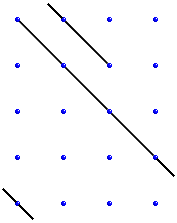
\includegraphics[width=2in]{cyclic}
\caption{A partial line through $C_{20} = C_4 \times C_5$.}
\label{cyclattice}
\end{figure}
\end{proof}
This statement is in fact equivalent to the Chinese Remainder Theorem (Theorem~\ref{crt}).
\begin{ex}
For a ``random'' Abelian group of order $n$, how often do the different types show up (e.g. $C_8$ versus $C_4\times C_2$ versus $C_2\times C_2\times C_2$)? Though this is a fuzzy question, it is possible to obtain an intuitive sense of the answer if not a concrete formula.
\end{ex}
\begin{defn}
A homomorphism from a group $G$ to a group $H$ is a function $f:G\to H$ such that $f(xy) = f(x)f(y)$.
\end{defn}
\begin{defn}
The kernel of a homomorphism $f$ is the set $\Ker f = \{x:f(x) = 1\}$.
\end{defn}
For example, on the group $\Z/p\Z \times \Z/q\Z$, then $f$ given by $x\to x^p$ has kernel $\Z/p\Z\times \{0\}$ (or the set of $(a,0)$ pairs). $f$ is only a homomorphism if the group is Abelian, since in general $(xy)^p = x^p y^p$ requires commutativity.
\begin{ex}[Cayley's Theorem]
Suppose $G$ is a finite Abelian group with order $k$ that divides some prime $p$. Show that some element of the group has order $p$ (i.e. that there is a cyclic subgroup with order $p$).

Hint: It will be helpful to consider $p$ elements of the group such that $\prod_{i=1}^p x_i = 1$ (e.g. $x_i= 1$ or $x, x^{-1}, 1, 1,\dots$, etc.). In particular, $y\cdot y\dotsb y =1$ if $y$ has order $p$. Then, count them in a way that considers order (relative, given by $a$ after $b$, or absolute, for permutations).
\end{ex}
%\begin{proof}[Solution]
%$G$ can be written as $G = C_{p^k} \times G'$, where $G'$ is some other Abelian group, and there exists an element of order $p$ in $G$ if there's one in $C_{p^k}$, since that element $a\in C_{p^k} \to (a,1)\in G$.

%Since $C_{p^k} \cong \Z/p^k\Z$, then the element corresponding to $p^{k-1}$ has order $p$ in $C_{p^k}$ and thus $G$.
%\end{proof}
\begin{cor}
The 2-torsion subgroup of a finite Abelian group (i.e. those elements that square to the identity) has size $2^k$ for some $k$.
\end{cor}%Which implies things about genera!
This implies things about the genera of reduced quadratic forms.
\begin{defn}
The principal genus is the genus of reduced quadratic forms that contains the identity element of the class group (i.e. either $x^2+ny^2$ or $x^2+xy+ny^2$).
\end{defn}
The principal genus is a subgroup of the class group $G$ given by $G^2 = \{x^2: x\in G\}$ and the remaining genera are its cosets. Thus, the number of genera is $|G|/|G^2|$.
\begin{claim}
The number of genera of a given class group is the number of 2-torsion elements it contains (including the identity).
\end{claim}
\begin{proof}
Consider the homomorphism $\varphi: G \to G^2$. Then, the 2-torsion subgroup $A_{T_2}$ of $G$ is just $\Ker(\varphi)$.

Since $\varphi$ is surjective, then by the First Isomorphism Theorem (Exercise~\ref{firstiso}), $G / \Ker(\varphi) \cong G^2$. This means that $|G|/|G^2| = |A_{T_2}|$.
\end{proof}
From this, one can easily compute the size of each genus: since they are cosets of the principal genus $G^2$, then they all have the same size, which is $|G|/|A_{T_2}| = |G^2|$.

This can be reformulated in terms of the ideal class groups, where the identity is $(1)$ and the inverse of $(a,b)$ is $(a,-b)$ (and $(a)^{-1} = (a)$). In this case, the principal genus is the set of squares of ideals (or for each ideal, the smallest ideal containing all the products of elements in that ideal).

    \section{Some Background on Groups: July 24, 2012}
	\subsection{Some Preliminaries}
\begin{defn}
A group is a set $G$ with an identity element $e\in G$ and an operation $\cdot: G\times G\to G$ such that:
\begin{enumerate}
\item $\cdot$ is associative,
\item $e\cdot g = g\cdot e = g$ for all $g\in G$, and
\item $\forall g\in G$ $\exists g^{-1}\in G$ such that $gg^{-1} = g^{-1}g = e$.
\end{enumerate}
\end{defn}
\begin{defn}
The order of a group, denoted $\ord G$ or $\card G$, is the number of elements it contains, or is infinite if the group contains infinitely many elements.
\end{defn}
\begin{defn}
A subgroup of a group $G$ is a subset $H$ of $G$ that forms a group under the same operation. Subgroups are denoted $H\le G$.
\end{defn}
\begin{defn}
A (left) coset of a subgroup $H\subseteq G$ is a set $gH = \{gh: h\in H\}$.
\end{defn}
\begin{defn}
If $H\subseteq G$ is a subgroup, then the quotient $G/H$ (read $G$ mod $H$) is the set of left cosets of $H$.
\end{defn}
Inside of the Klein-four group $G = \Z/2\Z \times \Z/2\Z$, the set $H = \{(0,0),(1,0)\}$ is a subgroup whose cosets are $H$ and $G\setminus H$.
\begin{lem}
The sizes of the cosets for a subgroup are the same: $|gH| = |g'H|$.
\end{lem}
\begin{proof}
The bijection $g'g^{-1}$ sends $gH$ to $g'H$ (by group property, it is invertible), so the cosets have the same size.
\end{proof}
\begin{lem}
Any 2 cosets of $H$ are equal or disjoint.
\end{lem}
\begin{proof}
Suppose $gH$ and $g'H$ have some element in common, so $\exists x\in gH\cap g'H$. Then, since $x = gh = g'h'$ for some $h,h'\in H$, then $g = g'h'h^{-1}$. But since $H$ is a group, then $h'h^{-1} H = H$, so $gH = g'(h'h^{-1} H) = g'H$.
\end{proof}
\begin{thm}
Let $H$ be a subgroup of a finite group $G$. Then, $\card H$ divides $\card G$.
\end{thm}
\begin{proof}
Since all left cosets of $H$ have the same size and are disjoint, and every element of $G$ belongs to some coset of $H$, then\footnote{$\bigsqcup$ is used to denote the disjoint union of sets.}
\[G = \bigsqcup_i g_iH \quad \implies \card G = \card{G/H}\cdot \card H.\qedhere\]
\end{proof}
\begin{cor}[Lagrange]
The order of any $g\in G$ divides $\ord G$.
\end{cor}
\begin{proof}
Since every element generates a subgroup of its order, then that order must divide $\ord G$.
\end{proof}
\begin{defn}
A group action of a group $G$ on a set $X$ is a map $\cdot: G\times X\to X$ such that if $g,g'\in G$ and $x\in X$, then $(gg')\cdot x = g\cdot (g'\cdot x)$ and $1\cdot x = x$.
\end{defn}
\begin{ex}
Verify that $G$ always acts on $G/H$ on the left by the map $g\cdot aH = gaH$.
\end{ex}
\begin{proof}[Solution]
Suppose $g,g',a\in G$, so that $aH \in G/H$. Then, $(gg')\cdot aH = (gg'a)H$ and $g\cdot(g'\cdot aH) = g\cdot(g'aH) = (gg'aH)$, and $1\cdot aH - (1a)H = aH$. Thus $\cdot$ is a group action.
\end{proof}
\begin{defn}
A subgroup $H\subseteq G$ is normal, denoted $H \!\vartriangleleft G$, if $gH = Hg$, or equivalently, $gHg^{-1} = H$ for all $g\in G$.
\end{defn}
\begin{ex}
Show that if $H\!\vartriangleleft G$, then $G/H$ has a group structure given by $gH \cdot g'H = gg'H$.
\end{ex}
\begin{proof}[Solution]
Suppose $g'H$ is an inverse of $gH$ in $G/H$. Then, $gH\cdot g'H = H$, so $gH\cdot g'Hg = Hg = gH$, so left-multiplying by $g^{-1}H$, $g'Hg = H$, so $g' = g^{-1}$. Thus, the inverse is unique.

The other group properties are trivial, since each can be taken from $G/H$ to $G$, where they already hold.
\end{proof}
Thus, one way to think of a group structure is a group acting upon itself: $G\times (G/H) \to G/H$. If $H\!\vartriangleleft G$, then $H \times (G/H) \to G/H$ acts trivially (i.e. it is the projection to right coordinates, so the element of $H$ is ignored. Thus $H$ is the kernel of this action).
\begin{defn}
An automorphism of a set $X$ is a bijection from $X$ to itself. The set of automorphisms of a given $X$ is denoted $\Aut(X)$.
\end{defn}
\begin{ex}
Show that a group action of a group $G$ on a set $X$ is the same as a map $f:G\to\Aut (X)$.
\end{ex}
\begin{proof}[Solution]
For any $g\in G$, a group action $f:G\times X \to X$ defines a map $h: x\mapsto f(g,x)$. The map $h^{-1}(x) = f(g^{-1},x)$ satisfies
\[h(h^{-1}(x)) = h^{-1}(h(x)) = f(gg^{-1},x) = f(1,x) = 1,\]
so $h: X\to X$ is a bijection. Thus $f:G\to\Aut(X)$.
\end{proof}
In some cases this is a group homomorphism (since group homomorphisms preserve group actions).

Given this, $H\subset\Ker f$, so $f(H) = e$ (the identity).
\begin{defn}
The image of a map $f$ is the set $\Im f = \{y\in H\mid\exists x\in G: y = f(x)\}$.
\end{defn}
\begin{ex}[$1^{\mathrm{st}}$ Isomorphism Theorem]
\label{firstiso}
Show that if $f:G\to H$ is a group homomorphism, then:
\begin{enumerate}
\item \label{imiso} $\Im(f) \le H$,
\item $\Ker f \!\vartriangleleft G$, and
\item \label{bij}$G/(\Ker f) \simeq \Im f$.
\end{enumerate}
In particular, verify that the bijection for item~\ref{bij} is well-defined.
\end{ex}
\begin{proof}
\begin{enumerate}
\item Since $H$ is a group, then associativity must hold in $\Im(f)$.
\begin{itemize}
\item Closure: if $a,b\in\Im(f)$, then $a = f(g),b = f(g')$ for some $g,g'\in G$, so $f(gg') = f(g)f(g') = ab)$.
\item Identity: given by $f(1)$: $f(g)f(1) = f(g\cdot 1) = f(g) = f(1\cdot g) = f(1)f(g)$.
\item Inverses: if $a=f(g)$, let $a'=f(g^{-1})$, so $aa' = f(g)f(g^{-1}) = f(gg^{-1}) = 1$ and similarly with $a^{-1}a$.
\end{itemize}
Thus, $\Im f\le H$.
\item By the proof of~\ref{imiso}, the identity satsifies $f(1) = 1$, so $1\in\Ker f$. Associativity in $\Ker f$ also follows, since $G$ is a group.
\begin{itemize}
\item Closure: if $g,g'\in\Ker f$, then $f(gg') = f(g)f(g') = (1)(1) = 1$.
\item Inverses: if $g\in\Ker f$, then $g^{-1}\notin \Ker f$ implies $f(g)f(g^{-1})\ne 1$, but $f(gg^{-1})$.
\item Normality: if $g\in G$, then $gH = \{a\in G: f(a)=f(g)\}$ ($\subset$ is by definition; $\supset$ is because $f(a) = f(g)\implies f(a)\cdot 1 = f(g)$, so $ah = g$ for some $h\in H$).

Similarly, $Hg = \{a\in G:f(a) = f(g)\}$ by a similar line of reasoning; $\subset$ follows by definition, and $\supset$ is true because $f(a) = f(g)\implies 1\cdot f(a) =f(g)$, so for some $h\in H$, $ha = g$.
\end{itemize}
Thus, $\Ker f \!\vartriangleleft G$.
\item Define a map $h: G/(\Ker f) \to \Im f$ given by $h(A) = f(g)$ for $g\in A\in(G/\Ker f)$. This is well-defined because all $g\in A$ have the same value $f(g)$ (since $a = b\Ker f$ for some $b\in G$ implies $f(g) = f(b)$ for all $g\in A$).

The inverse is also well-defined: for any $x\in \Im f$, there exists a $g\in G$ such that $f(g) = x$, so $g(\Ker f)$ is a coset in $G/(\Ker f)$. If $x,x'$ are distinct in $\Im f$, then they must have distinct preimages, since all elements in a coset have the same value.

The group structure is preserved because $f$ is a homomorphism and $h$ is well-defined, so $h$ is one as well.

Thus, $G/(\Ker f) \simeq \Im f$.
\end{enumerate}
\end{proof}
\subsection{Some Examples of Groups}
Groups often arise due to symmetries in some object. For example, the group of automorphisms of a tetrahedron is $S_4 = \Aut(\{1,2,3,4\})$ (which can be seen by numbering the corners of the tetrahedron $1,\dots,4$; the group $S_4$ is just the set of permutations of 4 elements). This does not work as nicely for all the Platonic solids -- the icosahedron's symmetry group has order 60, and is unpleasant to work with.

Interestingly, the Klein-four group $A_4$ satisfies $A_4\!\vartriangleleft S_4$.

The set of $2\times 2$ matrices with nonzero determinant (which is necessary for invertibility) and complex entries forms a group called $\GL{2}(\C)$. Notice that $\det\!: \GL{2}(\C) \to \C^\times$ is a group homomorphism and $\Ker(\det) = \SL{2}(\C)$. The upper triangular matrices in this group are an abnormal subgroup of $\GL{2}(\C)$. One can also define the unitary matrices (those with determinant 1) $\mathrm{U}(2)$.

There are also some interesting Abelian groups, such as $\Q$ or $\R$ under addition, $\Z$, number fields, or any ring. One also has the $p$-adic units (i.e. the $p$-adic numbers with nonzero first digit).

The circle group is the set of points on the unit circle, with group operation defined by adding arguments. This can be constructed as $\{x\in\C: |x| =1\}$ or $\R/\Z$ or $\SL{1}(\C)$.

Another example is the group of diagonal matrices with nonzero entries, given by $\C^\times \times \dots\times \C^\times$. All of these groups represent symmetries of some sort.
\subsection{More Group Actions and Abelian Groups}
Every normal subgroup $H$ is the kernel of some group action, because there exists some $f:G \to G/H$, which is a homomorphism.

A group can act on itself in a trivial manner, through $G\to\Aut(G)$, but there is another path by group homomorphism. This can still be trivial, but it can also create a $g\cdot x\in G$ given by $gxg^{-1}$ (since it is necessary for $1\to 1$.)
%\subsection{Abelian Groups}
%\label{struct}
\begin{defn}
An abelian group is a group for which the operation is commutative (i.e. $ab = ba$ for all $a,b\in G$).
\end{defn}
Every subgroup of an Abelian group is therefore normal.

These include the cyclic groups and their products, but also $\Z$ (sometimes called the infinite cyclic group) and $\Q$, $\R$, and $\C$.

\begin{ex}
If $A$ is a finitely generated abelian group and $B < A$, show that $B$ is finitely generated.
\end{ex}
%\begin{thm}
%Any finitely generated abelian group is of the form
%$\Z^k \times \prod_{i=1}^r \Z/n_i\Z$ for some $k,r,n_i\in N$.
%\label{fgag}
%\end{thm}
%\begin{lem}
%Let $A$ be a torsion-free abelian group.\footnote{i.e. all of the elements of $A$ have infinite order. This implies $A$ has infinite order as well, but the converse is not true, as in $\prod_{i=1}^{\infty} \Z/2\Z$.} Then, $A\simeq \Z^k$ for some $k\in\N$.
%\label{torsionlemma}
%\end{lem}
%\begin{proof}
%Pick a minimal set of generators (i.e. the set of generators of the smallest size) $x_1,\dots,x_n\in A$ (see Exercise~\ref{genset}). Then, every $a\in A$ can be written as $a = \sum_{i=1}^n a_ix_i$, where $a_i\in\Z$. Thus, there is an isomorphism between $A$ and $\Z^n$ given by setting $x_i\simeq \vec e_i$ and $0 \simeq (0,\dots,0)$, since the generators are linearly independent (since they are a minimal set).
%\end{proof}
%\begin{ex}
%\label{genset}
%Show that a torsion-free abelian group can be generated by some finite set. Hint: use induction.
%\end{ex}
%\begin{ex}
%\label{secondlemma}
%Suppose $A,B$, and $C$ are abelian groups and $A\to B\stackrel{g}{\to} C$ is a sequence of maps such that $A\hookrightarrow B = \Ker g$. Then, if there exists some $q:C\to B$ such that $g\circ q = e$ (i.e. the identity) on $C$, then $B\simeq A\oplus C$.%Assume this is a homomorphism?
%\end{ex}
%\begin{proof}[Proof of Theorem~\ref{fgag}]
%The case of torsion-free abelian groups is taken care of by \hyperref[torsionlemma]{the lemma}, so suppose $A$ is an abelian group with torsion. Take the torsion subgroup $T\!\vartriangleleft A$, defined as all elements which are torsion (i.e. of finite order). Then, one can define maps $T \stackrel{g}{\hookrightarrow} A \stackrel{f}{\twoheadrightarrow} A/T$, where $g$ is the injection given by inclusion and $f$ is the canonical surjection $A\twoheadrightarrow A/T$ given by placing each element in its coset. Thus, $\Ker f = T$, so $f\circ g = e$.
%
%The map $g\oplus f^{-1}:T\oplus \Z^k \to A$ can be made by sending each basis element to any of its preimages. Thus, there exists a map $\pi:(x,y)\mapsto g(x) + f(y)$, where $x\in T$ and $y\in\Z^k$. Then, $\Ker \pi = T$.
%
%$\pi$ is surjective: given some $a\in A$, then $f(\pi(a))\in A$ and $\pi(a-f(\pi(a))) = 0$ (because $f(x)$ will be torsion-free). Thus, $a - f(\pi(a))\in T$, so $a = f(\pi(a)) + t$ for some $t\in T$.
%\begin{ex}
%Check that $\pi$ is an injection and a group homomorphism.
%\end{ex}
%Given this property of $\pi$ and using Exercise~\ref{secondlemma}, $A \simeq T\oplus \Z^k$.
%
%Now consider a finite abelian group $A$; let $N$ be the largest order of any element in $A$, and let $A'$ be the group generated by all elements of order $N$. Thus, one has maps $A'\hookrightarrow A \twoheadrightarrow A/A'$. By induction on $N$ and strong induction on $|A|$, $A/A' = \prod \Z/n_i\Z$ for $n_i < N$.
%
%Let $B$ be a group generated by one element of order $N$. Then, one can define the sequence of maps
%\[B \simeq \Z/N\Z \stackrel{g}{\to} A\stackrel[\pi]{f}{\leftrightarrows}\prod_i \Z/n_i\Z \simeq A/A'\] in the same manner as above. In particular, $g\in\Ker\pi$, so using the same line of thought as above, $\pi f = 1$. Thus, using Exercise~\ref{secondlemma}, $A$ is the product of cyclic groups $\Z/n_i\Z$.
%\end{proof}

    \section{Computations in Quadratic Fields: July 26, 2012}
	Recall that the ring of integers $\cO_K$ has unique factorization of ideals (which is rather difficult to prove).
\begin{thm}[Chinese Remainder Theorem]
\label{crt}
Given some distinct primes $p_i$, then the system $x \equiv a_i\mod p_i$ has a unique solution $\mod \prod_i p_i$.
\end{thm}
(This also works if $p_i$ are any relatively prime numbers.)

For example, if $x\equiv 4\mod 5$, $x\equiv 0\mod 2$, and $x \equiv 0\mod 3$, then $x\equiv 24\mod 30$.

There are several alternate formulations to the Chinese Remainder Theorem:
\begin{thm}
Suppose $n$ has the prime factorization $n = \prod_{i=1}^r p_i^{e_i}$. Then,
\[\Z/n\Z \simeq \prod_{i=1}^r \Z/p_i^{e_i}\Z.\]
\end{thm}
As in the previous example, $\Z/30\Z = \Z/2\Z\times\Z/3\Z\times \Z/5\Z$, and $24\to (0,0,4)$.
\begin{thm}[Chinese Remainder Theorem for Ideals]
\label{crtideals}
Let $\fp_i$ be distinct prime ideals of some ring of integers $\cO_K$. Then,
\[\cO_K / \prod_i \fp_i^{e_i} \simeq \prod_i \cO_K/\fp_i^{e_i}.\]
\end{thm}
Consider the Gaussian integers $\Z[i]\subset\Q(i)$.\footnote{The notational difference between $\Q[i]$ and $\Q(i)$ is subtle. The former allows addition, subtraction, and multiplication (i.e. constructs a ring), but the latter also allows for division (making it a field). However, since $\Q$ is already a field, $\Q[\sqrt{-D}] = \Q(\sqrt{-D})$, and in these cases it does not matter.}

They can also be thought of as $\Z[x]/(x^2+1)$, which is isomorphic to $\Z[i]$. Notationally, $K[x]$ is the ring of polynomials over the ring $K$, and $(x^2+1)$ is the set $\{(x^2+1)p(x):p(x)\in\Z[x]\}$. This is because $x^2+1 = 0$ is equivalent to $x^2\equiv -1$ when modding out by $x^2+1$. In particular, since $x^2\equiv -1$, then
\[(a+bx)(c+dx) = ac+(ad+bc)x+bdx^2 = (ac-bd) + (ad+bc)x \simeq (a+bi)(c+di).\]
Some interesting things can be passed into the Chinese Remainder Theorem:
\[\Z[i][x]/(x^2+1) \simeq \Z[i][x]/(x+i) \times \Z[i][x]/(x-i).\]
The ideals $(x+i)$ and $(x-i)$ are both prime because of degree.

It will be helpful to have a more intuitive understanding of the multiplication of ideals: consider $(2,1+\sqrt{-5}),(2,1-\sqrt{-5})\in\Z[\sqrt{-5}]$. Multiplication of ideals involves multiplying the elements together, but also eliminating dependencies:
\[(2,1+\sqrt{-5})(2,1-\sqrt{-5}) = (4,2-2\sqrt{-5},2+2\sqrt{-5},6) = (2)\] because $2(2) = 4$, $2(3) = 6$, and $2(1\pm \sqrt{-5}) = 2\pm 2\sqrt{-5}$.

Consider the quotient $\Z[i]/(5) = \Z[i]/(2+i) \times \Z[i]/(2-i)$. In this ring, $\alpha = \beta$ iff $\alpha \equiv \beta \mod (5)$ in $\Z[i]$. Thus, it can be thought of as a $5\times 5$ lattice in which the ends are identified, as on a torus.
\begin{defn}
The norm of an ideal $I$ is $|\cO_K/I|$.
\end{defn}
In particular, $N((5)) = 25$, given the $5\times 5$ lattice seen above. In general $N((k)) = N(k)$ (norm of an ideal vs. norm of a number); the proof relies on a geometry-of-numbers argument very similar to the one presented in Section~\ref{geoofnum} and considers $\cO_K$ as a lattice.

It is also true that $N(\alpha\beta) = N(\alpha)N(\beta)$, as with the norm on $\C$; the proof follows from the above for the case of single-generated ideals and is a little more complicated otherwise.\footnote{This property of the norm holds in number fields, but not everywhere: $|\R[x]/(x^2+1)| =\infty.$} Thus, if $I,J$ are relatively prime ideals, then $\cO_K/(IJ) = \cO_K / I \times \cO_K/J$.

This can be used to check whether an ideal is prime: since $(5) = (1+2i)(1-2i)$ in $\Z[i]$, then $N(1+2i) = N(1-2i) = 5$ (since $N((5)) = 25$). Since 5 is prime over $\Z$, then $(1\pm 2i)$ are both prime. The converse, however, is not true: $N((3)) = 9$, but if $3 = \fp_1\fp_2$, then $N\fp_1 = 3$, so $9 = (a^2+b^2)(c^2+d^2)$ where $a^2+b^2 = 3$ over $\Z$, which doesn't work.

Consider the following equivalent rings:
\[\Z[i]/(5) \simeq \Z[x]/(x^2+1,5) \simeq(\Z[x]/(x^2+1))/(5)\simeq \mathbb F_5[x]/(x^2+1).\]
It happens that the First Isomorphism Theorem (see Exercise~\ref{firstiso}) also holds for rings; both the statement and the proof are identical. Thus, consider the map $\Z[x] \stackrel{f}{\to} \mathbb F_5[x]/(x^2+1)$ such that $1\to 1$, $x\to x$, and $f(a+b) = f(a)+f(b)$. This implies that $\Ker f = (5,x^2+1)$.

Notice that $x^2+1 \equiv (x+2)(x+3)\mod 5$, and that $x^2+2$ is irreducible. However, one can show that if $K$ is a field, then $K[x]$ is a PID, and since $\mathbb F_5$ is a field, then there is unique factorization about irreducibles. Additionally, by the Chinese Remainder Theorem (specifically, formulation~\ref{crtideals}), if $f$ is irreducible, then $(f)$ is prime.
\begin{claim}
This gives rise to some more isomorphisms:
\[\Z[i]/(5)\simeq \mathbb F_5[x]/(x+2)\times \mathbb F_5[x]/(x+3) \simeq \mathbb F_5\times \mathbb F_5.\]
\end{claim}
\begin{proof}
Consider the map $\mathbb F_5[x] \stackrel{g}{\to} \mathbb F_5$ such that $g(1) = 1$, $g(x) = 2$ (or 3), and $\Ker g = (x+2)$ (or 3). For the last map, just subtract 2 or 3 from each element.
\end{proof}
Similarly, because 3 is prime in $\Z[i]$, $\Z[i]/(3) \simeq \mathbb F_3[x]/(x^2+1)$ is also prime.

In general, one can determine the decomposition of a prime $p$ by factoring $(x^2+1)$ into two quotients. There are three possibilities:
\begin{enumerate}
\item $(p)$ is prime in $\Z[i]$ iff $(x^2+1)$ is irreducible in $\mathbb F_p[x]$, in which case $p$ is called inert. This requires $x^2+1\not\equiv 0$, so happens iff $p \equiv 3\mod 4$.
\item If $(x^2+1) = (x+a)(x+b)$ for distinct $a,b$, then $p$ splits in $\Z[i]$, which happens iff $p \equiv 1\mod 4$ (because that is the requirement for $-1$ to be a quadratic residue).
\item If $(x^2+1) = (x+a)^2$, then $p$ is ramified. 2 is the only ramified prime (and $a = 1$).
\end{enumerate}
Recall that the class group was defined as ideals up to the equivalence relation $\mathfrak a \sim \mathfrak b$ iff $c\mathfrak a = d\mathfrak b$ for $c,d\in\cO_K$.\footnote{When handwritten, it is common to use $\underline{a},\underline{b},\underline{\smash p}$ instead of $\mathfrak a,\mathfrak b,\mathfrak p$.} For example, in $\Z[i]$, $(2)\sim (4)$ and $(2)\sim (2,2+2i)\sim (1)$. In $\Z[\sqrt{-5}]$, $(2,1+\sqrt{-5}) \nsim (1)$.
\begin{thm}
Suppose that $K = \Q(\sqrt{-D})$ and $D_K$ is its discriminant as defined in Section~\ref{qfields}. If $C$ is an ideal class, then there exists an ideal $I\in C$ such that $N(I) \le \frac{2}{\pi}\sqrt{|D_K|}$.
\end{thm}
This proof also relies on a geometry-of-numbers argument like the Four-Squares Theorem (Theorem~\ref{foursquare}). The idea is that $\cO_K$ is the set of intersections of some lines, and that $I$ is a sublattice. Then, $|I|$ is the area of the fundamental \pgram{} relative to $\cO_K$. Then, by Minkowski's Theorem (Theorem~\ref{mink}), there has to be a nontrivial lattice point eventually.

For example, all ideals in $\Z[i]$ must contain an ideal of norm $N<2$ ---  but if $N\in\N$, then there is only one equivalence class, so the class group is the trivial group $C_1$.

As another example, consider $\Q[\sqrt{-5}]$, for which $D_K = -20$, so every ideal class contains an ideal of norm $\le \frac{2}{\pi}\sqrt{20} < 3$. The trivial ideal (i.e. $(1)$) has order 1, but $(2)$ factors as
\[\Z[-5]/(2) \cong (\Z[x]/(x^2+5))/(2) \cong\mathbb F_2[x]/(x^2+5).\]
This does factor, since $(x+1)^2 \equiv x^2+5\mod 2$, so $(2) = \fp^2$ is ramified. Since $N(2) = 4$, then $N(\fp) = 2$, so there must be some other ideal with norm 2. $\fp = (x+iy)$ is not principal, but $\fp^2 = (2)$ is.
Thus there are two distinct classes of ideals and $h(-20) = 2$.
\begin{ex}
Using this method, calculate the class group of $\Q[\sqrt{-26}]$.
\end{ex}
These techniques can also be used to answer the questions raised in Section~\ref{use}. The older ($18^{\mathrm{th}}$--\,Century) formulation of a question might be that $x^2+5y^2 = p$ iff $p \equiv 1,9\mod 20$ and $x^2+2xy+3y^2 = p$ iff $p \equiv 3,6\mod 20$, and otherwise, $\jac{-20}{p} = -1$, so there is no such representation.

However, with quadratic fields, writing a prime of the form $p = x^2+5y^2$ is akin to aking if there is a principal ideal of norm $p$ in $\Z[\sqrt{-5}]$. If $(p)$ splits or is ramified (which in this case could be both 2 and 5), then there is such an ideal. (This statement is isomorphic to the statement that equivalent quadratic-forms represent the same integers in Section~\ref{use}).
\begin{ex}
When does $2p = x^2+5y^2$ have a solution?
\end{ex}
%\tbc

    \section{Short Exact Sequences: July 31, 2012}
	%Hopefully these results about sequences will illuminate some of the ideas in Sections~\ref{struct} and~\ref{tryagain}.
\begin{defn}
A short exact sequence is $A\stackrel{f}{\hookrightarrow} B \stackrel{g}{\twoheadrightarrow} C$ for groups $A,B,C$ such that $\Im f = \Ker g$.
\end{defn}
An exact sequence is a composition of short exact sequences (so that the image of one map is the kernel of the next). Notationally, it is common to write a short exact sequence as $0\to A\to B\to C\to0$, emphasizing its properties. (if the groups are written multiplicatively, $1$ is used instead of $0$.)
\begin{defn}
Given a short exact sequence of groups $0\to A\stackrel{f}{\to} B\stackrel{g}{\to} C\to 0$, a section is a group homomorphism $s:C\to B$ such that $g\circ s = \id_C$.
\end{defn}
From this definition, $s$ is injective, so $\Im s\simeq C$.

Consider the two short exact sequences
\[
\begin{tabular}{c @{$\to$} c @{$\to$} c @{$\to$} c @{$\to$} l}
$0$ & $\Z/2\Z$ & $\Z/4\Z$ & $\Z/2\Z$ & $0$\\
$0$ & $\Z/2\Z$ & $\Z/2\Z\times \Z/2\Z$ & $\Z/2\Z$ & $0$.
\end{tabular}
\]
For the second sequence, the maps $f:a\mapsto (a,0)$ and $g:(a,b)\mapsto b$ define a short exact sequence for which $s: b\mapsto(0,b)$ is a section. However, the first such sequence actually doesn't have a section: $f: a\mapsto 2a$ and $g:\Z/4\Z \to (2\Z)/(4\Z)$ define a short exact sequence, but none of the possible maps $\Z/2\Z \to \Z/4\Z$ are sections. Of course, one could define a set-theoretic section using preimages, but this is not a group homomorphism.
\begin{defn}
A short exact sequence is split if there exists a section.
\end{defn}
\begin{thm}
\label{splitting}
If $0\to A\to B\to C\to 0$ is a short exact sequence of Abelian groups with maps $f:A\to B$ and $g:B\to C$ with a section $s$, then $B \simeq A\times C$ (or, equivalently, $B\simeq A\oplus C$).
\end{thm}
\begin{proof}
Suppose $a\in A$, $b\in B$, and $c\in C$. Then,
\begin{align*}
g(b-s(g(b))) & = g(b) - g(s(g(b)))\\
&= g(b) - g(b) = 0,
\end{align*}
so $b-s(g(b))\in A$, and $b = s(g(b)) + a$ for some $a$, so $s$ is surjective. This sum is unique: if $a+s(c) = a'+s(c')$, then $g(a+s(c)) = g(a'+s(c')) = g(s(c)) = c = g(s(c')) = c'$, and since $c = c'$, then $a = a'$ as well.
\end{proof}
In this language, the fundamental theorem for finitely generated abelian groups (Theorem~\ref{fgagtheorem}) reduces to asserting that if $G$ is abelian of order $p^b$ for some prime $p$ and $x\in G$ is of maximal order, then
\[0\to\langle x\rangle \to G\to Q\to 0\]
is a short exact sequence, where $Q = G/\langle x\rangle$. The inductive assumption is that $Q$ is a product, and since $|G|/|\langle x \rangle| = |Q|$, then this can be used to justify that $G$ also is. The big question in this proof is how to show that the sequence splits.

Precautionary remark: in for non-abelian groups, splitting implies decomposition into a semidirect product, not a direct one. For example, the dihedral group of six elements\footnote{Notational conflict; some write $D_n$ for the dihedral group of $n$ elements; others use it to designate the group of symmetries of the regular $n$-gon. In this case, what I have called $D_6$ can also be written $D_3$.} $D_6$ is the set of symmetries of an equilateral triangle. It is given by the presentation $D_6 = \langle \sigma,\tau:\sigma^3 = 1,\tau^2 = 1,\tau\sigma = \sigma^3\tau\rangle$. $\sigma$ represents a rotation by $120^\circ$ and $\tau$ represents a reflection. Notice that $\langle\sigma\rangle = C_3$ and $\langle\tau\rangle = C_2$, but $D_6$ is non-abelian, so $D_6 = C_3 \rtimes C_2$, and the sequence $1\to C_3\to D_6\to C_2\to 1$ splits.

Another reason splitting can be confusing is that it doesn't extend nicely to vector spaces. Thanks to the rank-nullity theorem, a short exact sequence of vector spaces \emph{always} splits.

    \section{Finitely Generated Abelian Groups: July 31, 2012}
	%\documentclass{amsart}
%\usepackage[margin=0.75in]{geometry}
%\usepackage{microtype,hyperref,amsthm,amssymb}
%\newcommand{\Z}{\mathbb Z}
%\newcommand{\inj}{\hookrightarrow}
%\newcommand{\surj}{\twoheadrightarrow}
%\DeclareMathOperator{\Ker}{Ker}
%\DeclareMathOperator{\qwsa}{Im}
%\def\Im{\qwsa}
%\DeclareMathOperator{\id}{id}
%\renewcommand{\vec}{\mathbf}
%\newtheorem{thm}{Theorem}
%\newtheorem{lem}{Lemma}
%\theoremstyle{definition}
%\newtheorem*{defn}{Definition}
%\begin{document}
%\title{The Structure Theorem for Finitely Generated Abelian Groups}
%\author{Arun Debray}
%\maketitle
%\subsection{Short Exact Sequences} %All sections changed to subsections
%\begin{defn}
%A short exact sequence is $A\stackrel{f}{\hookrightarrow} B \stackrel{g}{\twoheadrightarrow} C$ for groups $A,B,C$ such that $\Im f = \Ker g$.
%\end{defn}
%\begin{defn}
%Given a short exact sequence of groups $0\to A\stackrel{f}{\to} B\stackrel{g}{\to} C\to 0$, a section is a group homomorphism $s:C\to B$ such that $g\circ s = \id_C$.
%\end{defn}
%From this definition, $s$ is injective, so $\Im s\simeq C$.
%\begin{defn}
%A short exact sequence is split if there exists a section.
%\end{defn}
%\begin{thm}
%\label{splitting}
%If $0\to A\to B\to C\to 0$ is a short exact sequence of abelian groups with maps $f:A\to B$ and $g:B\to C$ with a section $s$, then $B \simeq A\times C$ (or, equivalently, $B\simeq A\oplus C$).
%\end{thm}
%\begin{proof}
%Suppose $a\in A$, $b\in B$, and $c\in C$. Then,
%\begin{align*}
%g(b-s(g(b))) & = g(b) - g(s(g(b)))\\
%&= g(b) - g(b) = 0,
%\end{align*}
%so $b-s(g(b))\in A$, and $b = s(g(b)) + a$ for some $a$, so $s$ is surjective. This sum is unique: if $a+s(c) = a'+s(c')$, then $g(a+s(c)) = g(a'+s(c')) = g(s(c)) = c = g(s(c')) = c'$, and since $c = c'$, then $a = a'$ as well.
%\end{proof}
\subsection{Torsion-Free Finitely Generated Abelian Groups}
%This ends up not being necessary...
%\begin{lem}
%If $A$ is a finitely generated abelian group and $B < A$, then $B$ is finitely generated.
%\end{lem}
%So apparently I am able to assume this.
%\begin{lem}
%Any finitely generated abelian group has a minimal set of generators.
%\end{lem}
\begin{thm}[Structure Theorem for Torsion-Free Finitely Generated Abelian Groups]
\label{torsionfree}
If $A$ is a torsion-free\footnote{i.e. all of the elements of $A$ have infinite order. This implies $A$ has infinite order as well, but the converse is not true, as in $\prod_{i=1}^{\infty} \Z/2\Z$.} abelian group, then $A\simeq \Z^k$ for some natural number $k$.
\end{thm}
\begin{proof}
Let $\langle x_1,\dots,x_n\rangle$ be the minimum generating set for $A$ (such a set exists because $A$ is finitely generated). Let $f: x_j\mapsto\vec e_j\in\Z^k$ and $f(g+g') = f(g)+f(g')$. Then, $f$ is a bijection, since any element of $\Z^k$ can be sent by its basis elements via $f^{-1}:\vec e_j\mapsto x_j$. Thus $A\simeq \Z^k$.
\end{proof}
\subsection{Finite Abelian Groups}
\begin{thm}
If $A$ is a finite abelian group, then $A \simeq \prod_{i=1}^r \Z/n_i\Z$.
\label{finite}
\end{thm}
\begin{proof}
Let $N$ be the order of $A$ and pick some element $x\in A$ of order $N$. Consider the short exact sequence
\[0\to \langle x\rangle \inj A \stackrel g\surj A/\langle x \rangle \to 0.\]
Let $\pi: A/\langle x \rangle \to A$ be given by $\pi(c) = x+ c$. Thus, $g(\pi(c)) = c$ and $\pi$ maps the identity to itself, so this sequence splits by Theorem~\ref{splitting}. Thus, $A = \langle x \rangle \times A/\langle x\rangle$.

However, $\langle x \rangle \simeq \Z/N\Z$, and using induction on the order of $A$, since the order of $A/\langle x\rangle$ is less than that of $A$, then $A = \prod_{j=1}^r \Z/n_i\Z$.
\end{proof}
\subsection{The General Theorem}
\begin{thm}[Structure Theorem for Abelian Groups]
\label{fgagtheorem}
If $A$ is a finitely generated abelian group, then \[A\simeq \Z^k\times \prod_{j=1}^r \Z/n_i\Z\] for some natural numbers $k,r,n_i$.
\end{thm}
\begin{proof}
Let $T$ be the torsion subgroup of $A$ and consider the sequence
\[0\to T\stackrel f\inj A\stackrel g\surj A/T \to 0,\]
where $f$ is given by inclusion and $g$ assigns elements of $A$ to their cosets in $A/T$. Since $\Im f = \Ker g$, then this is a short exact sequence $\pi$ that splits (the proof is the same as in Theorem~\ref{finite}).
%Show that this splits

Thus, $A = T\times A/T$. However, since $A$ is finitely generated, then $T$ is finite, so $T = \prod_{j=1}^r \Z/n_i\Z$ for some $n_i$ by Theorem~\ref{finite}, and since $T$ is the torsion subgroup then $A/T$ is torsion-free, which means that $A/T \simeq \Z^k$ by Theorem~\ref{torsionfree}. Thus,
\[A = A/T\times T = \Z^k\times \prod_{i=1}^r \Z/n_i\Z.\qedhere\]
\end{proof}
%\end{document}

    \section{The Cohen-Lenstra Heuristics: August 10, 2012}
	Suppose $K$ is some imaginary quadratic field with class group $\Cl(K)$ and $\Cl_p(K)$ is the $p$-Sylow subgroup (in this case, the $p^k$-torsion of $K$). The Cohen-Lenstra Heuristcs concern the distribution of $\Cl_p(K)$; specifically, if $A$ is some finite abelian $p$-group, it considers the limit
\begin{equation}
L = \lim_{x\to\infty} \frac{\#\{\text{$K$ is a quadratic field with } \Cl_p(K) \cong A\}}{\#\{\text{$K$ is a quadratic field with } \Disc(K) < x\}}.
\label{uglylimit}
\end{equation}
Let $p$ be an odd prime (when $p = 2$, this is the different subject of genus theory).
\begin{thm}[Cohen-Lenstra Heuristic]
If $p$ is an odd prime and $A$ is a finite abelian $p$-group, then $L$ (in Equation~\ref{uglylimit}) is inversely proportional to $\#\Aut A$: Let
\[(p)_\infty = \sum_{\text{\emph{finite abelian groups }}A} \frac{1}{\#\Aut A} = \prod_{n\ge 1} \frac{1}{1-p^{-n}},\]
so that $L = \frac{1}{(p)_\infty\#\Aut A}$.
\end{thm}
There are several justifications for this seemingly counterintuitive result.

Let $I_1,\dots,I_n$ be a lot of nonzero ideals of $K$.\footnote{To be precise, they are ideals of $\cO_K$, but this abbreviation is commonly used.} They satisfy certain relations of the form $\prod_{j=1}^n I_j^{a_j} = (b)$ (some principal ideal), so $\sum_{j=1}^n a_jI_j = \cO_{\Cl(K)}$ written additively.
\begin{defn}
If $f:G\to H$ is a homomorphism between abelian groups, then the cokernel of $f$ is $\coker f = H/\Im f$.
\end{defn}
If these $a_i$ are chosen randomly and written (over several iterations) in a matrix, then for very large $n$, the cokernel of the matrix is finite.

However, it's not actually possible to pick random integers, so instead random $p$-adic numbers have to be chosen. There are two primary ways to envision the $p$-adic numbers: they can be thought of as a collection of clopen sets as in Section~\ref{skolem}, but also as infinite strings of base-$p$ digits, trailing off to the left. Thus, starting from the units place, one can randomly pick a digit in each place, to generate a random element of $\Z_p$.
\begin{thm}[Friedman-Washington]
\label{randommatrices}
The distribution of cokernels of these random matrices in $\Z_p$ is identical to the Cohen-Lenstra distribution on class groups.
\end{thm}
\begin{thm}[Maples]
A generalization of Theorem~\ref{randommatrices} that claims the distribution does not even have to be random, thugh it must be independent.
\end{thm}
(Though it is more general, this theorem is not terribly useful.)

Another approach to this heuristic is to fix some prime power $p^r$ and randomly generate an abelian group according to the following algorithm:
\begin{enumerate}
\item Randomly generate a multiplication table, and
\item Throw it away if it's not an abelian group.
\end{enumerate}
Obviously this is horribly inefficient and isn't actually implemented on a computer, but has mathmatical significance. To be precise, the probability that a group $B$ randomly generated in this manner is isomorphic to a given $A$ is inversely proportional to $\#\Aut A$.

The automorphism group is sometimes difficult to envision, so here are some examples:

If $A = \Z/n\Z$, then $A$ is generated by a single element, so an automorphism just sends one generator to another, so $\Aut A = (\Z/n\Z)^\times$ and $\#\Aut A = \varphi(n)$.

If $A = (\Z/n\Z)^r$, then choose a basis and send each basis element to something of order $n$: $(a_1,\dots,a_r)$ with $\gcd(a_1,\dots,a_r) = 1$ (which is also equal to the least common multiple of their orders). Consider $n$ of these as column vectors and write them as a matrix $M$. In order to be an automorphism, this matrix must be invertible, so $M\in\GL{r}(\Z/n\Z)$, and thus $\Aut A = \GL{r}(\Z/n\Z)$.

The size of this automorphism group is more complicated, but when $n = p^k$ is a prime power, then $\#\Aut A = \prod_{j=0}^{r-1} \left((p^k)^r - (p^k)^{r-j}\right)$.

For example, $\Aut(\Z/9\Z) = (\Z/9\Z)^\times$, which has size 6, but $\Aut((\Z/3\Z)^2) = \GL{2}\mathbb F_3$, which has size 48. Thus, the heuristic predicts that $\Z/9\Z$ should be about eight times as common as $\Z/3\Z\times\Z/3\Z$ as a class group; however, for small discriminants, this ratio can be overshot.

    \section{The Analytic Class Number Formula: August 16, 2012}
	Suppose $p = 7$. Then, the squares $\mod 7$ are
\begin{tabular}{c c c|c c c}
$1$&$2$&$3$&$4$&$5$&$6$\\
$+$&$+$&$-$&$+$&$-$&$-$.
\end{tabular}\\
For $p = 23$ it's a bit harder, though still computable without paper:

\begin{tabular}{c c c c c c c c c c c|c c c c c c c c c c c}
$1$&$2$&$3$&$4$&$5$&$6$&$7$&$8$&$9$&$10$&$11$&$12$&$13$&$14$&$15$&$16$&$17$&$18$&$19$&$20$&$21$&$22$\\
$+$&$+$&$+$&$+$&$-$&$+$&$-$&$+$&$+$&$-$&$-$&
$+$&$+$&$-$&$-$&$+$&$-$&$+$&$-$&$-$&$-$&$-$
\end{tabular}\\
And just for one more example, here are the residues $\mod 31$:

\begin{center}
\begin{tabular}
{c c c c c c c c c c c c c c c}
$1$&$2$&$3$&$4$&$5$&$6$&$7$&$8$&$9$&$10$&$11$&$12$&$13$&$14$&$15$\\
$+$&$+$&$-$&$+$&$+$&$-$&$+$&$+$&$+$&$+$&$-$&$-$&$-$&$+$&$-$\\
\hline
$16$&$17$&$18$&$19$&$20$&$21$&$22$&$23$&$24$&$25$&$26$&$27$&$28$&$29$&$30$\\
$+$&$-$&$+$&$+$&$+$&$-$&$-$&$-$&$-$&$-$&$-$&$-$&$+$&$-$&$-$
\end{tabular}\\
\end{center}

Notice that there are more minus signs on the right-hand side of each table than on the left.

Suppose $\chi(n) = \jac{n}{p}$. Then, $\sum_{n=1}^{p-1}\chi(n) = 0$. However, since the residues are distributed unevenly, one obtains
\[
\sum_{n=1}^{\frac{p-1}{2}} \chi(n) =\left\{
\begin{array}{c l r @{\,=\,} l}
1 & p=7 & h(-7)&1\\
3 & p=23 & h(-23)&3\\
3 & p = 31& h(-31)&3.
\end{array}\right.
\]
Well, this looks suspicious. And this suspicion can be confirmed:
\begin{thm}
\label{halfsum}
If $p\equiv 3\mod 8$, then $h(p) = \displaystyle{\sum_{n=1}^{\frac{p-1}{2}}} \chi(n)$.
\end{thm}
In general, the formula is $\sum_{(x,D) = 1}^{D/2}\chi_D(x) = (2-\chi(D))h(-D)$, where $\chi_D(x) = \jac xD$ is called the quadratic character of $D$. Notice that since $\chi(D) = \pm 1$, the conjectured formula is only off by a factor of at most 3.

Now consider
\[
\sum_{n=1}^{p-1}\chi(n)n =\left\{
\begin{array}{r l}
-7 & p = 7\\-69 & p = 23\\ -93 & p = 31\end{array}\right.
\]
Once again, this looks like $\sum_{n=1}^{p-1} \chi(n)n = ph(-p)$. However, if you take only the first half, it evaluates to $\sum_{n=1}^{\frac{p-1}{2}} \chi(n)n = 0$.
\begin{thm}
\label{wholesum}
The more general version of the formula is
\[\frac{1}{|D|}\sum_{(x,D) = 1}^{D-1}\chi(x)x = h(-|D|).\]
\end{thm}
Theorems~\ref{halfsum} and \ref{wholesum} are consequences of a more general class number formula.\footnote{Much of this is going to look like magic and won't be very enlightening without some more background.}
\begin{defn}
Let $K =\Q[\sqrt D]$, $\cO_K$ be its ring of integers, and $D$ be its discriminant. Then, the zeta function $\zeta_{_K}:\C\to\C$ associated with $K$ is 
\[\zeta_{_K}(s) = \sum_{I\subset\cO_K}\Norm(I)^{-s}.\]
\end{defn}
This is where complex analysis enters into number theory. Additionally, the Riemann zeta function is just the function for $K = \Q$: $\zeta_\Z(s) = \sum_{n\in\N} n^{-s}$.
\begin{thm}
\[\lim_{s\to 1} (s-1)\zeta_{_K}(s) = \frac{2\pi}{|\cO_K^\times|}\sqrt{|D|}h(-|D|).\]
\end{thm}
In all but a few small cases, $|\cO_K^\times| = 2$, making this computation relatively straightforward. Interestingly, this theorem was first proven by Dirichlet with quadratic forms, and the modern number-field version came later.
\begin{defn}
The L-function associated with a number field is $L(s,K) = \sum_{n=1}^\infty \chi(n)n^{-s}$, where $\chi$ is the character associated with $K$ (in this case, the Legendre symbol).
\end{defn}
This gives $\zeta_{_K}(s) = \zeta(s)L(s,K)$. Since $\lim_{s\to 1} \zeta(s) = 1$, then the L-function can be used for a class number formula (which is not a closed form, since there is an infinite series involved):
\[L(1,\chi) = \frac{2\pi h(-|D|)}{|\cO_K^\times|\sqrt D}.\]
This is the source of the above formulae.

In the end, there is a class number formula, and Exercise~\ref{formula} has a solution --- albeit not one that can be easily found. It is surprisingly analytic, but also explains a couple observations:
\begin{enumerate}
\item Why the growth rate of the class number formula has to do with the Riemann Hyporthesis, and
\item Since the class number is positive, then there are more quadratic residues in the first half of $\Z/p\Z$ than in the second half. In fact, this \emph{is} the proof; no simpler one has been found.
\end{enumerate}

\chapter{Mathematical Lectures}
    \section{Factoring, by Dr. Akshay Venkatesh: June 27, 2012}
	%\documentclass{amsart}
%\usepackage{geometry,microtype}
%\geometry{margin=0.5in}
%\theoremstyle{definition}
%\newtheorem*{thm}{Theorem}
%\begin{document}
%\title{Factoring}
%\author{Dr. Akshay Venkatesh\\June 27, 2012}
%\maketitle
Given some integer $N$, what is an algorithm to generate $p,q\in\mathbb{Z}$ siuch that $N = pq$?

The first such algorithm is to divide $N$ by primes $2,3,5,\dots$ up to $\sqrt{N}$. Then, if $H$ has a factor, then one of $p,q \le \sqrt{N}$. This is inefficient, but any better method takes a bit of cleverness.

The next two methods are $O(N^{\frac{1}{4}})$, which is pretty nice. (It's actually quite easy to tell whether a number is prime, but factoring it is harder.)

The second method is a refinement of the first: you don't have to divide by every prime, because knowing information about $N/i$ allows you to know information about $N/(i+j)$ for small integers $j$.

Suppose $i \approx \sqrt{N}$, which is a reasonable assumption because this is where the first algorithm tends to spend the most time. Then, one can expand the Taylor series to conclude that
\[\frac{N}{i+1} = \frac{N}{i(1+\frac{1}{i})} = \frac{N}{i}\left(1-\frac{1}{i} +\frac{1}{i^2}-\dots\right) \approx \frac{N}{i} -\frac{N}{i^2}\]
Similarly, $\frac{N}{i+2} \approx \frac{N}{i} -\frac{2N}{i^2}$.

For example, consider $N = 295313885939$. It has a factor near $10^6$, so consider a small $j\in\mathbb{Z}$ such that $\frac{N}{10^6 + j}\in\mathbb{Z}$.
\[\implies\frac{N}{10^6} - j\frac{N}{10^{12}} \approx k + 0.885939 - j\cdot0.295313\]
for some $k\in\Z$ that isn't important. This can be solved by inspection: $j = 3$ makes this very close to zero, and in fact $1000003 \mid N$.

In order for this to work, one needs an algorithm that takes $0<\alpha,\beta<1$ and finds a $j$ such that $a\approx \{j\beta\}$ (where $\{\}$ denotes the fractional part). Thus, this algorithm requires a careful implementation, and is not used very frequently, given the existence of better ones.

For a slightly more complicated exampe, consider $M = 295322745329$, which also has a factor near $10^6$, so we want $0.745329 - j\cdot 0.295322$ to be an integer. Since the latter term is about $13/44$, take $j = 44$, and notice that $1000033 \mid M$.

The third algorithm, called the Pollard $\rho$ algorithm.\footnote{I'm not convinced anybody actually knows why it's called the $\rho$ algorithm. This question was asked at the talk and nobody knew.} Suppose that $N = pq$; then, we want to produce $x,y$ such that $x \equiv y\mod p$ and $x \not\equiv y \mod q$. If this is possible, then $p = \gcd(x,y,N)$, from which a factor can be obtained fairly quickly.

So how can this be done without knowing $p$ or $q$? Randomly picking them, of course. If you pick $p+1$ such numbers, then at least 2 will be congruent $\mod p$, since there are only so many options. This is the worst-case scenario; in the average case far fewer are needed --- usually you need about $\sqrt p$.\footnote{This is actually the solution to the birthday paradox: it's precisely the same question, so you need about $\sqrt{365} \approx 23$ people to get someone in the common in the average case.}

Thus, one can choose a ``random'' sequence $x_1,x_2,\dots\in\Z$ given by $x_1 = 2$, $x_n = x_{n-1}^2 +1 \mod N$. If $N$ is composite, then it has a factor $p\le \sqrt N$, so $x_i=x_i$ for some $i,j < \sqrt p < N^{\frac{1}{4}}$ in the average case (which is why the algorithm is $O(N^{\frac{1}{4}})$). So you just need to look for $i,j\le N^{\frac{1}{4}}$.

\dots but Pollad's big realization was that you don't have to test all of these, but instead try $\gcd(x_i-x_{2i},N)$. This can't be guaranteed to work, and so it is usually a bit slower than $O(N^{\frac{1}{4}})$, but you can just try again with different values and the algorithm is still pretty fast.

Moreover, the actual polynomial used to generate a recurrence relation doesn't actually matter, so as long as the relation eventually becomes periodic $\mod N$ one could easily use another.

For example, using $N = 35$, the sequence is $2,5,26,12,5$, so taking $\gcd(12 - 5,35) = 7$, a factor has been found.

The fourth algorithm, and the current fastest one for sufficiently large numbers, is the quadratic sieve, which is $O\left(e^{\sqrt{\log\log N}}\right)$. The goal of this method is to find $x,y$ such that $x^2\equiv y^2\mod N$, so that $N\mid (x-y)(x+y)$ and if $N = pq$, there's a good chance that $p = \gcd(x-y,N)$ as before. (Specifically, this requires $P \mid x-y$ and $q$ doesn't.)

Finding $x,y$ does actually take a while, which is why this method is only useful for large numbers (on the order of $10^{100}$ rather than $10^{10}$). Specifically, one generates $a_1,\dots,a_k$ at random and chooses $x,y$ as products of some of the $a_i$. In particular, if
\[x = \prod_{i=1}^k a_i^{\varepsilon_i} \text{ and } y = \prod_{i=1}^k a_i^{\delta_i} \text{ where } \varepsilon_i,\delta_i = 0 \text{ or } 1,\]
then they need to satisfy
\begin{align*}
\prod_{i=1}^k \left(a_i^2\right)^{\varepsilon_i} &\equiv \prod_{i=1}^k \left(a_i^2\right)^{\delta_i} \mod N\\
\implies \prod_{i=1}^k \left(a_i^2\mod N\right)^{\varepsilon_i} &\equiv \prod_{i=1}^k \left(a_i^2\mod N\right)^{\delta_i}.
\end{align*}
Thus, this algorithm requires one to factor $a_i^2\mod N$ such that every prime factor has an equal exponent on both sides. This becomes a system of equations $\mod 2$, which can be solved with linear algbra.

The key part of the quadratic sieve is that lots of numbers are easy to factor (even by division), so the sieve is fast because it breaks the problem into lots of easy ones. Specifically, it is known that the fraction of all numbers $N$ all of whose prime factors are less than $N^{\frac{1}{50}}$ is positive (for your favorite value of 50).
%\end{document}

    \section{{\sc Sage} in Brief, by Dr. Justin Walker: July 9, 2012}
	\subsection{What is {\sc{Sage}}?}
\textsc{Sage} is an open-source alternative to the well-known Mathematica, Matlab, Maple, etc. It can be useful for graphics, a ``calculator'' for higher math, and even a scripting language.

Sage is based on Python, but it also has a lot of additions. It unifies a lot of other open-source mathematical libraries (e.g. \textsc{Atlas}, GAP, Singular, R, and a bunch of Python packages).

Python is object-oriented, so you have the familiar classes, methods, instance variables, and so on. Using this class heirarchy, \textsc{Sage} builds up lots of mathematical objects with class inheritance and such.

\textsc{Sage} is only about 6 years old, and as such a lot of the progress and development is accomplished by volunteers.

The \textsc{Sage} website allows one to download a binary source file for the program. This is interestingly most stable on Macs, because Linux is so diverse and Windows requires one to install a virtual machine.

\subsection{Using {\sc{Sage}}}
On the command line, \textsc{Sage} is very much like any Unix shell. iPython allows one to use Emacs\footnote{``Harrumph,'' quoth the Vim user.} keybindings, and there is plenty of in-line and online documentation. There is also tab completion just like on the command line, and the equivalent to \texttt{man} is to type the command followed by a question mark. Appending two question marks, if you're really confused, prints out the source.

However, there is a GUI in the form of a notebook. One can use their own computer, or alternatively set up a server or use \texttt{sagenb.org}. Much of the server setup is customizable, for the purposes of security and the like. To run the notebook, open a terminal and type \texttt{sage} and then enter the command \texttt{notebook()}. From here it is best to just experiment, and maybe browse some of the ongoing research projects. For example, there are huge databases of elliptic curves (even over quadratic fields: William Stein et al are looking at $\Q[\sqrt{5}]$, for example).

Some useful websites:
\begin{itemize}
\item \texttt{http://sagemath.org}: The central repository for all things \textsc{Sage}.
\item \texttt{http://sagenb.org}
\item \texttt{http://ask.sagemath.org}: a support website.
\item \texttt{http://sagemath.org/library-publications.html}: a list of publications and books that use \textsc{Sage}.
\end{itemize}
It is also worth visiting the help and development sections of \texttt{sagemath.org}.
\subsection{Demonstration}
Notice that bash claims to be running Python rather than \textsc{Sage}, which indicates how closely the two are tied.

The command \texttt{iload} reads in a file (in this case, a \texttt{.sage} file) and executes the commands found in it. In this case, the program generates a $500\times500$ random matrix from a field called $RDF$, or the real numbers with double precision (so not technically $\Q$ or $\R$ or even a field at all, but it is approximately one and will do). Then, the eigenvalues of this matrix are plotted on the plane. This involves using list comprehensions and tuples (which are no different than in Python). For example, the commands \texttt{len()}, \texttt{range()}, and \texttt{type()} were demonstrated.

Interestingly, one can also generate algebraic objects, such as a polynomial ring over $\Q$: the syntax \texttt{R.<x,y> = QQ[]}.\footnote{\texttt{QQ} represents $\Q$, which has some minor amusing connotations.} One can thus factor polynomials, which reveals interesting things about the structure of the \textsc{Sage} class system. Then, of course, one can do list stuff as in Python, with \texttt{for each} loops and the like.

Some arguments (which can be found with tab completion) contain one or more underscores at the beginning of the command. These are generally low-level commands not intended for the end user\footnote{\dots unless you have an underscore to settle with the system or something.} --- generally, the more underscores, the less likely it will be necessary to the user.

It is also possible to define quadratic extensions of $\Q$ (for a definition of a quadratic field, see Section~\ref{qfields}). Impressively, \texttt{QuadraticField(D)} is already defined in \textsc{Sage}! One can also get the defining polynomials for a given field (though it is slightly different than in the aforementioned section). For example, the field $K_1$, with defining polynomial $x^2+4$, was looked at, and found to have only trivial units.

\textsc{Sage} seems to also be good at elliptic curves. The \texttt{EllipticCurve()} argument accepts a string that represents a curve in a large catalog of them, and can return the defining equation, integral points, and such. The integral points in particular are returned in the projective notation $(a:b:c)$, indicating they are in $\mathbb{RP}^3$. Finally, one can even plot the curve (which, like all plots, is a \texttt{.png} file that opens in Preview or whatever equivalent you use to open images).

Of course, like any programming language, \textsc{Sage} allows you to make bugs, and tracebacks are just like the ones you are warmly familiar with.

    \section{The Geometry of Numbers, by Dr. Brian Conrad: July 11, 2012}
	%\documentclass{amsart}
%\usepackage[margin=0.75in]{geometry}
%\usepackage{microtype,hyperref,xcolor,graphicx,amssymb,ulem}
%\newcommand{\Z}{\mathbb{Z}}
%\newcommand{\R}{\mathbb{R}}
%\newcommand{\C}{\mathbb{C}}
%\renewcommand{\H}{\mathbb{H}}
%\renewcommand{\L}{\Lambda}
%\DeclareMathOperator{\zspan}{\ensuremath{\Z}-span}
%\def\vec{\mathbf}
%\def\mod{\bmod}
%\def\qedsymbol{\scriptsize\ensuremath\boxtimes}
%\DeclareMathOperator{\GL}{GL}
%\DeclareMathOperator{\vol}{vol}
%\newcommand{\pgram}{parallelogram}
%\newcommand{\ptope}{parallelotope}
%\newtheorem*{thm}{Theorem}
%\theoremstyle{definition}
%\newtheorem*{defn}{Definition}
%\newtheorem*{lem}{Lemma}
%\newtheorem*{claim}{Claim}
%\begin{document}
%\title{The Geometry of Numbers}
%\author{Dr. Brian Conrad\\July 11, 2012}
%\maketitle
\label{geoofnum}
The goal of this lecture is to illustrate the idea that geometric arguments in Euclidean space can be used to prove number-theoretic statements about integers. The phrase ``the geometry of numbers'' is originally due to Minkowski. In this lecture, a geometric argument will be used to prove the Lagrange Four-Square Theorem.

\begin{thm}[Lagrange Four-Square Theorem]
\label{foursquare}
Every natural number $n$ is of the form $n = x^2+y^2+z^2+w^2$, $x,y,z,w\in\Z$.
\end{thm}
Of course, some of these will have to be zero, as in $0 = 0^2+0^2+0^2+0^2$, $1 = 1^2 + 0^2+0^2+0^2$, and $2 = 1^2+1^2+0^2+0^2$. Additionally, four squares will be necessary, because any $n = 7\mod 8$ cannot be written as the sum of three squares (since the squares are $0,1,4\mod 8$).

The proof will be formulated geometrically in $\R^4$ and uses the rather unrelated fact that $\pi^2 > 8$. In this formulation, the theorem claims that every sphere $x^2+y^2+z^2+w^2 = n$ with $n$ a natural number intersects the lattice of integers $\Z^4 \subset\R^4$.

\begin{proof}
One can use Euler's identity, or
\[
\Bigg(\sum_{j=1}^4 x_j^2\Bigg)\left(\sum_{k=1}^4y_k^2\right) = \sum_{h=1}^4 B_n(\vec x,\vec y)^2
\]
where $B_n$ is some bilinear operation $B_n = \sum_{i,j=1}^4 \pm x_iy_i$, to show that a number is a sum of four squares if its prime factors are.

(This is motivated by the fact that the norm on $\C$ is commutative, so that for real $x,y,u,v$, \[(xu-yv)^2+(xv-yu)^2 = (x^2+y^2)(u^2+v^2).\] If this is generalized to the quarternions $\H$, then one obtains Euler's identity, which can be checked fairly straightforwardly by multiplying out. But it takes some insight to see beforehand --- and Euler himself had no conception of the quarternions.)

With $0,1,$ and $2$ shown above, then the only numbers for which the four-squares theorem needs to be checked are the odd primes. This doesn't seem particularly helpful, but it will be.
\begin{lem}
Suppose $p$ is an odd prime. Then, $x^2+y^2 + 1\equiv 0\mod p$ has a solution for $x,y\in\Z$.
\end{lem}
\begin{proof}
Use a counting argument. Consider the $p$ numbers $0,1,\dots,p-1$. When squaring them, you get $\frac{p-1}{2}$ pairs of identical squares plus zero, since $p-1\equiv -1\mod p$, so $(p-1)^2 = (-1)^2 = 1^2$ and so on. (Specifically, since $p$ is odd, then $u^2\equiv v^2\mod p$ iff $u\equiv v\mod p$.)

Including $0$, there are therefore $\frac{p+1}{2}$ squares $\mod\, p$, so there are $\frac{p+1}{2}$ possibilities for $x^2$ and also the same number of possibilities for $-1-y^2$. Each is more than half of $p$, so there must be some $x,y$ for which they coincide, and for which $x^2\equiv -1-y^2\mod p$, or $x^2+y^2+1\equiv 0\mod p$.
\end{proof}
Given this lemma and some odd prime $p$, choose $a,b$ such that $a^2+b^2+1\equiv 0\ (p)$.
\begin{defn}
A lattice $\L\subset\R^n$ is the $\Z$-span of an $\R$-basis: if $\{\vec v_1,\dots,\vec v_n\}$ is a basis of $\R^n$, then $\L = \left\{\sum_{j=1}^n m_j\vec v_j,m_j\in\Z\right\}.$
\end{defn}
For example, the standard basis $\{\vec e_1,\dots,\vec e_n\}$ corresponds to the lattice $\L = \Z^n\subset\R^n$.

For the theorem, consider the lattice
\[
\L = \left\{(u_1,u_2,u_3.u_4)\in\Z^4 \left|
\begin{array}{r @{\ \equiv\ } l}
u_1 & au_3 +bu_4\ (p)\\
u_2 & bu_3 -au_4\ (p)
\end{array}
\right.\!\!\!\right\}.
\]
Though it is not directly obvious, this is in fact a lattice, a fact which depends on some higher algebra. However, it can be directly checked that
\[\L = \zspan\left\{
\begin{pmatrix} a\\b\\1\\0\end{pmatrix},
%\begin{pmatrix} b\\-1\\0\\1\end{pmatrix},
\left(\!\!\!\!
\begin{array}{r}
b\\-a\\0\\1\end{array}\!\!\!
\right),
\begin{pmatrix}p\\0\\0\\0\end{pmatrix},
\begin{pmatrix}0\\p\\0\\0\end{pmatrix}
\right\}.
\]
This does require that these four vectors are linearly independent, but one can check this by showing their determinant is $p^2$ and thus nonzero.
\begin{claim}
If $\lambda\in\L$, then the square of the norm of $\lambda$ is an integer multiple of $p$ (i.e. $\|\lambda\|^2 \in\Z\cdot p$).
\end{claim}
\begin{proof}
Write $\lambda = (u_1,u_2,u_3,u_4)$, where $u_1\equiv au_2+bu_4\ (p)$ and $u_2 = bu_3-au_4\ (p)$. Brute force could be used to solve the equation $\sum_{i=1}^4 u_i^2 = 0$, but it's a lot easier to work $\mod \ p$:
\begin{align*}
(au-3+bu_4)^2 +(bu_3-au_4)^2 +u_3^2+u_4^2 &\equiv a^2(u_3^2+u_4^2)=b^2(u_3^2+u_4^2)+u_3^2+u_4^2\mod p\\
&\equiv (a^2+b^2+1)(u_3^2+u_4^2)\mod p\\
&\equiv 0\mod p
\end{align*}
by the way $a$ and $b$ were chosen.
\end{proof}
Much of this is a generalization of something similar done in $\R^2$, so if it looks magical, try playing with the simpler case.

With this, the requirement to prove the theorem becomes finding a point in $(\L-\{0\})\cap\{\vec v:\|\vec v\|^2 < 2p\}$ (i.e. some nonzero lattice point with distance less than $2p$ from the origin), since if such a point exists, then its distance is necessarily $p$. This boils down into a further question: given a lattice $\L\subset\R^n$ and a ``nice'' $B\subset\R^n$, how can one tell when $B$ contains a nonzero lattice point of $\L$? Specifically, $B$ should be convex, so that if $x,y\in B$, then $[x,y] = \{tx+(1-t)y:0\le t\le 1\}\in B$ as well, and symmetric about the origin (so that $x\in B$ iff $-x\in B$). As an example, consider any open ball centered at 0.
\begin{figure}[h]
\centering
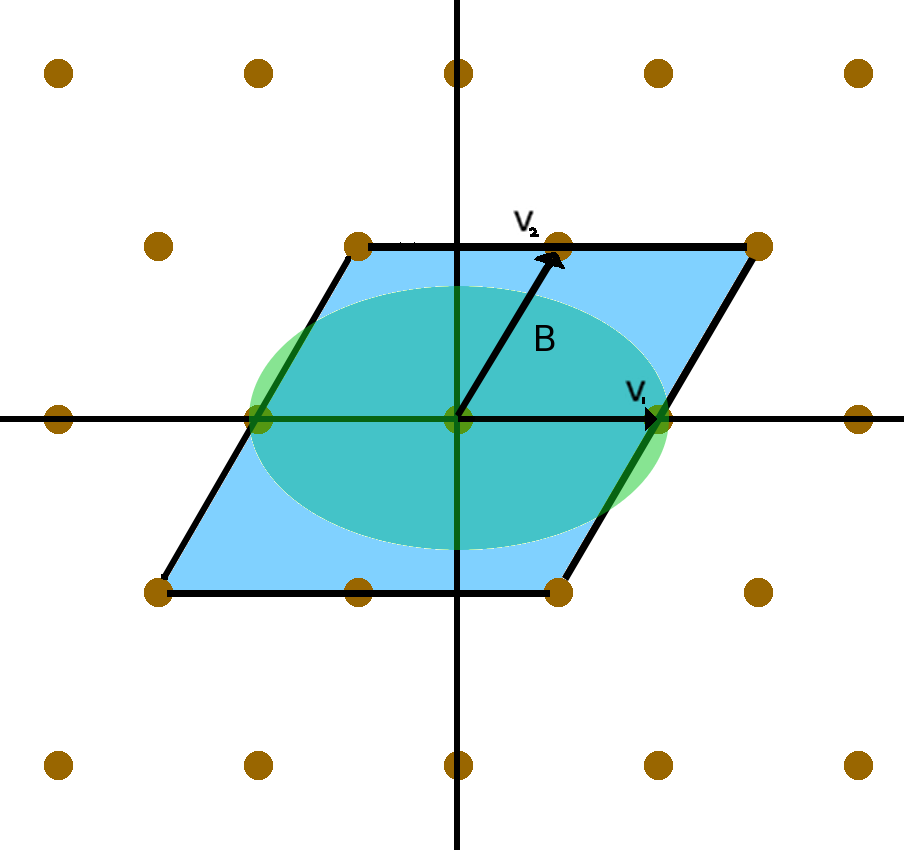
\includegraphics[width=2in]{Triangular_point_lattice}
\caption{Example \pgram{}s, $\L$, and $B$.}
\label{circlelattice}
\end{figure}

Looking at the plane (which is easier to visualize, as in Figure~\ref{circlelattice}), it is possible to make a \pgram{} that is just slightly smaller than 4 of the basic \pgram{}s tiled together and contains no nonzero lattice points. (The basic \pgram{} is just the one bounded by the basis vectors.) In $n$ dimensions, this is generalized to the \ptope{} with volume $2^n|\det(\vec v_1,\dots,\vec v_n)|$.

However, strange things can happen to the fundamental \ptope, since a lattice can have multiple $\Z$-bases. For example, $\left\{\binom{1}{0},\binom{0}{1}\right\}$ and $\left\{\binom{1}{1},\binom{1}{2}\right\}$ both represent the lattice $\Z^2$. A lattice is invariant under any change-of-basis matrix $T\in M_2(\Z)$ provided that $T^{-1}$ has integer entries. Thanks to some nice properties of $\Z$, this is equivalent to $\det T = \pm 1$, or that $T\in\GL{2}(\Z)$.
\begin{defn}
If $\{\vec v_1,\dots,\vec v_n\}$ is a $\Z$-basis of a lattice $\L\subset\R^n$, then a fundamental \ptope{} with respect to $\L$ is 
\[P = P_{\{\vec v_1,\dots,\vec v_n\}} = \left\{\sum_{i=1}^n t_i\vec v_i\mid 0\le t_i\le 1\right\}.\]
This \ptope{} and its translates cover $\R^n$.
\begin{claim}
All fundamental \ptope{}s of a given lattice have the same volume, called $\vol_{\L}$.\footnote{Notice this is not the volume \emph{of} $\!\L$, which is 0, because it is a discrete lattice.}
\end{claim}
\begin{proof}
Suppose $P$ is a fundamental \ptope{} corresponding to a basis $\{\vec v_1,\dots,\vec v_n\}$ for some lattice $\L$ and $P'$ is another fundamental \ptope{} corresponding to a basis $\{\vec v_1',\dots,\vec v_n'\}$ of $\L$. Then, there is some change-of-basis matrix $C$ such that $|\det C| = 1$. Then,
\[\vol P = |\det(\vec v_1,\dots,\vec v_n)| = |\det(C)\det(\vec v_1',\dots,\vec v_n')| = |\det C||\det(\vec v_1',\dots,\vec v_n')| = |\det C|\vol P' =\vol P'.\qedhere\]
\end{proof}
\end{defn}
\begin{thm}[Minkowski]
\label{mink}
Suppose $\L\subset\R^n$ is a lattice and $B\subset\R^n$ is convex and symmetric around the origin. Then, if $\vol(B) > 2^n\vol_{\L}$ (which is just $\vol_{2\L}$), then $B\cap(\L-\{0\}) \ne \emptyset$.
\end{thm}
Minkowski's Theorem is applicable to the four-square problem. Take $B_p = \{\|\vec v\|^2 < 2p\}\subset\R^4$ and $\L$ as given before, so that $\vol_\L = 2p^2$. In order for the theorem to be satisfied, we want $\vol(B_p) > 16p^2$. Using the four-dimensional volume of a sphere,
\[\vol B_p = \frac{\pi^2 (2p)^2}{2} = 2\pi^2 p^2 > 16p^2\]
because $\pi^2 > 8$. Step back and see how this number-theoretic property about squares of integers rests on this completly geometric property of $\pi$, which is totally unexpected.
\begin{proof}[Proof of Minkowski's Theorem]
Consider the region $2P = \left\{\sum_{i=1}^n t_i\vec v_i: 0\le t \le 2\right\}$, and for any lattice point $\vec m = \sum_{j=1}^n m_j\vec v_j$ define
\[D_{\vec m} = 2\vec m +2P = \sum_{j=1}^n 2m_j\vec v_j +2P\]
Thus, $D_{\vec m}$ is the \ptope{} translated so that one of the corners is at $\vec m$. Thus, its volume is constant, and $\vol(D_{\vec m}) = 2^n\vol_\L$. Additionally, they tesselate, since $\vec m$ is a lattice point: $\R^n = \bigcup_{\vec m\in\L} D_{\vec m}$, and they basically don't intersect (the intersections are hyperplanes with measure 0). Thus, $B\cap D_{\vec m}$ are also essentially disjoint, so since $B = \cup(B\cap D_{\vec m})$, then
\[\vol B = \sum_{\vec m}\vol(B\cap D_{\vec m}) > \vol 2P\]
by the original assumption. Now, it is possible to translate each of these pieces back to the origin, within the \ptope{} $2P$:
\[\implies \bigcup_{\vec m\in\L}(-2\vec m +(B\cap D_{\vec m})) \subseteq 2P.\]
\begin{figure}[h]
\centering
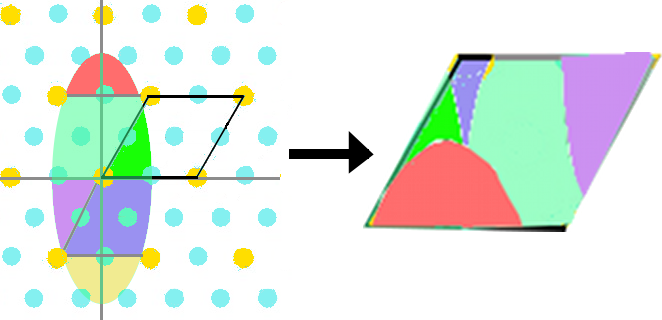
\includegraphics[height=2in]{lattice2}
\caption{Translating $B$ back to the origin to create an intersection.}
\end{figure}
But since these pieces have volume greater than $2P$, there must be distinct $\vec m$, $\vec m'$ with a nontrivial intersection: $-2\vec m + x = -2\vec m' + x'$, with $\vec m,\vec m'\in\L$ and for some $x,x'\in B$. Thus, $\frac{x'-x}{2} = \vec m'-\vec m$, which is also a nonzero lattice point (since $\vec m'$ and $\vec m$ are distinct) that is in $B$ (by symmetry, since $x$ is, then so is $-x$, and by convexity, their midpoint is as well).
\end{proof}
The four-squares theorem follows as above.
\end{proof}
A lot of problems in number theory, such as those relating to the theory of quadratic forms, can be solved in similar ways.
%a\end{document}

    \section{Game Theory, by Michael Manapat: July 18, 2012}
	Michael Manapat's trajectory through mathematics is unusual in that he went from very theoretical (number theory) to very applied (game theory, including working at Google).

\subsection{Evolutionary and Behavioral Game Theory}
The canonical game in the study of game theory is the Prisoner's Dilemma: cooperation comes at a positive cost $c$ to give someone else a positive benefit $b$.
\begin{defn}
A Nash equilibrium is a strategy such that if both players choose it, neither has an incentive to unilaterally defect to another strategy.
\end{defn}
Notice that in this game, defection is a Nash Equilibrium, but not cooperation! This is interesting, because the optimal outcome would be for neither to defect\dots{} but the optimal strategy for each person is to defect.

How often do people cooperate in this game? Most studies required recruiting people (especially undergrads) to play games. But undergrads are not representative of the general population. Recently, though, these sorts of studies have been implemented using Amazon's Mechanical Turk. Interestingly, there is little difference bewteen these methods: in each case, people cooperate roughly 40\% of the time.

So that means people don't behave rationally almost half the time. Why might that be? Several hypotheses exist. For example, intuitions about these things have developed in situations where they are repeated many times, which rewards cooperation.

One study created a Prisoner's Dilemma in which there was a probability of continuation after each game of 0.9. (This is more interesting than just fixing a number of times to repeat the game, in which everyone will cooperate, and then defect during the last game, since the incentive for cooperation is gone. But if you both know you'll defect on the last round, you'll defect on the round before, and by backwards induction, all the way to the first.) So in this probabilistic game, one could always defect or always cooperate, or choose more interesting strategies such as going randomly or alternating or such.

One strategy is called tit-for-tat, in which you cooperate the first round and follow the opponent's choice in round $n$ in round $n+1$. This has won tournaments and has a lot of nice properties. It also is aesthetically nice: it isn't vindictive. However, it actually tends to lose against most individual strategies, and is the overall winner because its overall average payoff is better. Moreover, it is rather predictable.

In the real world, tit-for-tat is not robust to errors (since in real life, mistakes in this sort of thing can happen). And this would cause switches from cooperation to defection, and result in somewhat random behavior over time. Thus, a better strategy is known as generous tit-for-tat (GTFT), which has a mechanism for detecting mistakes. These strategies actually occur in animal behavior.

This sort of strategy is known as direct reciprocity. One can also have indirect reciprocity (once described as based on names and reputation rather than faces) or network reciprocity (where reciprocity follows a network graph). Since the ability to recognize faces and names are different congitive abilities, these strategies should show up in different species. The continuation probability in each case is $w > c/b$.

\subsection{Game Theory in Computer Science}
Suppose Google has three slots for advertising space in a search and wants to distribute them to advertisers. Since Google is only paid if the ad is clicked, it wants to sell ad space that is also relevant to the search in question. Auction design is a setup that allows one to answer this problem.

\begin{defn}
A bidder $i$ has representation value $v_i$ if the bidder is never willing to pay more than $v_i$.
\end{defn}
The bidder wants to obtain the item and also maximize $v_i - p$, where $p$ is the winning price. But the auctioneer wants to sell the item for the highest price. Here game theory clearly is present.

One style of auction is the ascending (or English) auction, where the price is steadily raised until there are no further bids. This requires lots of communication and is unsuited for online advertisements; it requires too much coordination.

Alternatively, one could do a sealed bid. These bids will depend on others' assumptions and thus might not award the item to the person who wants it the most (or is even willing to pay the most).

\begin{defn}
A dominant strategy is a strategy which is optimal no matter the opponent's decision.
\end{defn}
In the Prisoners' Dilemma, defection is a dominant strategy. However, in a coordination game where it is favored to side with one's opponent, each strategy is Nash but neither is dominant.

The auctioneer wants to design the game such that bidding the representation value is the dominant strategy.

Truth-telling is a dominant strategy if bidder $i$ maximizes their payoff by bidding $v_i$ irrespective of the actual values of other players, $i$'s perceptions of these values, and the others' bids. In some sense, it should be best to play $v_i$ no matter the state of the world.

The solution is the Vickrey auction: a sealed-bid auction where the winner doesn't play their bid, but the second-highest bid plus some $\varepsilon$. Why does this work?

Consider two bidders. The expected payoff for the first is $(v_1-b_2)P(b_1>b_2)$ (where $b_i$ is the $i^{\mathrm{th}}$ bid). This favors setting $b_1=v_1$ in each case ($v_1 > b_2$, $v_1 < b_2$).

When there are multiple slots and there is one auction for several options, the first pays $\$1$ more than the second bid, the second pays $\$1$ more than the third, etc. However, since Google also cares about relevance, the bids are weighted by a quality score to judge whether ads will be clicked on.
\subsection{Decision Making}
Michael Manapat's life is a list of decisions between theoretical CS, pure math, and applied math, and between industry and academia. Do you want to go to grad school and work on a problem for five years? If so, maybe pure math is for you. If not, applied math might be better. But the results in pure math are also potentially worth it. Everything goes more slowly in pure math: years to learn a subject, years to publish, etc. But there's a lot of pressure to study pure math because anything else would be easier, and that's not necessarily a valid decision.

Similarly, academia versus industry is a choice that may be difficult. Within academia, there can be a notion that industry is lesser. There are plenty of more fulfilling or important things than necessarily becoming a mathematician. But there are advantages to both sides.

General advice by the lecturer: grad school isn't something you have to do. One can have an intellectually stimulating life outside of academia. Stanford's startup culture is nice for this. Additionally, it can be useful to learn probability and statistics. It can be useful in both pure and applied math. And, of course, figure out what you really enjoy.

    \section{Dispersal and Aggregation, by Dr. Nancy Rodriguez: July 25, 2012}
	In some sense, PDEs are considered more applied than pure, but it's not terribly different: lots of functional analysis is involved.

A reaction diffusion system is a system of particles (which can be used to model animal or human populations) given by the equation $u_t = \D u + f(u)$. The Laplacian corresponds to the diffusion and $f$ measures the reaction.

A related type of PDE is a reaction diffusion advection, of the form $u_t = \D u + f(u) +\nabla(u\nabla \vec v)$, in which the last term represents moving the system under $\vec v$, and is called an advection.

Generally, these are referred to as evolutionary equations, since they often deal with questions relating to the change of a system over time.

Since these are PDEs, it is difficult or explicitly impossible to find explicit solutions, so qualitiative analysis is more common. One might ask questions of existence or uniqueness of solutions, whether the model blows up in finite time (which would imply it's not a great model for population biology), what its long-term behavior is, and whether any patterns exist.

These sorts of equations have applications to modelling nonlocal biological aggregation (such as schools of fish), and in particular chemotaxis.\footnote{Chemotaxis is the influence of a chemical substrate in the environment on the movement of some mobile species, typically a protist.} The diffusion is generated by a desire for personal space, and the aggregtion by some desire to group together. Interestingly, this movement does not have any leader.

For example, the slime mold \emph{Dictyostelium discoidum} follows this model: one individual secretes cAMP, and others are attracted towards it and secrete some of their own. However, secretion happens only once every six minutes and the amoeba move only for about 60 seconds before stopping. Thus, the amoeba diffuse, but also move towars the chemo-attractant.

\begin{defn}
The convolution of two functions $\cK$ and $u$ is
\[\cK * u = \int_{\R^n} \cK(x-y)u(y)\ud y.\]
\end{defn}

The overall group behavior model is
\[u_t = \D A(u) - \nabla \cdot (u\nabla \cK * u),\]
where $\D A(u)$ models the dispersal and $\nabla \cdot (u\nabla \cK * u)$ represents the aggregation. In some cases, the aggregation wins; in others, the dispersion does.

Consider the heat equation for $u(x,t)$: $u_t = \nabla(D\nabla u) = D\D u$ where $D$ is some diffusive coefficient. One of many ways to solve it is to take the Fourier transform to get
\[\dfr{}{t} \hat u(\xi,t) = -D|\xi|^2\hat u(\xi,t),\] which is ordinary and thus can be solved explicitly:
\[u(x,t) = \frac{1}{(4\pi t)^{n/2}}\int_{\R^d} e^{-\frac{|x-y|^2}{kt}} u_0(y)\ud y = \Phi(x,t) * u_0(t),\]
where $\Phi = e^{-\frac{|x|^2}{kt}}$ is called the heat kernel.

This solution in some sense averages the values of the initial data, because for initial data with compact support, the support for any positive $t$ will be $\R^n$. Diffusion happens with instantaneous speed (called infinite speed of propagation), which is obviously not a good model for the real world.

A potential solution is to introduce an overcrowding effect, which makes diffusion stronger in denser areas. In this case, the equation is
\[u_t = \D A(u) = \nabla\cdot(A'(u)\nabla u),\] where $A'(t) \to 0$ as $u\to 0$ and is eventually linear (degenerate diffusion). In this case, $A'(t)$ stands in for the diffusivity coefficient.

In physics, the porous medium equation is used to model gases: $A(u) = u^m$, where $m> 1$.\footnote{If $m = 1$, then fast diffusion and infinite speed of propagation happen.}

The heat equation does have some solutions which have compact support and finite speed of propagation, such as Baerblatt's solution, which is also scale-invariant:
\[u(x,t) = \frac{1}{t^\alpha} \left(b - \frac{(m-1)\beta|x|^2}{2mt^{2\beta}}\right)^{\frac{1}{2m-1}}\]
However, this equation is not smooth at the boundary, so there are no classical solutions and it's not a good model to work with.

One way to get around this is to generalize the notion of a derivative. Weak differentiation involves finding some $\varphi\in C^\infty$ such that $\int u\dfr\varphi t +\int u\dfr \varphi u = -\nabla u\nabla \varphi +f(u)\varphi$, and solutions to differential equations obtained in this method are called weak solutions.

One simple way to model aggregation is to add a factor in the direction $\nabla u$, since this is the direction of steepest increase. For example, the transport equation represents the transportation of some fixed quantity: $\rho_t+\nabla \cdot(\rho\vec v) = 0$. This is fairly simple and nice, but there are no nonlocal effects. Thus, a better model would replace $\nabla u$ by
\[\nabla \cK*u =\int_{\R^d}\nabla\cK(x-y)u(y)\ud x\] for some kernel $\cK$. For example, one could use the Newtonian potential
\[\mathcal{N}(x) =\left\{
\begin{array}{l l}
-\frac{1}{2\pi}\log|x| & d = 2\\
c_d|x|^{2-d} & d > 2.
\end{array}
\right.\]
Thus, the question becomes: for some kernel $\cK$ which measures aggregation, how much diffusion is necessary to prevent a finite-time blowup?

In order to analyze this, it is first necessary to establish some properties:
\begin{enumerate}
\item Conservation of non-negativity: if $u_0 \ge 0$ and $t > 0$, then $u_t > 0$.
\item Conservation of mass: $\dfr{}{t}\int u(x,t)\ud x = 0$.
\end{enumerate}
There is also a free energy functional that indicates the final behavior of the system:
\[\cF(u) = \int\frac{u^m}{m-1}\ud x - \frac{1}{2}\int u(x)u(y)\cK(x-y)\ud x\ud y.\]
This can be rewritten as $\cF(u) = S(u) - W(u)$, where $S(u) = \int \frac{u^m}{m-1}\ud x$ is the entropy, which favors diffusion, and $W(u) = \frac{1}{2}\int u(x)u(y)\cK(x-y)\ud x\ud y$ is the interaction energy, which favors aggregation.
\begin{prop}
Weak solutions to the aggregation diffusion equation satisfy the energy dissipation inequality
\[\cF(u(t)) +\int_0^t\!\!\!\int\frac{1}{u}|A'(u)\nabla u - u\nabla\cK * u|^2\ud x\ud t \le \cF(u_0(x)).\]
\end{prop}
The proof is a straightforward plug-and-chug, though it does involve integration by parts.

Consider a mass-invariant scaling $u_\lambda(x) = \lambda^d u(\lambda x)$. As $t$ increases, $u$ scales into a delta function. Consider $\cF = \mathcal N$ and $d\ge 2$: as $u\to\delta$, both $S(u)\to\infty$ and $W(u)\to \infty$. However, the state of the system (and whether diffusion or aggregation will dominate) depends on which does so faster.

The key quantity is $m^* = \frac{2(d-1)}{d}$. When $m > m^*$, then the $\delta$-function is not a minimum for $\cF$, so entropy dominates; there is global existence of a solution. If $m < m^*$, then the $\delta$-function does minimize energy, so the solution converges to it ---  and blows up in finite time.

If $m = m^*$, more interesting things happen. The problem then comes down to the initial mass. If $M < M_C$ for a certain critical mass $M_C$, then there will be global existence; if it is strictly greater, then the solution will blow up. In general, it is unknown what happens when $M = M_C$; it may well depend on some other critical factor.

In the more general case, there is a notion of criticality.
\begin{center}
\begin{tabular}{l r c c l}
subcritical: & $\displaystyle{\liminf_{z\to\infty} \frac{A'(z)}{2^{m^*-1}}}$ &$=$ &$\infty$ & does not blow up;\\
critical: &$\displaystyle{\liminf_{z\to\infty} \frac{A'(z)}{2^{m^*-1}}}$ &$<$ &$\infty$ & depends on critical mass;\\
supercritical: &$\displaystyle{\liminf_{z\to\infty} \frac{A'(z)}{2^{m^*-1}}}$ &$=$ &0 & blows up.
\end{tabular}
\end{center}

    \section{Earthquake Cycle Simulations, by Dr. Brittany Erickson: July 30, 2012}
	Dr. Erickson is in the interesting position of being a postdoc in the geophysics department despite having a PhD in mathematics. Her work relates to the mathematical modeling of earthquakes.

The San Andreas Fault is a vertical strike-slip fault (the two sides move past each other, instead of causing subduction). One way to model this is in a lab, pushing rocks against each other at high pressures.

The Burridge-Knopoff model is a way to model a block attached to a spring with some law of friction: the friction stress statisfies $\tau = \mu\sigma_n$ (where $\sigma_n$ is the normal stress and $\mu$ is a nonconstant coefficient of friction). $\mu$ is logarithmically dependent on sliding velocity and a state variable (which accounts for the irregularity of the surface). It can be quite difficult to account for the variability of these such variables over time or scale them up to faults.

This model doesn't seem to have an analytic solution, but there are two solutions: the stationary situation has all time derivatives equal to 0; the block just slides along. But periodic solutions also exist, in which the block gets stuck and then shoots forward periodically. This is called stick-slip behavior, and the jerks forward actually correspond to earthquakes.

A more complicated model involves viewing the fault in 3-dimensional space. Temperature is also accounted for (since deeper into the Earth, movement is easier than at the top). In order to simplify the model, it can be discretized and a couple assumptions need to be made: such as that the earth around the fault is perfectly elastic (which seems untrue).

Then, using Newton's Second Law, one can set up a system of PDEs in $\R^2$: $\rho\ddot u = G\nabla u$ (where $u$ is the displacement and $G$ is a modulus that represents stiffness). There will thus be some boundary conditions given by the shear stress.

Solving semi-discrete equations is actuall how PDEs are solved numerically, so chopping up this PDE results in a huge system of (non-differential) equations. This ends up being approximately $u_{tt} = Ku$ for some matrix $K$ (plus some boundary conditions). This equation is an ODE now, which makes solving by computer a bit easier.

One area of research is to try and model the initial conditions before an earthquake, or to model the entire earthquake cycle. This can be computationally intensive, but some simplifications can be made. In particular, the acceleration is nearly zero, so $0 = G\nabla u$, which makes the computation much less difficult. This results in a periodic model rather like the simpler one, in which the velocity is very slow for most of the time and then large (1 meter per second) during earthquakes. The shear stress builds up over time, until it is released with each earthquake. Notice that this periodicity doesn't happen very often in real life, but that can be represented by a fault that's not a line or making the initial stress heterogeneous.

Another way to add complexity to the models is to notice that permanent damage and change can happen after earthquakes, changing the nature of the rocks around it. There is a core of highly damaged rocks, and farther from the fault less and less damage and more elascitity (which lends an ability to recover from damage, like Play-Doh). Rocks, however, are both elastic and plastic: they can be bent to a degree, but eventually can't return to their initial state if subjected to a sufficient amount of stress.

Interestingly, it is better to know how an earthquake will happen rather than when, since designing earthquake-safe buildings is so helpful. Thus many seismologists predict that it will be possible to predict ground motion eventually, but not necessarily the timing of earthquakes.

Plasticity is a constrained optimization problem. The set of admissible stresses is $\mathbb E = \{\sigma_{ij}:f(\sigma_{ij}) \le 0\}$ ($f$ is the yield condition) and the flow rule requires $\dot\epsilon = \lambda P_{ij}(\sigma_{ij})$ (where $\epsilon$ is a second-order tensor), etc. It can be difficult to include these laws in a model, so sometimes some are left out. There is an elastic stiffness tensor that is fourth-order and not particularly fun to play with, but they are solved through an iterative procedure. These large nonlinear systems can be solved through fixed-point methods, Newton's Method, and other such numerical methods.

(The next earthquake in the Bay Area is predicted to be along the Hayward fault, in the East Bay, sometime in the next 30 years. It is estimated to be magnitude 6 or so --- not much greater. But the Pacific Northwest is overdue for a big one, and that's a subduction zone, which means it might be much stronger.)

    \section{Some Differential Geometry, by Dr. Rafe Mazzeo: August 1, 2012}
	%WHere are your pictures?
Consider some manifold $M^n\subset \R^N$ with some metric $g$. Consider the tube of radius $r$ around this manifold:
\[T(r) :=\{x\in\R^N:g(x,M) = r\},\]
which is a manifold of codimension 1. This tube is in a sense the product $M \times S^{N-n-1}$, though if $M$ is not completely straight this is incorrect. However, it is roughly so, since the volume $V(r) = \vol(T(r)) \sim r^{N-n-1}$.

More explicitly, Weyl's Tube Formula gives the volume as polynomial in $r$: $V(r) = \sum_{j=0}^{N-n-1} a_jr^j$, where the $a_j$ are geometric invariants. $a_0 = \vol(M)$, which is a geometric qualtity, but $a_{N-n-1} = \chi(M)$, the manifold's Euler characteristic, which is topological.

In $\R^3$, this simplifies to $V(r) = \chi(M)r^2 + \Area(M)$ for a surface and $V(r) = 2\pi r\ell(M)$ for curves. This latter case is interesting because it looks exactly like if the tube were the direct product $M\times S^{N-n-1}$.

This model has some interesting and unexpected applications in statistics.

Differential geometry also uses hyperbolic space. One can think of hyperbolic space $\H^n\subset \R^n$ as an open disc in which lines in $\H^n$ are arcs of circles in $\R^n$ and parallel lines are defined as those that do not intersect. Thus, one line can have many parallels, some of which intersect each other.

The Riemannian metric for hyperbolic space is
\[g = \frac{\sum_{i=1}^n \ud x_i^2}{\left(1- \sum_{i=1}^n x_i^2\right)^2},\]
which results in a constant curvature of $-1$. it also leads to a Laplacian, which is different from $\D g_{_{\R^n}} = \sum_{j=1}^n \frac{\partial^2}{\partial x_j^2}$. However, it enables one to think of bounded harmonic functions in $\H^n$.

Liouville's Theorem states that any bounded harmonic function in $\R^n$ is constant, but hyperbolic space (which is topologically just an $n$-dimensional space) looks very different; there are plenty of nonconstant harmonic functions, and any continuous function on ``the sphere at infinity'' is the limit of some harmonic function. This is indicative of the different geometries of $\R^n$ and $\H^n$, which is also represented by the fact that the volume of the unit ball in $\H^n$ grows exponentially with the radius, rather than as a polynomial.

Instead of considering strictly harmonic functions, however, one can consider solutions to the equation $(\D + \l^2)u = 0$ in $\R^n$, which have applications to scattering theory in mathematical physics. Looking from infinity, $u$ will satisfy the Helmholtz equation
\[
u \sim r^{\frac{1-n}{2}} e^{i\l r}a(\theta) +r^{\frac{1-n}{2}}e^{-i\l r}a(-\theta)
\]
where $\theta\in S^{n-1}$ and $a$ is some function. Physically, this means sending waves through Euclidean space doesn't change them; they come out like they went in. However, if you add some obstacle $K$, an additional requirement of $u|_{\partial K} = 0$ as well. This is similar, but the equation then becomes
\[
u \sim r^{\frac{1-n}{2}} e^{i\l r}a(\theta) +r^{\frac{1-n}{2}}e^{-i\l r}b(\theta)
\]
for some other function $b$. Physically, this means the waves will get scattered by the obstacle $K$, and this equation can be backed up by physical data. Given scattering data, what can one determine about $K$? This problem has applications in seismology, oil detection, etc. Additionally, one can study the scattering operator for this system, given by $b = S(\l) a$.

This has applications in, of all places, number theory. Consider the modular surface $\H^2/\SL{}(2,\Z)$. This looks like a once-punctured torus with a cusp at infinity, and has constant negative curvature. This surface has a hyperbolic Laplacian associated with it, and let $S(\mu)$ be the scattering operator for the equation
\[\left(\D g +\left(\frac{1}{4} +\mu^2\right)\right)u = 0.\]
Looking from the cusp at infinity and sending a wave in, it will reemerge with some function that determines $S$. Considering $\mu\in\C$, $S$ will have poles, whose location is determined by the Riemann Hypothesis.

    \section{Hopf Algebras and {\sc Sage}, by Dr. Daniel Bump: August 8, 2012}
	\subsection{Hopf algebras}
The motivation behind a Hopf algebra is to define a group in terms of mappings in a way that can be abstracted to other things. In this formalism, a group $G$ has an operation $G\times G\stackrel{m}{\to} G$ called multiplication and two homomorphisms $1\stackrel{\e}{\to} G$ (the unit) and $G\stackrel{\e^*}{\to} 1$ (the counit). These latter two operations are equivalent to the identity axiom.

Associativity is given by the commutativity of the following diagram:
\begin{equation}
\label{assoc}
\xymatrix{
G\times G\times G \ar[r]^{\ m\times 1} \ar[d]^{1\times m} & G\times G\ar[d]_m\\
G\times G \ar[r]^m & G.
}
\end{equation}
But this doesn't add any information about inverses, so let $S:G\to G$ be given by $S(x) = x^{-1}$ and let $G\stackrel{m^*}{\to} G$ be the diagonal map $x\stackrel{m^*}{\mapsto} (x,x)$, called comultiplication. Then, the inverse property is equivalent to the commutativity of
\begin{equation}
\label{inverses}
\xymatrix{
G \ar[r]^{m^*} \ar[d]^{\e^*} & G\times G \ar[r]^{1\times s} & G\times G \ar[d]^m\\
1 \ar[rr]^{\e} & & G
}\end{equation}
and of the analogous diagram for $s\times 1$.

As an example, this can be used to say things about vector spaces using tensor products. The universal property of the tensor product is that for vector spaces $V,W$, $V\times W$ is equivalent to $V\otimes W$ under the map $(x,y)\mapsto x\otimes y$. Thus, the properties of vector spaces can be reformulated in terms of tensors, including equivalents of diagrams \ref{assoc} and \ref{inverses} but with $\otimes$ substituted for $\times$, as well as some other properties. Thus, one could develop group theory as a special case of Hopf algebras.

In this formalism, the significance of comultiplication is that if $V,W$ are modules of a Hopf algebra $H$, then $V\otimes W$ is also a module, since $h(v\otimes w) = m^*(h)(v\otimes w)$ in $H\otimes H$.

It would be nice to have $V\otimes W \cong W\otimes V$. One possibility is the map $\tau:x\otimes y\mapsto y\otimes x$, but this sometimes doesn't work, and the map needs to be $\tau R$ for some $R\in H$. This map must be an isomorphism, and it also must satisfy the Yang-Baxter equation:\footnote{Interestingly, both of these are physicists; the equation itself initially came out of mathematical physics.} $R_{12}R_{13}R_{23} = R_{23}R_{13}R_{12}$ in $H\otimes H\otimes H$, where $R\in H\otimes H$ gives $R_{ij}\in H\otimes H\otimes H$ by placing $R$ in positions $i$ and $j$. Thus, $R_{12} = R\otimes 1_H$ and $R_{23} = 1_H \otimes R$, and if $R = \sum_{\alpha = 1}^N S_\alpha \otimes T_\alpha$ for $S_\alpha,T_\alpha\in H$, then $R_{13} = \sum_{\alpha = 1}^N S_\alpha \otimes 1\otimes T_\alpha$.

Consider three modules $U,V$, and $W$.
\begin{equation}
\label{isohexanol}
\xymatrix{
& V\otimes W\otimes U \ar[ld]_{\tau R\otimes 1} \ar[rd] &\\
W\otimes V\otimes U \ar[d] && V\otimes U\otimes W\ar[d]\\
W\otimes U\otimes V \ar[rd] && U\otimes V\otimes W\ar[ld]\\
& U\otimes W\otimes V &
}
\end{equation}
The Yang-Baxter Equation says that the left-hand and right-hand sides of Diagram~\ref{isohexanol} are identical isomorphisms.
\subsection{{\sc Sage} and Hopf algebras}
A lot of the calculations involving Hopf alegbras can be done with \textsc{Sage}, in part because Dr. Bump has contributed code to the project! However, not all of the code is in a stable release, as demonstrated when the program accidentally redefined $e$.

Consider some group \texttt{G = CyclicPermutationGroup(7)} (i.e. $\mathtt G = S_7$) and let $\mathtt H$ be the Hopf algebra over $\mathtt G$ (which is done with the command \texttt{H = GroupAlgebra(G)}). \textsc{Sage}'s notation can be a bit counterintuitive; \verb+#+ is used for $\otimes$, and \texttt{()} is used to repreent the identity (which was sufficiently confusing that Dr. Bump decided  to write a wrapper class around it to fix it). Thus, if $\mathtt g$ is the group generator, then the command \texttt{(1+g).coproduct()} returns \verb!1 # 1 + g # g!, which is akin to saying $m^*(1+\mathtt g) = 1\otimes 1+\mathtt g\otimes \mathtt g$.

Consider $R = \sum_{g\in \mathtt G} q^{-ab} g^a\otimes g^b$, where $q = e^{\frac{2\pi i}{n}}$ is an $n^{\mathrm{th}}$ root of unity. This should satisfy the Yang-Baxter equation as well as some more interesting properties, which can all be tested in \textsc{Sage}. (Generating $R_{13}$ is a little more interesting, but can be done with the map $\mathtt H\otimes \mathtt H \stackrel{\mathtt f}{\to} \mathtt H\otimes \mathtt H\otimes \mathtt H$ given by $\mathtt f:x\otimes y \mapsto x\otimes 1\otimes y$. Though this isn't terrifically complicated, it can be simplified into one line using Python's lambdas.)

For further reference, the book Majid, \textit{A Quantum Groups Primary} might be interesting or useful.

    \section{The Shape of Data, by Dr. Gunnar Carlsson: August 13, 2012}
	For these purposes, data is a point cloud (a finite set of points in some Euclidean space). Sometimes, though, as in DNA sequences, data isn't strictly a point, but rather a sequence. In ither case, a distance metric exists: the usual distance metric in Euclidean space, and the Hamming distance for sequences, which measures by how many points a sequence differs. Distance can be used to represent data, which leads to a notion of shape.

Shape of course is very relevant to data. For example, the most primitive notion of shape is whether the data clusters, which admits important statistical consequences. In general, shape represents some connected components; $\pi_0(x)$ denotes the set of connected components.
\begin{figure}[h!]
\centering
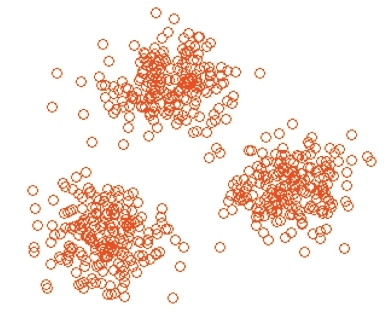
\includegraphics[width=2in]{clustering}
\caption{An example of data clustering into 3 different clusters.}
\end{figure}
Shape can also take the form of loops or other devices that represent periodic or recurrent behavior (as in the Lodka-Volterra predator-prey model), denoted $\pi_1(x)$ or $H_1(X)$, or flares, which indicate different ways in which the data can be an outlier, denoted $\pi_0^\infty(x)$.

In topology, one constructs invariants that measure this sort of shape. For $\pi_0(x)$, choose some distance $R$ and build a network (or simplicial complex; fill in all possible triangles, tetrahedra, etc.) connecting any two points with distance less than $R$. This actually builds up connected components from discrete sets, but distance must be chosen with care, or one obtains too many or too few clusters; choosing the proper $R$ can be an art. In statistics, heuristics exist, but there are plenty of counterexamples that limit their validity. However, a dendrogram (see Section~\ref{dendrogram}) can be helpful here.

Let $V(X,R)$ be the simplicial complex such that $x_i,x_j\in X$ are connected iff $d(x_i,x_j) \le R$. Thus, for every $R$, there is a set $\pi_0(V(X,R))$ of connected components at that fineness. If $R'<R$, then there exists a map $\pi_0(V(X,R))\to \pi_0(V(X,R'))$ because the latter is a subcomplex of the former (in a sense, it's more difficult to be a complex in $R'$). Thus, one can draw maps and points, leading to the familiar notion of a dendrogram. if the number of components remains constant over a long distance, then that suggests a correlation worth investigating.

Anothr method of doing this involves a homological method of shape. For every $k\ge 0$ and space $X$, one can associate a vector space on $\mathbb F_2$\footnote{$\mathbb F_2$ is sometimes called the Boolean space because its addition operation is equivalent to logical \texttt{xor} and its multiplication to logical \texttt{and}.} $H_k(X)$ such that $\dim H_k(X) = \beta_k$, where $\beta_k$ is the $k^{\mathrm{th}}$ Betti number.

$\beta_0$ is the number of connected components in $X$, and $\beta_1$ is the number of independent loops in $X$, so, for example $\beta_1(S^1) = 1$, and the first Betti number of two circles joined at a point is 2. Similarly, $\beta_1(T^2) = 2$, since there are two independent loops, but $\beta_1(S^2) = 0$, since all loops on $S^2$ can be shrunk to a point. Though these seem imprecise, rigorous foundations exist, and Betti numbers can be computed with methods from linear algebra.

%Have you added pictures yet?
$H_k$ is functional in that if $f:X\to Y$ is continuous them $H_k(X)\to H_k(Y)$ is an induced linear map. Apply it to $V(X,R)$, since the Betti numbers can change as $R$ imcreases (both increasing and decreasing; when nine points are separate, $\beta_1 = 0$, but when they become homeomorphic to a circle, $\beta_1 = 1$. When they are all connected again, $\beta_1 = 0$ again). In particular, for incomplete data, the Betti numbers might notice gaps or otherwise return the wrong result. Thus, one can do something similar and let $W_R = H_1(V(X,R))$ (some vector space over $\mathbb F_2$ and $W_R\to W_{R'}$ when $R < R'$ (due to the functoriality of the homology construction), which makes it necessary to find invariants on these persistence vector spaces.

These persistence spaces can be classified by ``bar codes'' (finite numbers of intervals). The category of persistence vector spaces happens to be equivalent to a certain category of rings for which an analogue to the Fundamental Theorem of Modules over Principal Ideal Domains (a generalization of Theorem~\ref{fgagtheorem}) holds, so some algebra comes over to help. If the barcodes contain  particularly long intervals, one can use them to classify things that are likely to be more meaningful. This is analogous to the dendrogram but involves loops rather than clustering.

One can apply this to statistics, but care must be taken --- it isn't practical for sufficiently complicated data sets, and point clustering may be ineffective. However, one can study similar problems or subproblems. For example, it is incredibly difficult to study all images of a given size, but one can study $3\times 3$ patches of images. Further refinement can be made because most pictures are dominated by constant patches, which can easily be removed. Thus, one looks at high-contrast patches of images that are normalized with respect to the mean (for intensity) and the $L^2$ norm (which represents contrast). This set $\mathcal M$ is dense in $S^7$, which is a little easier to work with. However, the density varies. This can be estimated (generally by counting the number of data points in a ball of a certain radius). If one considers the 25\% if the sphere with the largest density, there are always 5 intervals in the bar code, which was unexpected. However, this does correspond to a three-circle structure, with a primary circle that intersects two secondary circles (which do not intersect each other).

In order to simplify the problem further, one can represent this on a 2-dimensional surface: the Klein bottle. One can construct probability distributions and therefore Fourier analysis on the Klein bottle, which makes processing information nice. Thus this abstract Klein bottle can be used for very concrete applications.

    \section{Mathematical Doodling, by Dr. Ravi Vakil: August 15, 2012}
	%Where are your pictures?
In some sense, the difficulty of research is asking the right questions, and in ways which can be considered elegant.

%Pic here
Suppose one draws a doodle around a bunch of letters. Do successive doodles get more circular? What does that even mean mathematically?
\begin{defn}
For some plane set $X$, define the $r^{\mathrm{th}}$ neighborhood (or $r^{\mathrm{th}}$ doodle) of $X$ to be $N_r(X) = \{y:|y-x|\le r\text{ for some }x\in X\}$.
\end{defn}
Thus, in what sense does $N_r(N_r(\dots(N_r(X))\dots))$ become ``more circular?''

How does a choice of $r$ affect the situation? (In this methodology, math, both pure and applied, is an experimental science, made by hypotheses rather than dry exposition by theorem-proof.)
\begin{claim}
$N_{a+b}(x) = N_a(N_b(X))$.
\end{claim}
\begin{proof}
First, to show that $N_{a+b}(X) \supset N_a(N_b(X))$, anything that can be reached by a step of length at most $a$ from $X$ followed by a step $b$ must be reachable by a step of at most $a+b$ by the Triangle Inequality.

Conversely, if something can be reached by a step of at most $a+b$, it can be reached by a step of at most $a$ followed by a step of at most $b$ (just going in the same direction).
\end{proof}
Thi claim could even be thought equivalent to the Triangle Inequality, and used as a definition that is investigated on generalizations on spheres and such.

Then, as $r\to\infty$, does $N_r(X)$ become more circular? It does, thanks to the obvious observation that if $A\subset B$, then $N_r(A) \subset N_r(B)$:

Let $p\in X$ be in some sense its center and let $C_t$ be the circle of radius $t$ around $p$. Pick some $r$ such that $X\subset C_r$. Then, $\{p\}\subset X\subset C_r$, so
\[C_R = N_R(\{p\})\subset N_R(X)(C_r) = C_{R+r}\]
for some $R$, and as $R\to\infty$, $N_R(x)$ is caught between two circles that approach each other.

Thus, the definition of ``more circular'' is given \emph{after} it is proven --- which seems irrigorous, but is in line with the experimental approach.

%A picture would be nice here too.
Now consider the perimeter and area of these sets. If $X$ is a convex polygon, let $P$ denote perimeter and $A$ denote area. Since $X$ is a convex polygon, $N_r(X)$ is nice: it is $X$ with its edges extended out a distance $r$, and the remaining area filled in by circular arcs. The total angle of the arcs is $2\pi$, so $P(N_r(X)) = P(X) +2\pi r$.

The area argument is exactly the same, and $A(N_r(X)) = A(X)+P(X) + \pi r^2$.\footnote{It is no coincidence that $\frac{\ud A}{\ud r} = P$; think about why this might be.} This is a quadratic polynomial in $r$ --- its coefficients have a more interesting meaning than just appears on the surface.

Now generalize further: suppose $X$ is a general convex region. Using the normal vector (i.e. the vector perpendicular to the tangent vector to $\partial X$, oriented outward), the same formulas for perimeter and area hold, thanks to Green's Theorem.

Suppose the Earth is a perfect sphere and that a string is wrapped tightly around it. If the string's length is suddenly increased by 1 meter, how high up would it have to be to be taut again? The answer is $1/2\pi$ meters, which is much more than anyone expects. In particular, it doesn't depend on the radius or even the shape of the Earth, only that it is convex.\footnote{So, yeah, about that\dots but it's still a close enough approximation, since one could always just consider the convex hull.} If $X$ is a cross-section of the Earth, then the string is $N_r(X)$, and $P(N_r(X)) - N_r(X) = 1$. Solving for $r$ yields the correct answer.

If convexity isn't important to you, the formula can still hold; however, perimeter and area may have to be redefined for this to work (implying the new, less intuitive definitions are more ``natural''). In particular, the area of $N_r(X)$ must double-count separate parts of the doodle that overlap, and must ignore the holes.

However, some strange things happen. A figure 8 has $P(N_r(X)) = P(X)$, and other surfaces have $P(N_r(X)) - P(X) = 2\pi r$ (once again, the notion of area must be closely defined; in these cases it is signed, taking orientation into account).
\begin{defn}
The winding number of some curve around a point is the signed number of turns around that point that it makes.
\end{defn}
Thus, the winding number affects the perimeter and area. All the convex examples had a winding number of $1$; the figure $8$ has a winding number of $0$.

Another option is to add holes or make $X$ disconnected. Then, $A(N_r(X)) = A(X) +nP(X) +\chi(X)\pi r^2$, where $\chi(X)$ is the Euler characteristic, a fundamental topological invariant that is the number of disconnected pieces minus the number of holes.\footnote{For the perimeter, just take the derivative.} This is one of many remarkable mathematical examples that relate the continuous and the discrete.

One can gneralize yet again to higher dimensions. For example, something similar happens in three dimensions. If $V$ is the volume and $A$ the surface area, then
\[V(N_r(X)) = V(X) + A(X)r +(h+\ell+w)\pi r^2 +\frac{4\pi r^3}{3}.\]
The quadratic term is new, however, and is often forgotten in the generalization. But how does it generalize? What does it represent?

Consider a Russian train company with a rule that no package can be allowed with a total $\ell+w+h > 1$. Is it possible to encase one package inside another to get around this rule (e.g. diagonally)? As it happens, no.\footnote{``One thing you learn about mathematics is, if you ever get into an argument with a Russian, then the Russian wins.''} If $X\subset Y$, then $V(N_r(X)) \le V(N_r(Y))$. Letting $r\to\infty$, the quadratic term dominates, so $h_y+\ell_y+w_y > h_x+\ell_x+w_x > 1$.

In $n$-dimensional space, if $X$ is some convex region, these invariants are very interesting. In this case, $V(N_r(X)) = \sum_{i=1}^n k_i(X)r^i$, where $k_0 = V$ (the hypervolume), $k_1$ is the hypersurface area, and $k_n$ is the volume of the unit $n$-sphere.

The set of compact orientable surfaces of genus $g$ has a structure as a vector space of dimension $6g-6$. It has both a size and a shape (i.e. a topology). Witten conjectured up an algorithm for this related to representation theory (and inspired by string theory), which was later proven by others. Eventually, the P.h.D. thesis of Miriam Mirzekhani, a Stanford professor, generalized this to surfaces with holes in them (as opposed to just handles that affected the genus). If the sizes of the holes are fixed, the surfaces still form a vector space, with a volume completely analogous to the polynomial expression for $V(N_r(X))$, and it can be determined through topological techniques called cutting, pasting, and sewing. This also leads to another proof for Witten's conjecture.

A related Hilbert problem: is it possible to dissect a cube into a finite number of pieces (\emph{without} Banach-Tarski) and rearrange them to form a pyramid? In two dimensions, this is easy; area is the only invariant under dissection. But in three dimensions, there are two invariants: volume and a new volume-like invariant. Then, there are more and more in higher dimensions.

This three-dimensional invariant is related to the shadow cast by the object onto a plane\dots which means it has been applied to determine the surface areas of transiting exosolar planets!

\chapter{Lectures About Research}
    \section{Effective Mentor-Mentee Relationships, by Brian Thomas: June 29, 2012}
	%\documentclass{amsart}
%\usepackage{geometry,microtype,hyperref}
%\geometry{margin=1in}
%\begin{document}
%\title{The Importance of the Mentor-Mentee Relationship}
%\author{Brian Thomas\\\today}
%\maketitle
Though mentors take many forms (grad students, postdocs, professors, etc.), they all operate in similar ways. They key is that on both sides of the relationship, there are human beings on both ends. Sometimes this gets forgotten. Basic human social interactions are often the reason such relationships succeed or fail.\footnote{Wait, is this a talk on social skills for math majors?}

Consider two types of mentorship (see handout). One extreme is the professor who is very obvious about what sort of direction and timeline the mentee would take, and the other is someone who is much more laid-back. Though most people fall in the middle, the latter type tends to be attracted to academia.

A lot of people prefer this latter type of professor, due to their open-endedness and lack of pressure. Of course, a more structured research project has advantages too; you will probably learn more.

Another important question is despite which is preferable, which would make for more productive research? I personally believe the answer is somewhere in the middle, but there are advantages to the structured approach.

Given that professors are somewhat immutable in this regard, you have to think about this explicitly and know what's going on in order to set a good relationship. Thus, good mentoring relationships can be designed. This is the sort of thing that one must do early and figure out ahead of time --- establish what is expected and what preconceived notions exist.

So, how can this happen? Consider a student who wants to work in a more self-directed manner under a professor who is more directed. This could cause tension about different interests. For example, some students are just interested in experiencing research, but the professor wants to see a paper. If this sort of collision is addressed early, it can be rectified. So, consider: if you had a half-hour meeting on addressing expectations (i.e. you should do this), what topics would be discussed? The final product, the frequency of interaction (which is different for each research project), which direction the research should take (is there a virtual syllabus?), and what stages of polish are expected (what sorts of drafting is expected?). Each of these is very varied amongst different professors, and there are plenty of other differences.

Of course, when conflicts will arise, it is worth knowing how to solve them. How is it possible to start this conversation? One important question is how much time is necessary to sink into a new idea --- often, the reason a professor wants you to work in a specific field is because a different one would require a lot of grunt work beforehand.

So go have this meeting. There will probably be disagreements, but with this half-hour, even as an informal discussion, there won't be a simmering conflict for the end of the summer. Sometimes, people can be intimidated by this --- but remember, what they're doing is not that structured, and outlining expectations is a great, mature thing to bring to a conversation. Remember, they are just as human as you. Do not be nervous. Air expectations now, so they don't cause conflict later. Understand differences and there will be a suitable agreement on frequency of interaction, level of polish, etc.

Notice that while group meetings may be more useful in SURIM, a one-on-one meeting certainly is also a good idea. This helps one get to know a professor, and this sort of thing is harder in a team setting.

If you have questions, drop an email to \texttt{\href{mailto:bthomas@stanford.edu}{bthomas@stanford.edu}}.
%\end{document}

    \section{How to Give an Effective Presentation, by Joyce Moser: July 5, 2012}
	\label{present}
%More importantly, some backwards compatibility is compromised...
Obviously it's very important to be able to explain things to people, both within and without of your field. For just one example, at conferences, one has a short time to explain one's topic of research to some people with short attention spans. Additionally, it should be clear that with practice and effort, one can become much better at presentations.

Here are some general pointers to help at a presentation:
\begin{itemize}
\item Even in a room full of people who are familiar with your topic, tell them what you are going to talk about! Even if your main subject is the last part of the talk, it is still important to ensure that nobody is trying to figure it out during the talk. If they know what to expect, they are more likely to follow along.
\item Relatedly, a good speech can begin with ``I am going to tell you this,'' then talk about exactly what it claimed to, and then end with ``I have told you this.'' In this scheme, the last idea should also be particularly interesting.
\item Given that you're not Mozart, your mind does not work in a linear manner. If a certain thought process led to a given talk, which aspects of that process do you want to include? Of course, not everything belongs, and selecting these may be the hardest part of preparing a talk. What is the most interesting to you? What is the most interesting to others? And what order is it said in?
\item Don't talk to the blackboard, especially if you would do so softly. Looking at the audience will make the lecture or class much more interesting; people will see that you care. Similarly, don't read from a paper while avoiding eye contact with the audience; it has the same effect.
\item Given a limited amount of time, it is extremely important that you talk about a small number of things. This is related to setting up correctly, but it also helps people understand.
\item Practice talks. Just as when one reviews a paper, this helps know the timing and speed of the talk. It can also tell you if you did something incredibly right. Though this sounds abstract, having feedback can help inspire confidence and such.
\item Nervousness is perfectly normal; one cannot fix it, but should instead just learn to deal with it. However, rocking back and forth, playing with hair, or other tics distracts or concerns people and reduces the effect of the talk. Practicing helps with this immensely. (Other examples of tics include saying ``like'' too frequently or fiddling with one's pen or glasses.)
\item It is important to behave professionally. In particular, if given a certain amount of time, do not go over. (Of course, people routinely ignore this.) This is particularly true if others are talking after you. Additionally, people like if you finish early.
\item Don't forget questions and answers. If you don't know the answer, admit it --- if you don't, they will know. As a consequence, you should be prepared for questions, of course. And be sure to avoid the questions that turn into talks themselves; know how to interrupt so you can talk afterwards. Field questions during and after the talk, and build them into the time.
\item If not talking, listen and keep eye contact in order to help the presenter. Ask questions if you have good ones. It is acceptable to have a planted question, apparently.
\item Have all the material with you, even if only some of it wil be presented. This should be obvious (answering questions, further discussion, etc.).
\item Good posture goes a long way, with lower shoulders. Focusing on the exhale of a given breath can help limit nervousness.
\item Try not to cancel talks except in emergencies. Sometimes tiredness helps one give a great talk!
\end{itemize}

	%Time to study some presentation theory
\chapter{Lectures by the Statistics Department}
    \section{RStudio and \LaTeX{}: June 28, 2012}
	%\documentclass{article}
%\usepackage{geometry,microtype,hyperref}
%\geometry{margin=0.67in}
%\begin{document}
%\title{RStudio and \LaTeX}
%\author{SURIM}
%\date{\today}
%\maketitle
RStudio is an IDE for the R programming language, which is used for statistical and mathematical processing. It is related to literate programming (i.e. programs that can be easily read by people) --- in particular, integrating \LaTeX{} with R allows for generation of, say, plots and graphs in a pretty document.

%Picture of rstudio --- looks like you can't easily see much of the code
There are four windows in RStudio: the upper left appears to be \LaTeX{} code, the lower left is a console where one can play with R interactively, and the right windows are organizational (workspace, list of files, \&c.). Of course there are lots of helpful shortcuts (e.g. setting up the standard boilerplate for a \LaTeX{} document).

However, the \TeX{} code is actually an \texttt{.rnw} file, which I suppose is R and \LaTeX{} integrated together. However, it can also handle R scripts (\texttt{.r} files) and a host of others.
\begin{itemize}
\item An \texttt{.rnw} file is very close to a \LaTeX{} file, with some \verb+<<chunk>>+ statements that allow one to evaluate R code in a \LaTeX{} document. This is done with the \verb+knitr+ package, whic exports a function called \verb+knit()+ which processed \texttt{.rnw} files into \texttt{.tex} files, which can be compiled as before. RStudio allows one to do all the compilation in one click. \verb+knitr+ displays R code in a gray box, showing the code and then the output in a monospaced font.\footnote{If you don't have the newest version of \texttt{knitr}, then you may need to use the \texttt{alltt}, which in newer versions is handled automatically.}
\end{itemize}
In order to accomplish this, one needs to acquire the following tools: R, \texttt{knitr}, RStudio, and \LaTeX{} (the latter is sometimes tricky and time-consuming). Additionally, in order to set this up properly, go into the Sweave Preferences in RStudio and change it to prefer \texttt{knitr} instead of Sweave, but this is pretty straightforward.

As with \texttt{.tex} files, \texttt{.rnw} files produce various different output files: a \texttt{.tex} file and a PDF, but also the aux and such.

The \texttt{setup} chunk is a a fairly useful notion. In this example, it has the syntax \texttt{<<setup, inclue=FALSE, cache=FALSE>>}, which globally sets up options. So if the setup contains a \verb+opts_chunkSet$(fig.path='...')+, then figures will be placed in their own folder, so they can be added to the document in the \LaTeX{} code.

Another interesting command is the \texttt{Sexpr},\footnote{\dots which stands for an expression in the S language, a precursor to R. What were \emph{you} thinking?} which allows the inline evaluation of R code. Obviously this is really useful if you change your data or such. It also allows you to hide your computation for an article which does not require it. Not all inline expressions return something: if one does not, then it will simply not appear in the output.

In addition to the \texttt{<<chunk>>} notation with an \texttt{@} at the end, there is also code that uses \texttt{\%} to signal R code. In particular, the line \texttt{\%\% begin.rcode} allows one to do basically the same thing (the lines of R code are preceded by single percents). The end of the code is designated by \texttt{\%\% end.rcode}. Comments in this section of the code are demarcated by \texttt{\#}. This latter notation is actually preferred, but the angle-bracket notation is retained for reverse compatibility with Sweave.

Another useful technique is to cache a chunk, by setting \texttt{\%\% begin.rcode name, cache=TRUE}. This allows a time-consuming calculation to be done only once, even if the code is compiled several times: the return data is stored elsewhere for future compilations.

Interestingly, if you do something stupid in R in the display (gray-box) environment, the warnings and errors are shown right in the pdf output, unless you set a certain flag.

RStudio can also process \texttt{.rhtml} files in order to generate HTML code with R. The structure of the fusion is very similar --- HTML comments look like \texttt{<!--}\dots\texttt{-->}, so the syntax with R is \texttt{<!--begin.rcode} and \texttt{end.rcode-->}. In this case, compiling generates a some HTML code and a nice preview. There are gray boxes of code and plots, warnings, messages, and errors all as before. Inline expressions do also exist. This is one of the strengths of \texttt{knitr}: while Sweave could only handle \texttt{.tex} fies, \texttt{knitr} can also handle HTML and some others, including markdown files.

The \texttt{.rmd} file is used for markdown, which is very much the same as before. The comment syntax is slightly different. Markdown is used to generate HTML (since it is more human-readable), so the output is an HTML file.\footnote{You might also recognize a dialect of markdown as Reddit's comment interface.}
%\end{document}

    \section{A Short Introduction to Unix: June 28, 2012}
	%\documentclass{article}
%\usepackage{geometry,microtype,hyperref}
%\geometry{margin=0.67in}
%\begin{document}
%\title{UNIX, quickly}
%\author{SURIM}
%\date{\today}
%\maketitle
Examples of basic commands that are good to know:
\begin{itemize}
\item \texttt{ls} can be used to list all files and directories in a given folder.
\item \texttt{cd} is used to change from one directory to another. Notice that pressing the tab key allows completions of names.
\begin{itemize}
\item If one types \texttt{cd ..} one is sent to the directory one level up. \texttt{cd $\sim$} returns to the home directory.
\end{itemize}
\item It is also worth knowing a text editor. The lecturer uses emacs, with syntax \texttt{emacs vigre.txt}, but everyone knows vim is better. The syntax for the latter is \texttt{vim vigre.txt} or \texttt{vi vigre.txt}. Interestingly, Stanford's computers have a GUI for emcas but not vim, so if you ssh into a Stanford computer and enable X-forwarding (i.e. \texttt{ssh -X adebray@stanford.edu})
\item One can use \texttt{mv} to move a file into a different directory or \texttt{cp} to copy a file (syntax \texttt{cp} oldfile newfile). This can be used to rename files by moving into the current directory, but with a different name, since the syntax is \texttt{mv} file directory/newname.
\item Typing \texttt{R} at the command line opens up the interface for the R language (assuming you have it installed or are using a Stanford computer with X-forwarding, so you can see the plots unfold).
\item The command \texttt{evince} can be used to open pdfs, which is particularly nice if you don't feel like downloading a pdf.
\item One can use \texttt{scp} to move files between computers on the command line, but the lecturer didn't seem aware of this. Instead, he uses a GUI called CyberDock, which makes it pretty easy to send things between places\dots unless it crashes as in the demonstration.
\end{itemize}
%\end{document}

    \section{Plotting in R using \texttt{ggplot2}: July 3, 2012}
	\label{dendrogram}
\texttt{ggplot2} is a library in R, so just like any package, you have to install it. Impressively, this can be done on the command line with \texttt{install.packages("ggplot2")}, which asks you to choose a mirror to download from. To load the package, the syntax is \texttt{library(ggplot2)}. The documentation for this is \$50 on Amazon, which is\dots a lot, but on SULAIR, it is available for free for Stanford students. Of course, Google is also helpful.

Some other packages use \texttt{ggplot2} behind the scenes, so it can be helpful to understand their internals.

The dataset for this example is a set of diamond example data. Entering \texttt{str(diamonds)} will list carat, cut, clarity, size, etc. of the 50,000 diamonds in the data. Additionally, setting the seed (i.e. \texttt{set.seed(1410)}) makes the script reproducible, so that it doesn't depend on the time of day or whatever.

Since 54,000 is a bit much to plot, a function called \texttt{sample} allows one to get smaller sections of it to plot. In particular, \texttt{dsmall = diamonds[sample(nrow(diamonds,100),]} returns all of the data about 100 diamonds.

The standard plot function in R is just called \texttt{plot}, and gets the job done, if not terribly prettily. But \texttt{ggplot2} exports a function called \texttt{qplot}, which makes a better graph (e.g. nice background, gridlines, and clearer labels). Additionally, using \texttt{plot} requires one to pass all the variables, as \texttt{plot(diamonds\$carat,diamonds\$price)}. However, \texttt{qplot} is intellignt enough that you can just pass it \texttt{qplot(carat,price,data=diamonds)}. It also supports lograithmic plots as the last argument \texttt{log='x'} (or \texttt{xy}, or whatever).

%This would be pretty nice with graphics...
Unsurprisingly, there are also arguments to change the color of the plotted dots, their shape, and the labels on the $x$ and $y$-axes. This makes use of a function called \texttt{I} in R which allows R to use the argument as-is. For example, the shape is set as \texttt{shape=I(18)} (indicating that 18 is not a variable or whatever) and the color as \texttt{color=I("blue")}. One can color by a factor or some other variable (e.g. \texttt{color=price}), or do the same thing with shape. One can set a vatriable called \texttt{alpha}, which is a fraction corresponding to transparency (and lower \texttt{alpha} implies lower opacity).

These plots can be saved --- it probably won't be as necessary if you integrate plots in directly with Sweave and \texttt{knitr}, but it might yet be useful. The \texttt{setwd} function changes where the file is saved, and the \texttt{png} function saves it as a png. RStudio makes this even easier, with a one-click button to export a plot as an image.

Now let's do regressions! The \texttt{geom} parameter in the arguments of \texttt{qplot} allows one to set regressions. One can also set the confidence level. The implementation takes the form of a local polynomial regression (loess). The degree of ``localness'' is controlled by a variable called \texttt{span}. If there are more than 1000 points, this can be fairly computer-intensive, and so a different model is used. However, the type of regression can be set (eg. \texttt{lm} for a linear regression, \texttt{rlm} for a linear regression less influenced by outliers, etc.).

\texttt{qplot} can do some boxplots (i.e. box-and-whisker plots) for various quantities. Once again this involves the \texttt{geom} argument. Similarly, one can make a histogram with \texttt{geom="histogram"}. Since this is very dependent on the width of the bars, one can set a variable called \texttt{binwidth} to adjust the sensitivity of the histogram. Histograms have various arguments that control color, but it's generally simpler to say \texttt{facets=color}, which graphs each set of diamonds of a given color separately, and is typically easier to read. One can also generate various scatter plots with \texttt{pairs}. WIth the right arguments, you can set each piece of data against the next, which makes it really easy to identify relationships among the various pieces of data. Bar charts are rare in statistics, but they can be handled by \texttt{qplot} as well. Similarly, path and line plots are possible, and \texttt{qplot} automatically sorts this sort of data. Path plots can also be used to project 3-dimensional data on a 2-dimensional plane.

Another useful application of this is heirarchical clustering. This is a metric on a set of data that is like cladistics in biology, as every point is ``next to'' either another point or a set of points within a certain distance. The diagram that demonstrates this is called a dendrogram.

The function in question is called \texttt{hclust}, which when plotted makes a nice diagram indicating which data points are more related. Of course, it can be rather non-pretty if there's too much data, but interesting relations can nontheless be identified. Dendrograms can be done for data that wouldn't necessarily make sense to plot, but it can still be useful in idenfifying connections between things.

Using the function \texttt{cut(as.dendrogram,...)} allows for some higher-level clustering (e.g. graphing branches rather than leaves to make the diagram less busy). There are methods to choose the best representatives of a branch, but that is beyond the scome of the lecture here.

One can also cluster two variables at the same time, which is a function called \texttt{heatmap}, which graphs two dendrograms on $x$ and $y$-axes. The color means intensity (white imples larger, rather like in an actual heat map). The formal term for this sort of term is biclustering. Cutting the dendrograms here works just as well, and makes the heat map much more readable.

    \section{File I/O and Functions: July 5, 2012}
	\subsection{File I/O}
I/O stands for input/output, but the goal is to use the program to read in data from files, process it, and write the results to some other file.

One useful command in R is the help operator. Typing \texttt{?\,\,cmd} will bring up the documentation (equivalent to \texttt{man} or \texttt{help}). In RStudio, this is put in another window nicely.

One can use a command called \texttt{scan} to read in data. However, a bunch of higher-level commands, such as \texttt{read.table} or \texttt{read.csv}, use \texttt{scan} and so you don't necessarily need to use it.

Other not-terribly-useful commands include \texttt{readBin} and \texttt{writeBin}, which are useful for binary files.

\texttt{cat} can be used to append to files in a somewhat analogous manner to Unix. \texttt{dump} can put objcts into a file in a way that R recognizes later. \texttt{source} is a way to execute an R script inline. This can be useful to read in lots of macros or functions definitions that might otherwise clutter the file where work is done. \texttt{save} can save objects in a \texttt{.r} data file --- unike \texttt{dump}, \texttt{save} is less humna-readable (and correspondingly a little faster). \texttt{load} is the inverse operation of \texttt{save}, used to read in \texttt{.r} data file. \texttt{save.image} saves the entire workspace, which is rather convenient in terms of lunch breaks and such. The output file is of type \texttt{.rdata}.

A \texttt{.csv} file is a type of data file. Using \texttt{read.csv} gets the data file and stores it in a variable of some sort (presumably a table). This is very similar to \texttt{read.table} and declare whether or not there is a header (which can be true or false for \texttt{csv} files, so be careful). \texttt{csv} simply stands for comma-separated values, which gives some impression of what the interior of the file looks like.

Notice that R contains some scripting commands, such as \texttt{ls()}, which can list all the files in the current directory.

\subsection{Functions in R}
So now functions. They are of course useful so that you can avoid doing the same thing so many times, just like subroutines in any language. Honestly, this is not too different from other languages: definitions are straightforward (i.e. \texttt{name = function(x,y) \{\dots\}}) The return statement is just \texttt{return(stuff)}. In addition to the time-saving and space-saving reasons listed above, code decomposed into functions is generally easier to understand (both by the coder and by others). Notice that \texttt{function} is a function that generates new functions! Functions are also easy to modify, which is not quite news. Functions can also be faster to write and such (and they can even call other functions as arguments).

Another sort of syntax is to specify a default argument: writing \texttt{name = function(\dots)\{default\}}, so that one doesn't need to pass it arguments. One can also write \texttt{function(arg1,arg2,...)}. Using the ellipse allows one to pass any number of other arguments. For example, this can be used to pass arguments about the plot. Interestingly, it looks like one has to name the variables in the arguments: \texttt{name = function(x,y)} must be called by \texttt{name(x=2,y=3)}.

Whatever you do inside a function doesn't affect things which aren't returned, as in other languages. Apparently passing by reference is supported but complicated. This is the fairly standard use of the concept of scope. Since scope can be confusing, it is important to test this sort of thing.

Comments in R are prefaced by \verb+#+, and are really pretty helpful. Really.

\subsection{More UNIX}
\begin{itemize}
\item \texttt{ssh}, \texttt{ls}, and \texttt{cd} are as discussed in the first lecture.
\item More interestingly, a program called \texttt{more} is a text editor with a simple GUI (yay X-forwarding!)
\item The name \texttt{..} refers to one directory higher, which can be useful for moving things.
\item The command \texttt{rm} is used to delete files. Don't be stupid here.
\item \texttt{man} will be a useful way to learn more about certain commands. \texttt{man pdflatex} is a great way to learn about what \texttt{pdflatex} does and what arguments it accepts. It can also be used to check if something is installed (since it won't have a \texttt{man} file if it isn't).
\item \texttt{top} is a command that shows all the running processes. This is a good way to know what is going on or why something might be crashing. In particular, you know who is doing what. Using \texttt{write username} allows one to send messages to another user.
\end{itemize}
More generally, learning to Google your questions will help solve more specific or harder problems.

    \section{A Brief Introduction to \LaTeX{}: July 10, 2012}
	For reference, the majority of the people at this talk have used \LaTeX{} before. Additionally, the lecturer uses RStudio as an IDE, which is unconventional and interesting. Whatever floats your boat. (In particular, the input file is an \texttt{.rnw} file, not a \texttt{.tex} one.)

Between the declaration of the document class and the start of the document, there is a preamble: it contains packages which one loads and any user-defined functions.

At the end of the sample document are two lines for a bibliography, which is contained in a separate \texttt{.bib} file. Every entry in this file has a type (e.g. \verb+@book{}+, with important fields such as author and title between the braces, separated by commas and lines). Interestingly, Wikibooks and Google Scholar give \textsc{Bib}\TeX{} code for a citation, making it a lot easier, and other websites might do the same. Interestingly, \textsc{Bib}\TeX{} notices when you don't use a source, so it's fairly straightforward to just have one \texttt{.bib} file with all of one's references and use the relevant ones in each document.

Bibliographies are interesting because they make compiling less trivial. On the command line, one has to enter the following three commands: \texttt{pdflatex}, \texttt{bibtex}, and \texttt{pdflatex} again. RStudio handles this automatically, compiling the requisite number of times to get the output. However, RStudio makes it very difficult to find errors for some reason. Thus, \emph{ad hoc} solutions are used, such as moving the \verb+\end{document}+ clause above text which might have the error or using comments to find the source of the error.

Titles are fairly nice in \LaTeX{}; one just sets a bunch of tags, such as \verb+\title{}+. Others include author and date. Apparently RStudio can catch if you leave closing braces off of these tags, and can provide some \emph{really} interesting flavor-text as a log. Then, \verb+\maketitle+ actually displays the title.

Changing font sizes is also more intuitive than in other word processors: one can use \verb+\large{}+ and similar commands.\footnote{Though it is a greater question if one should: \LaTeX{} is designed so that the author specifies the logical structure, and leaves the technical details to the program. However, one can still manually set these technical details.} Similarly, one can add whitespace by the command \verb+\vspace[10mm]+, and declare a new page by \verb+\newpage+.

Some people complain that \LaTeX{} can be difficult to use; one interesting response is that this approach is drawing, not writing. One should not worry about the visual output (and therefore do not use a GUI as a crutch). In particular, one should write first and tweak later, as opposed to getting distracted throughout.

The creators of \TeX{} and \LaTeX{} are worth mentioning. Knuth wrote \TeX{} just in order to typset his book, \emph{The Art of Computer Programming}. And by complete accident, he changed a field. He is more known for his work in the analysis of algorithms, but the fact that \TeX{} is just a side project of his is amazing.

One can mention various other commands, such as \verb+\emph+ for italics, \verb+\underline+ for underlining, and environments \texttt{itemize} for bullet points, \texttt{quotation} for, well, quotations, and \texttt{figure} that allows for the inclusion of pictures. The syntax is \verb+\begin{figure}[ht]+, where the \texttt{[ht]} specifies the location (here, if possible, and if not, near the top). \texttt{itemize} can be nested, to get indented bullet points.

\LaTeX{} was written by Leslie Lamport, another theoretical computer scientist. He founded the idea of distributed systems theory (i.e. parallel computing), but also wrote a large set of macros that made \TeX{} more usable. These are \LaTeX{}, and it is much more common and higher-level than the basic \TeX{} code that Knuth used.\footnote{\LaTeX{} was actually developed at the SRI, or the Stanford Research Institute in Menlo Park. This institute is responsible for several inventions that are common in daily life, such as Disneyland and magnetic ink used in check security. However, the SRI has not been formally associated with Stanford since the '70s, when it attracted controversy for accepting military funding during the Vietnam War and was thus separated from the university. But I digress.}

Another interesting tool is a subfigure, which requires the \texttt{subfigure} package. This creates a \texttt{subfigure} environment that can be used within the original one. References and labels look identical here as in other cases: \verb+\ref{name}+ and \verb+\label{name}+. Using the command \verb+\caption*{}+ can get rid of the automatic caption (as in, for example, if both subfigures have captions and you don't want an overall one).

A lot of time, you'll find yourself using the same packages in every document. This can be bettered by copy/paste or including a macros or preamble file. Two packages of note are \texttt{fullpage}, which decreases the margins to one inch, and \texttt{savetrees}, which squeezes out all whitespace. This is useful for personal documents, but not professional ones. Similarly to the packages, new commands tend to be copied and pasted from document to document. These include shorthand, definitions of theorems for \texttt{amsthm}, and some low-level functions, such as one that puts the title closer to the text.

A table of contents can automatically be generated with \verb+\tableofcontents+. It's that easy.

Math in \LaTeX{} is set between dollar signs; if \verb+$...$+, then it is set within the paragraph, but using \verb+$$...$$+ sets it on its own line. These equations can be numbered, but that requires \verb+\begin{equation}+ (and the corresponding end). Apparently, it is better style to use the bracket notation \verb+\[...\]+ (which is unnumbered) or the full environment. Generally, one should number equations which are important so that they can be referred to. This can be accomplished by putting a label in the equation and then using \texttt{ref} as described above for pictures. 

For example, this:

\verb+\begin{equation} \int_a^b f'(x)\,dx = f(b) -f(a)\label{ftc}\end{equation} is Equation~\ref{ftc}.+

becomes this:
\begin{equation} \int_a^b f'(x)\,dx = f(b) -f(a)\label{ftc}\end{equation} is Equation~\ref{ftc}.
\vspace{5mm}

There are plenty of other aspects of \LaTeX{}; the mathematical aspect of it could fill another lecture. There are cheat sheets that help one identify common commands; it is also possible to use Detexify, which analyzes handwritten symbols and tries to give the command which corresponds to it. It's a machine learning algorithm, so training it will help.

One advantage of \LaTeX{} over R is that there are a lot of default packages which are already installed, whereas R requires one to manually install everything and their dependencies. (Wouldn't RStudio help make this simpler?)

    \section{Control Sequences in R: July 12, 2012}
	\subsection{Lists, Arrays, Vectors, and Matrices}
A list is the R equivalent to a dictionary (in Python and such). It contains keys and values (e.g. \texttt{list(2,5,"bar="baz")}), though if you leave out a value, it apparently just assigns a hash code. It is really general: one can make a list of anything to anything else, and different types of objects can go into the same list. The notation for retrieving an element of a list is \texttt{name[[5]]}. Lists are particularly useful because they allow you to return several pieces of data from a single function.

A vector is a related data structure that is limited to one data type. It is generated by using the function \texttt{c()} instead of \texttt{list()}. Interestingly, R views numbers not as constants, but as numeric vectors of length 1.\footnote{This can't be completey literally true, or it would cause a very interesting sort of depth-of-recursion error, but it's nonetheless an interesting insight into how R processes data.}

An array is a multidimensional vector. A matrix is a special case (dimension 2), but a vector is not (a 1-dimensional array has a couple technical differences, such as calling \texttt{length()} for vectors and \texttt{dim()} for arrays, but conceptually, they are the same).
\subsection{Loops}
One preliminary is that the query command \texttt{?} doesn't work for \texttt{for}. Instead, one should use \texttt{?Control}, which will provide help and/or information on several control structures. 

Syntax of the \texttt{for} loop is unsurprising: one can iterate through a vector \texttt{Victor} with the syntax \texttt{for(q in Victor)} (with the contents of the loop in braces, as in C, C++, and Java). One can also use range syntax, such as \texttt{for(i in 1:10)}, and thus access elements of a vector by index. An alternate syntax is \texttt{seq(10)}.

One can also break loops with \texttt{break}, as in other languages. One also has the \texttt{next} command, which jumps to the end of this iteration of a given \texttt{for} loop without executing the rest of the loop.

A \texttt{while} loop is similar, but waits for a condition to happen rather than actually incrementing something. The example given is of a binary search, which was kind of cool: specifically, the condition is \texttt{while(lo <= hi)} (where \texttt{lo} and \texttt{hi} are the lower and upper bounds on the index, respectively).

R has the interesting quirk that \texttt{for} and \texttt{while} loops are actually not very good things to use. As the problem increases in size and complexity, using these loops can be much slower. Many R functions are implemented in lower-level languages such as C and FORTRAN. This makes it easier to use, but it also makes R slower. It takes time for R to make calls to and from C, and so if such a call is made within a loop, it will take a lot of time. For this reason it is generally faster (and therefore preferable) to make calls to an \texttt{apply} function.
\subsection{\texttt{apply}}
There are three \texttt{apply} functions, \texttt{lapply}, \texttt{sapply}, and \texttt{tapply}. Two of these are wrappers built on the third. These take a vector, apply a given function to each element, and returns the result as a list.

The primary difference between \texttt{lapply} and \texttt{sapply} is that the latter attempts to turn the output into a vector or a matrix. For example, if the function returns an array or vector, it can turn this into a matrix. The vector is also useful because it is a map of the input to the output values. It can also be useful in the simpler case where another argument requires a vector instead of a list.

\texttt{apply} functions are useful in that they demonstrate vectorization: as the size of the problem increases, the number of calls to R functions is constant. Though the complexity of the problem isn't necessarily constant, it's easier to only make one call to a lower-level language. This is why these commands are generally faster than \texttt{for} and \texttt{while} loops. In order to determine how slow or fast such a command takes, one has the function \texttt{system.time()}.

Other vectorized functions exist, such as \texttt{rowsum()} for obtaining the total sum of a row of a matrix.

Higher-dimensional problems can cause something related to vectorization, but not completely identical.

\texttt{tapply} takes a vector and a set of labels of the entries in the vector and catches all the elements of the vector with a certain label. For example, the multiplication of large sparse matrices can be accomplished by ignoring all the zeroes. This can change a problem from requiring an impossible amount of communication to being relatively trivial.

    \section{How to Make Presentations: July 17, 2012}
	This talk will resemble the one discussed in Section~\ref{present}, but will also focus more on using the Slidy program to make presentations in HTML format. (Slidy's HTML or CSS files can \emph{also} be edited with RStudio. Go figure --- though it makes presenting R code easier.) However, it is also a lot easier to write with markdown, which can be transformed into HTML. In this aspect, it resembles Sweave, but it isn't as nice --- you still have to do a couple of things from the terminal.

Beamer is a similar option, which is a \LaTeX{} package that outputs to a \texttt{pdf} file of slides, while Slidy creates HTML code.

The markdown conversion is accomplished by a program called Pandoc.\footnote{Which, apparently, was written in Haskell. Interesting.} Once installed, it is run from the terminal as \verb+$ pandoc -t slidy file.md -o file.html+, after knitr is used to %$
get the markdown (\texttt{.md}) file.

Interestingly, \LaTeX{} math can be typeset straight in markdown. This is partcularly notable because it's so much harder in HTML. Markdown and HTML can also make links easily, which is pretty nice. Collapsible lists and other such nifty tricks are also supported.

The actual interface of Slidy is very much like PowerPoint; since it creates an HTML file, it runs in the browser, but it also enables lots of shortcuts (e.g. \texttt{C} for the table of contents).

So the only missing element here is how to actually write files in markdown, which is fairly clear if you look at some sample code.

Now for the actual talk, as a sample presentation:
\subsection*{Will Sitting Too Long Kill You?}
Sedentary physiology has been an active field lately --- it has been covered by weight-watching blogs, and more recently popular news sources have begun discussing it.

One can define the MET (metabolic equivalent of task) as the rate of metabolism relative to the rest rate, and from this define sedentary behavior. It seems that sitting and then doing lots of exercise isn't as good as taking many small breaks for one's health.

One potential flaw is that this activity is self-reported. Many studies confirm it, but it would be nice to get stronger data.

In particular, the presentation cites some studies and review articles that support this conclusion in several different ways. However, some of the reivew articles make the data more complicated; not all of the claimed relationships had demonstrated evidence. Though specific diseases don't seem to have strong correlations, there does seem to be one with mortality.

Some basics of the HTML notation: each slide is started with a \texttt{<div class="slide">} and ended with \texttt{</div>}. Various other quirks pop up (such as escape sequences for $>$ and $<$, hyperlinks, and images: \texttt{<img src=url>}). But once again, the markdown is a lot easier to read.

The statistics of this physiology question are worth mentioning.
\begin{defn}
For a positive random variable $T$ with density $g(t)$, the survival function is \[G(t) = P(T \ge t) = \int_t^{\infty} g(s)\,ds\] and the hazard rate (or hazard function) is $h(t) =g(t)/G(t)$.
\end{defn}
Hazard functions can be extrapolated from data relatively quickly using some estimations, which is common in insurance and actuarial work.

A Cox proportional hazard model is an estimation with a regression. In this concept, every person has a base hazard rate $h_0(t)$ following the model
\[h_i(t) = h_0(t)e^{\sum_k x_{ik}\beta_k}\]
for some covariance $\beta_k$. Sir David Cox is known for his estimate of this that makes life a lot simpler, so the partial likelihood of $\beta_k$ is just
\[L(\beta_k) = \prod_{j=1}^k P(j\mid R_j)\] where the product is over all people sampled.

This technique can be made more powerful by looking at several factors or similar generalizations.

For example, a survey followed people from 1992 to 2006 in order to study sedentary physiology. Using a survey, the study generated MET coefficients and made Cox estimates. Eventually, it was shown that while exercise helps, it still does not completely overcome the effect of sitting for a long time. Surprisingly, the effect is stronger for leaner people, though other confounding variables don't have very much effect.

Lastly, it is worth mentioning some cautions in any medical study:
\begin{itemize}
\item Small sample size: a study found that high workload had a correlation with increased consumption of fats. It had a sample size of 14 people, so it's not exactly representative.
\item Publication bias. See Ioannidis, JPA (2005), ``Why Most Published Research Findings are False.'' For example, comparing aspirin's effect on tumors shows lots of small studies tend to not be evenly distributed across the possibilities of standard error; thus, people who didn't get the results they were looking for might not have published.
\item The multiple testing problem. A $p$-value of 0.5 means that one test in 20 is a false positive --- so you can just repeat a study 20 times (or have many people doing one study) to get some significant results which actually don't mean anything.
\end{itemize}
Did these happen to sedentary behavior? The biological effects of sedentary behavior aren't completely understood, but there does seem to be this correlation. So the takeaway lesson is to get up and stretch, or maybe get a standing desk (which does allow sitting as an option, too). A stationary bike may also work for this, too.

    \section{The Singular Value Decomposition: July 19, 2012}
	\label{svd}
	The basic idea behnd the SVD (singular value decomposition) is that an $n\times p$ data matrix can be thought of as $n$ points in a $p$-dimensional space. They can be plotted as points in that space (which is of course easier in 2 or 3 dimensions), so that a matrix is a collection of points.

Alternatively, a matrix is a transformation. Consider some matrix $X\in\R^{n\times p}$. In this case, $X$ takes a vector of length $n$ and returns a vector of length $p$. It's worth considering some special types of matrices, such as those for which $X\T\! X = I_p$. In this case, if $X = [\vec x_1 \dotsb \vec x_p]$ then the dot products of the columns are
\[\vec x_i\cdot \vec x_j = \vec x_i\T\vec x_j = \sum_{j=1}^n x_{ij}^2.\]
If this is equal to 1, each column has unit length.

Thus, the $ij^{\mathrm{th}}$ element of $X\T\! X$ is 1 if $i = j$, and 0 otherwise. This is called orthogonality; there can be $n$ orthogonal lines in $n$ dimensions. The identity matrix is a good example of an orthogonal matrix.
\begin{defn}
An orthonormal matrix is one that satisfies $X\T\! X = I$.
\end{defn}
These matrices are necessarily square, and (since they preserve length and are linear) they can be thought of as rotations of the space. This matrix changes the way the axes are oriented (which means it can also be a reflection across a plane through the origin, since this is a special case of rotation). If the matrix satisfied $X\T\! X = kI$, for a scalar $k$, then it would be a rotation composed with a scaling.

The rank of a matrix is, if it is represented by a collection of points, a measure of how many different directions they point in (in a sense, how many different variables are at work here?).
\begin{defn}
The rank of a matrix is the number of linearly independent columns (or equivalently, rows) it has.
\end{defn}
\begin{defn}
A full-rank matrix is a matrix that has rank equal to its number of columns.
\end{defn}
Obviously a matrix cannot have higher than full rank. Full-rank matrices also have the consequence that if $X\vec v = \vec 0$, then $\vec v = \vec 0$ as well. Randomly generated matrices over $\R^n$ are full-rank (unless you use some algorithm that chooses from a subspace).

The singular-value decomposition is a way of writing some $n\times p$ matrix $X$ as $X = UDV\T$, where $U$ is $n\times n$, $D$ is $n\times p$, $V$ is $p\times p$, $U$ and $V$ are orthonormal, and $D$ is diagonal.\footnote{There are many variants on the SVD, and this is not the only formulation. Sometimes $D$ is square, for example.} Given that orthonormal matrices are rotations, then this means that every matrix is the composition of a rotation, a scaling, and a rotation.

This is a convenient way to know the rank of a matrix because the rank of a matrix is unchanged by multiplication by an orthonormal matrix. And the rank of a diagonal matrix is the number of nonzero values it has.

Interestingly, R has the ability to compute singular value decomositions with the command \texttt{svd(X)}.

For the statistical side of this, it is worth looking at the specific values in $D$, which represent the variation in each of those directions. In this case, it matters a lot more whether all of the diagonal entries have similar orders of magnitude, since they are the proportions of variance represented by that dimension. If one of these is small relative to another, then there is not much variance of the data in that direction, which could imply a correlation. Thus, one can also define the statistical rank of a matrix as the number of significant entries on the diagonal. Higher-dimensional data tends to have lower rank, simply because there tend not to be that many causes for the variance. It may not be the dimensions observed (fed into the SVD), but some combination tends to be simpler.

The SVD will create $D$ such that the entries are decreasing (so that the first component explains the most variance and so on).

Another way of thinking about the SVD is a way to find the direction in which the data has maximal variance, which in the direction of the first principal component. This can become mired in icky computational linear algebra if one is careless, however. Much of it can be avoided by centering the data at their mean (to the origin).
\begin{defn}
If $X = UDV\T$, where $V = [\vec v_1 \dotsb \vec v_n]$, then the variance in the direction of $\vec v$ is $\var(X\vec v) = \vec v\T\! X\T\! X\vec v$.
\end{defn}
If $D$ is the diagonal matrix given in the SVD, then this simplifies to $\var (X\vec v_1) = d_1^2$ (where $d_1$ is the first diagonal entry in $D$). The overall variance, then, is $\sum_i d_i^2$.

Additionally, any $\vec z\in \R^p$ can be written as $\vec z = \sum_{i=1}^p a_i\vec v_i$. If $\|\vec z\| = 1$, then $\sum a_i^2 = 1$. Then, one can decompose the variance as 
\[\var(X\vec z) = (a_1,\dots,a_p)D^2\begin{pmatrix}a_1\\\vdots\\a_p\end{pmatrix} = \sum_{i=1}^p a_i^2d_i^2.\]
This is in some sense a different way of choosing coordinate axes (based on $\vec v_i$ rather than $\vec e_i$), chosen based on the possible directions of maximal variance. This is particularly convenient if it is possible to analyze data in fewer variables than it is given. Plotting the values of $D$ yields a scree plot that can be used to analyze the data. In particular, if it contains an ``elbow,'' then the rank might end there (since the rest of the data is less signifcicant).

There are various techniques to make a matrix of a given rank, such as taking two vectors $\vec u$ and $\vec v$ and creating
\[X = \sum_{i=1}^p d_i\vec u_i\vec v_i\T\!,\]
which can be fine-tuned by letting certain numbers of the $d_i$ be zero or small, in a sense doing a singular value composition.

    \section{Correspondence Analysis: July 24, 2012}
	One can use the dot product for projecting one vector onto another. If $\vec A_{\vec B}$ is the projection of $\vec A$ onto $\vec B$, then $\vec A_{\vec B}= \frac{\vec A\cdot \vec B}{\|\vec B\|}$.

Thus, multiplication can be thought of as a projection: suppose $X\in\R^{n\times p}$ with rows $\vec x_i\in\R^p$. Then, multiplying by a vector projects each $\vec x_i$ into the new space.

This happens to have statistical applications: the variance is defined as
\[\Var(Y,Z) = \vec E((Y-\vec E Y)(Z-\vec E Z))\] where $\vec E X$ is the expected value of $X$. For a set of pairs $(Y_i,Z_i)$ this becomes
\[\sum_{i=1}^n \frac{(Y_i-\bar Y)(Z_i-\bar Z)}{n}.\]
The data matrix $X$, then, represents $n$ observations of $p$ variables. In order to study how these variables co-vary, one could compute every $\Var(x_i,x_j)$ by centering $X$ to get $X_C$,\footnote{i.e. setting the mean to $\vec 0$.} and then compute the standard covariance matrix $\hat\Sigma = X_C\T X_C$, which can be thought of as taking dot products.

Here the SVD comes back from Section~\ref{svd}: there is a unique\footnote{up to sign.} decomposition $X = UDV\T\!$, where $U,V$ are unitary and $D$ is diagonal.
\begin{defn}
The diagonal entries in $D$ are the singular values of $X$. The vectors in $U$ and $V$ are called singular vectors.
\end{defn}
This does in fact have to do with variance: a direction in which $X$ has high variance is equivalent to finding large values of $X\vec v$, where $\vec v$ is some unit vector. This can be estimated with the sample variance: since the SVD is unique, then $\hat \Sigma = D$.

Conceptually, the SVD involves finding the direction with the most variation (the variation is just $d_i^2$), squishing the data down from that direction, and then repeating until there are no more dimensions (so the algorithm can be implemented recursively). Since the SVD calculates relative variance, it doesn't actually matter if the data is centered before the calculation (unlike when calculating standard covariance).

Sometimes, one can scale the matrix to unit variance, which is helpful if one only wants the directions of variance or the units aren't relevant. However, knowing the amounts of variance is helpful in many cases.

One can do a limited principal component analysis; if $V = [\vec v_1\dotsb\vec v_n]$ is given as in the SVD, then calculating $X[\vec v_1\ \vec v_2]$ gives only the first two principal components, which is helpful for analysis and plotting. These are the axes which yield the most variation in the data, out of all possible axes (up to sign again). (The can also be done with $\vec u_1$ and $\vec u_2$ instead of $X\vec v_1$ and $X\vec v_2$, but this is no different after scaling.)

Then units of such a graph can be cryptic, but they represent variance. Often, the first component represents size to some degree (such as when there are three variables for length, width, and height). A size less than zero would mean less than the mean. Sometimes, though, a component doesn't have any particular meaning.

\end{document}
